\documentclass[11pt]{amsart}
%\usepackage[english]{babel}
\usepackage{appendix}
\usepackage{amsmath}
\usepackage{amsfonts}
\usepackage{amssymb}
%\usepackage{showlabels}
\usepackage{hyperref}
\usepackage{amsthm}
\usepackage{marginnote}
\usepackage{stmaryrd}
\usepackage{enumitem}
\usepackage[english]{babel}
\usepackage{yfonts}
\usepackage[T1]{fontenc}
\usepackage[utf8x]{inputenc}
%\usepackage{enumerate}
\usepackage{verbatim}
\usepackage{graphicx}
\usepackage{verbatim}
\usepackage{faktor}
\usepackage{xcolor}
\usepackage{xfrac}
\usepackage{tikz,tikz-cd}
\usetikzlibrary{decorations.pathmorphing,decorations.pathreplacing,patterns}
\usepackage[all]{xy}
\usepackage{bbm}
\usepackage{tabularx}
\usepackage{longtable}
\usepackage{tabu}
\usepackage{booktabs}
\usepackage{mathtools}

\newcommand{\TT}{\operatorname{T}}
\newcommand{\M}[4]{\overline{\mathcal{M}}_{#1,#2}(#3,#4)}
\newcommand{\Q}[4]{\mathcal{Q}_{#1,#2}(#3,#4)}
\newcommand{\Qe}[4]{\mathcal{Q}^{\epsilon}_{#1,#2}(#3,#4)}
\newcommand{\Qt}[4]{\widetilde{\mathcal Q}_{#1,#2}(#3,#4)}
\newcommand{\QG}[4]{\mathcal{Q}G_{#1,#2}(#3,#4)}
\newcommand{\QGe}[4]{\mathcal{Q}G^{\epsilon}_{#1,#2}(#3,#4)}
\newcommand{\D}[3]{\mathcal{D^Q}(#1,#2,#3)}
\newcommand{\E}[3]{\mathcal{E^Q}(#1,#2,#3)}
\newcommand{\PP}{\mathbb P}
\newcommand{\Z}{\mathbb{Z}}
\newcommand{\N}{\mathbb{N}}
\newcommand{\OO}{\mathcal{O}}
\renewcommand{\to}{\rightarrow}
\newcommand{\A}{\mathcal A}
\newcommand{\B}{\mathcal B}
\newcommand{\C}{\mathfrak C}
\newcommand{\EE}{\mathbf{E}}
\renewcommand{\L}{\mathcal L}
\newcommand{\LL}{\mathbf{L}}
\newcommand{\MM}{\mathfrak M}
\newcommand{\Aaff}{\mathbb{A}}
\newcommand{\kfield}{\Bbbk}
\newcommand{\comp}{\chi}
\newcommand{\sst}{\sigma^{\operatorname{ss}}}
\newcommand{\Pic}{\operatorname{Pic}}
\newcommand{\Def}{\operatorname{Def}}
\newcommand{\Spec}{\operatorname{Spec}}
\newcommand{\Proj}{\operatorname{Proj}}
\newcommand{\Hom}{\operatorname{Hom}}
\newcommand{\Ext}{\operatorname{Ext}}
\newcommand{\Gm}{\mathbb{G}_{\text{m}}}
\newcommand{\virt}[1]{[#1]^{\operatorname{virt}}}
\newcommand{\vip}[1]{[#1]^{\operatorname{prod}}}
\newcommand{\Id}{\operatorname{Id}}
\newcommand{\CC}{\mathbb{C}}
\newcommand{\QQ}{\mathbb{Q}}
\newcommand{\HH}{\operatorname{H}}
\newcommand{\Achow}{\operatorname{A}}
\newcommand{\pt}{\operatorname{pt}}
\newcommand{\bq}{\begin{equation}}
\newcommand{\eq}{\end{equation}}
\newcommand{\ba}{\begin{aligned}}
\newcommand{\ea}{\end{aligned}}
\newcommand{\be}{\begin{enumerate}}
\newcommand{\ee}{\end{enumerate}}
\newcommand{\bsm}{\left(\begin{smallmatrix}}
\newcommand{\esm}{\end{smallmatrix}\right)}                   
\newcommand{\bpm}{\begin{pmatrix}}
\newcommand{\epm}{\end{pmatrix}}
\newcommand{\barr}{\begin{displaymath}\begin{array}{cccc}}
\newcommand{\earr}{\end{array}\end{displaymath}}
\newcommand{\barrl}{\begin{displaymath}\begin{array}{lcl}}
\newcommand{\earrl}{\end{array}\end{displaymath}}
\newcommand{\barl}{\begin{displaymath}\begin{array}{l}}
\newcommand{\earl}{\end{array}\end{displaymath}}
\newcommand{\bxym}{ \begin{displaymath}\xymatrix }
\newcommand{\exym}{\end{displaymath}}
\newcommand{\bcd}{\begin{center}\begin{tikzcd}}
\newcommand{\ecd}{\end{tikzcd}\end{center}}
\newcommand{\R}{\operatorname{R}^{\bullet}}
%\newcommand{\sslash}{\mathbin{/\mkern-6mu/}}
\newcommand{\tr}{{\rm tr}}
\newcommand{\Isom}{\text{Isom}}
\newcommand{\pr}{\operatorname{pr}}
\newcommand{\ev}{\operatorname{ev}}
\newcommand{\codim}{\operatorname{codim}}
\newcommand{\vdim}{\operatorname{vdim}}
\newcommand{\ildef}[1]{\emph{#1}}
\newcommand{\om}[1]{\mathcal{#1}}
\newcommand{\h}{\operatorname{h}}
\newcommand{\Aut}{\operatorname{Aut}}
\newcommand{\RR}{\textbf{R}}
\newcommand{\NN}{\operatorname{N}}

\theoremstyle{definition}
\newtheorem{thm}{Theorem}[section]
\newtheorem{lem}[thm]{Lemma}
\newtheorem{lemma}[thm]{Lemma}
\newtheorem{prop}[thm]{Proposition}
\newtheorem{cor}[thm]{Corollary}
\newtheorem*{teo*}{Theorem}
\newtheorem{ipotesi}{ipotesi}
\newtheorem*{nota}{Nota}
\newtheorem{claim}{Claim}
\newtheorem{question}[thm]{Question}
\newtheorem{conj}[thm]{Conjecture}

\newtheorem{innercustomthm}{Theorem}
\newenvironment{customthm}[1]
  {\renewcommand\theinnercustomthm{#1}\innercustomthm}
  {\endinnercustomthm}

\theoremstyle{definition}
\newtheorem{example}[thm]{Example}
\newtheorem{ex}[thm]{Example}
\newtheorem{dfn}[thm]{Definition}
\newtheorem{definition}[thm]{Definition}
\newtheorem{aside}[thm]{Aside}
\newtheorem{remark}[thm]{Remark}
\newtheorem{com}[thm]{Comment}
\newtheorem{num}{Number}
\newtheorem*{sketch}{Sketch}
\newtheorem*{rem}{Remark}
\newtheorem*{aside*}{Aside}
\newtheorem*{acknowledgements}{Acknowledgements}

\newcommand{\ilemph}[1]{\emph{#1}}

\setcounter{tocdepth}{1}

\newcommand{\todo}[1]{\vspace{5mm}\par \noindent
\framebox{\begin{minipage}[c]{0.95 \textwidth} \tt #1\end{minipage}} \vspace{5mm} \par}

\def\ti{-\allowhyphens}
\newcommand{\thismonth}{\ifcase\month % case 0 --- impossible!
  \or January\or February\or March\or April\or May\or June%
  \or July\or August\or September\or October\or November%
  \or December\fi}
\newcommand{\thismonthyear}{{\thismonth} {\number\year}}
\newcommand{\thisdaymonthyear}{{\number\day} {\thismonth} {\number\year}}

\usepackage[T1]{fontenc}
\usepackage{newpxtext,newpxmath}

\title[Quasimap Lefschetz via Relative Quasimaps]{A Lefschetz-type Theorem for Quasimap Invariants via Relative Quasimaps}
\author{Luca Battistella and Navid Nabijou}
\begin{document}

\begin{abstract} We define moduli spaces of relative toric quasimaps in genus zero, in the spirit of A. Gathmann. When $X$ is a smooth toric variety and $Y$ is a very ample hypersurface in $X$ we construct a virtual class on the moduli space of relative quasimaps to $(X,Y)$ which can be used to define relative quasimap invariants of the pair. We obtain a recursion formula which expresses each relative invariant in terms of invariants of lower multiplicity. Finally we apply this formula to derive a Lefschetz-type theorem expressing the restricted quasimap invariants of $Y$ in terms of those of $X$. We include several appendices collecting proofs of standard results in quasimap theory. \end{abstract}

\maketitle
\appendixtitletocoff
\tableofcontents

\section{Introduction}
In this paper we construct moduli spaces of relative quasimaps as substacks of moduli spaces of (absolute) quasimaps. This provides a common generalisation of two different theories: stable quasimaps on the one hand, and relative stable maps (in the sense of A. Gathmann) on the other. In this introductory section we briefly recall these, putting our work in its proper context.

\subsection{Stable quasimaps}
The moduli space of \ilemph{stable toric quasimaps} $\Q{g}{n}{X}{\beta}$ was constructed by I. Ciocan-Fontanine and B. Kim \cite{CF-K} as a compactification of the moduli space of smooth curves in a smooth and complete toric variety $X$. Roughly speaking, the objects are rational maps $C \dashrightarrow X$ where $C$ is a nodal curve, subject to a stability condition; the precise definition depends on the description of $X$ as a GIT quotient.  The space $\Q{g}{n}{X}{\beta}$ is a proper Deligne--Mumford stack of finite type.  It admits a virtual fundamental class, which is used to define curve-counting invariants for $X$ called \ilemph{quasimap invariants}.

This theory agrees with that of stable quotients \cite{MOP} when both are defined, namely when $X$ is a projective space.  There is a common generalisation given by the theory of stable quasimaps to GIT quotients \cite{CFKM}. For simplicity, however, we will work mostly in the toric setting\footnote{This restriction is not essential for our arguments; the case of GIT quotients will be addressed in forthcoming work.}. Thus in this paper when we say ``quasimaps'' we are implicitly talking about toric quasimaps.
Quasimap invariants provide an alternative system of curve counts to the more well-known Gromov--Witten invariants. These latter invariants are defined via moduli spaces of stable maps, and as such we will often refer to them as \emph{stable map invariants}.

For $X$ sufficiently positive, the quasimap invariants coincide with the Gromov--Witten invariants, in all genera. This has been proven in the following cases:
\begin{itemize}[leftmargin=0.7cm]
\item $X$ a projective space or a Grassmannian: see \cite[Theorems~ 3~and~4]{MOP}, and \cite{ManolacheStable} for an alternative proof.
\item $X$ a projective complete intersection of Fano index at least $2$: see \cite[Corollary 1.7]{CF-K-MirrorSymmetry}, and \cite{CZ-mirror} for an earlier approach.
\item $X$ a projective toric Fano variety: see \cite[Corollary 1.3]{CF-K-higher-genus}.
\end{itemize}
In general, however, the invariants differ, the difference being encoded by certain wall-crossing formulae, which can be interpreted in the context of toric mirror symmetry \cite{CF-K-wallcrossing}.

%An important fact for understanding the difference between these two theories is the observation that $\Q{g}{n+1}{X}{\beta}$ is \emph{not} the universal curve over $\Q{g}{n}{X}{\beta}$; in fact there is not even a morphism between these spaces in general. Instead, the universal curve $\mathcal C_{g,n}^\mathcal{Q}$ is a substack of $\MM_{g,n+1}(X,\beta)$ and comparing the geometry of $\om{Q}_{g,n+1}$ and $\mathcal{C}^{\mathcal{Q}}_{g,n}$ results in \emph{string transformations} that determine the difference between generating functions for $\epsilon_1$- and $\epsilon_2$-stable quasimaps \cite[\S 6 and 7]{CF-K-wallcrossing}.

\subsection{Relative stable maps}
Let $Y$ be a smooth very ample hypersurface in a smooth projective variety $X$. In \cite{Ga} A. Gathmann constructs a moduli space of relative stable maps to the pair $(X,Y)$ as a closed substack of the moduli space of (absolute) stable maps to $X$:
\begin{equation*} \M{0}{\alpha}{X|Y}{\beta} \hookrightarrow \M{0}{n}{X}{\beta} \end{equation*}
The relative moduli space parametrises stable maps with prescribed tangencies to $Y$ at the marked points.  Unfortunately this space does not admit a natural perfect obstruction theory. Nevertheless, because $Y$ is very ample it is still possible to construct a virtual fundamental class by intersection-theoretic methods, and hence one can define relative stable map invariants.

Gathmann establishes a recursion formula for these virtual classes which allows one to express any relative invariant of $(X,Y)$ in terms of absolute invariants of $Y$ and relative invariants with lower contact multiplicities. 
By successively increasing the contact multiplicites from zero to the maximum possible value, this gives an algorithm expressing the (restricted) invariants of $Y$ in terms of those of $X$: see \cite[Corollary 5.7]{Ga}. In \cite{Ga-MF} this result is applied to give an alternative proof of the mirror theorem for projective hypersurfaces \cite{Givental-equivariantGW} \cite{LLY1}.

\subsection{Relative stable quasimaps}
In this paper we construct moduli spaces of relative quasimaps in genus zero. We prove a recursion relation similar to Gathmann's formula, and use this to derive a Lefschetz-type formula for quasimap invariants.
Our construction carries over to the setting of $\epsilon$-stable quasimaps~\cite{CF-K}; since for $\epsilon > 1$ these moduli spaces agree with the space of stable maps, one can view our construction as giving a common generalisation of the two stories outlined above.

The plan of the paper is as follows. In \S\S \ref{Subsection stable quasimaps} and \ref{Subsection relative stable maps} we provide a brief review of the theories of stable quasimaps and relative stable maps. Then in \S \ref{Subsection relative stable quasimaps} we define the moduli space of relative quasimaps as a substack of the moduli space of (absolute) quasimaps:
\begin{equation*} \Q{0}{\alpha}{X|Y}{\beta} \hookrightarrow \Q{0}{n}{X}{\beta}. \end{equation*}
Here $X$ is a smooth toric variety, $Y$ is a smooth very ample hypersurface and $\alpha = (\alpha_1, \ldots, \alpha_n)$ encodes the orders of tangency of the marked points to $Y$. Note that we \emph{do not} require $Y$ to be toric.

In \S \ref{Section recursion for PN} we examine the special case of a hyperplane $H \subseteq \PP^N$. We find that the moduli space is irreducible of the expected dimension (in fact, more than this: it is the closure of the so-called ``nice locus'' consisting of maps from a $\PP^1$ whose image is not contained in $H$). Thus it has an actual fundamental class, which we can use to define relative quasimap invariants.
Another useful fact about this special case is that there exists a birational comparison morphism:
\begin{equation*} \comp : \M{0}{n}{\PP^N}{d} \to \Q{0}{n}{\PP^N}{d} \end{equation*} 
This restricts to a birational morphism between the relative spaces, which we use to push down Gathmann's formula to obtain a recursion formula for relative stable quasimaps.

In \S \ref{Section recursion formula in general case} we turn to the case of an arbitrary pair $(X,Y)$ with $Y$ very ample. We use the embedding $X \hookrightarrow \PP^N$ defined by $\OO_X(Y)$ to construct a virtual class $\virt{\Q{0}{\alpha}{X|Y}{\beta}}$.
We then prove the recursion formula for $(X,Y)$ by pulling back the formula for $(\PP^N,H)$. This requires several comparison theorems for virtual classes, extending results in Gromov--Witten theory to the setting of quasimaps. The full statement of the recursion formula is:

\begin{customthm}{\ref{Theorem general recursion}} Let $X$ be a smooth and proper toric variety and let $Y \subseteq X$ be a very ample hypersurface (not necessarily toric). Then
\begin{equation*} (\alpha_k \psi_k + \ev_k^* [Y]) \cap \virt{\Q{0}{\alpha}{X|Y}{\beta}} = \virt{\Q{0}{\alpha+e_k}{X|Y}{\beta}} + \virt{\mathcal D^\mathcal{Q}_{\alpha,k}(X|Y,\beta)} \end{equation*}
in the Chow group of $\Q{0}{\alpha}{X|Y}{\beta}$. 
\end{customthm}
\noindent Here $\mathcal D^\mathcal{Q}_{\alpha,k}(X|Y,\beta)$ is a certain \emph{quasimap comb locus} sitting inside the boundary of the relative space (see \S \ref{Subsection comb loci pull back}); its virtual class should be thought of as a correction term. Such terms also appear in Gathmann's stable map recursion formula; however, in our setting the stronger stability condition for quasimaps considerably reduces the number of such contributions.

Finally in \S \ref{Section quasimap mirror theorem} we apply the recursion formula of \S \ref{Section recursion formula in general case} to obtain a Lefschetz-type formula for quasimap invariants, that is, a formula expressing quasimap invariants of $Y$ in terms of those of $X$. 

\begin{customthm}{\ref{Theorem Quantum Lefschetz}}
Let $X$ be a smooth toric Fano variety and let $i\colon Y \hookrightarrow X$ be a very ample hypersurface. Assume that $-K_Y$ is nef and that $Y$ contains all curve classes (see \S \ref{Subsection setup}). Then
\begin{equation*}
\dfrac{\sum_{\beta\geq 0} q^\beta\prod_{j=0}^{Y\cdot\beta}(Y+jz)S_0^X(z,\beta)}{P_0^X(q)}= \tilde{S}_0^Y(z,q)
\end{equation*}
where $S_0^X(z,\beta)$ and $\tilde{S}_0^Y(z,q)$ are the following generating functions for $2$-pointed quasimap invariants
\begin{align*}
S_0^X(z,\beta)&=(\ev_1)_*\left(\frac{1}{z-\psi_1} \virt{\Q{0}{2}{X}{\beta}}\right) \\
\tilde{S}_0^Y(z,q)&=i_* \sum_{\beta \geq 0} q^\beta (\ev_1)_*\left(\frac{1}{z-\psi_1} \virt{\Q{0}{2}{Y}{\beta}}\right)
\end{align*}
and $P_0^X(q)$ is given by:
\begin{equation*}
P_0^X(q) = 1 + \sum_{\substack{\beta>0 \\ K_Y\cdot\beta=0}} q^\beta(Y\cdot\beta)!\langle [\pt_X] \psi_1^{Y\cdot\beta-1} ,\mathbbm 1_{X}\rangle_{0,2,\beta}^X
\end{equation*}
\end{customthm}

The argument is similar in spirit to the one given in \cite{Ga-MF}, however the stronger stability condition considerably simplifies both the proof and the final result. This formula can also be obtained as a consequence of \cite[Corollary~5.5.1]{CF-K-wallcrossing}; see \S \ref{Subsection CFK comparison}. 

We also include several appendices, collecting together results which are well-known to experts but absent from the literature. Appendix \ref{Section comparison morphism} discusses the comparison morphism; Appendix \ref{Section quasimap theory} contains foundational results in quasimap theory, including functoriality and the splitting axiom; Appendix \ref{appendix:intersection} contains a number of intersection-theoretic lemmas.

\begin{acknowledgements} We thank Tom Coates and Cristina Manolache for carefully reading this manuscript and for their helpful advice with both exposition and subject matter. We are grateful to Ionu\c{t} Ciocan-Fontanine for thoroughly examining a preliminary version of this manuscript and providing several clarifications and corrections. We would also like to thank Fabio Bernasconi, Andrea Petracci and Richard Thomas for useful conversations. 

L.B. is supported by a Royal Society 1st Year URF and DHF Research Grant Scheme and N.N. by an EPSRC Standard DTP Scholarship.
This work was supported by the Engineering and Physical Sciences Research Council grant EP/L015234/1: the EPSRC Centre for Doctoral Training in Geometry and Number Theory at the Interface.
\end{acknowledgements}
\subsection{Table of notation} We will use the following notation, most of which is introduced in the main body of the paper.
%\tabulinesep=^0.4mm_0.4mm
\begin{longtabu}{r c c p{0.8\linewidth}}
$X$ & & & a smooth projective toric variety \\
$Y$ & & & a smooth very ample hypersurface in $X$ \\
$\Sigma$ & & & the fan of $X$ \\
$\Sigma(1)$ & & & the set of $1$-dimensional cones of $\Sigma$ \\
$\rho$ & & & an element of $\Sigma(1)$ \\
$D_\rho$ & & & the toric divisor in $X$ corresponding to $\rho$ \\
$\M{g}{n}{X}{\beta}$ & & & the moduli space of stable maps to $X$ \\
$\M{0}{\alpha}{X|Y}{\beta}$ & & & the moduli space of relative stable maps to $(X,Y)$; see \S \ref{Subsection relative stable maps} \\
$\Q{g}{n}{X}{\beta}$ & & & the moduli space of toric quasimaps to $X$; see \S \ref{Subsection stable quasimaps} \\
$\mathcal{Q}^{\circ}_{0,\alpha}(X|Y,\beta)$ & & & the nice locus of relative quasimaps to $(X,Y)$; see \S \ref{Subsection basic properties of the moduli space} \\
$\Q{0}{\alpha}{X|Y}{\beta}$ & & & the moduli space of relative quasimaps to $(X,Y)$; see \S \ref{Subsection relative stable quasimaps} \\
$\mathcal{D}^{\mathcal{Q}}_{\alpha,k}(X|Y,\beta)$ & & & the quasimap comb locus; see \S \ref{Subsection recursion formula for PN} \\
$\mathcal{D}^{\mathcal{Q}}(X|Y,A,B,M)$ & & & (a component of) the comb locus; see \S \ref{Subsection recursion formula for PN} \\
$\mathcal{E}^{\mathcal{Q}}(X|Y,A,B,M)$ & & & the total product for the comb locus; see \S \ref{Subsection comb loci pull back} \\
$\mathcal{D}^{\mathcal{Q}}(X,A,B)$ & & & the quasimap centipede locus; see Appendix \ref{Subsection splitting} \\
$\mathcal{E}^{\mathcal{Q}}(X,A,B)$ & & & the total product for the centipede locus; see Appendix \ref{Subsection splitting} \\
$\MM^{\operatorname{wt}}_{g,n}$ & & & the moduli stack of weighted prestable curves; see Appendix \ref{Subsection splitting} \\
$\mathfrak{Pic}_{g,n}^{d,\operatorname{st}}$ & & & an open substack of the relative Picard stack of the universal curve over $\MM_{g,n}$; see Appendix  \ref{Section comparison morphism} \\
$\mathfrak{Bun}_{G}^{g,n}$ & & & the moduli stack of principal $G$-bundles on the universal curve over $\MM_{g,n}$; see Appendix \ref{Section comparison with GIT construction} \\
$\om{Q}(f)$ & & & the push-forward morphism between quasimap spaces; see Appendix \ref{Functoriality of Quasimap Spaces Section} \\
$\chi$ & & & the comparison morphism from stable maps to quasimaps; see Appendix \ref{Section comparison morphism} \\
$f^!$ & & & Gysin morphism for $f$ a regular embedding \\
$f^!_{\text{v}}$ & & & virtual pull-back for $f$ virtually smooth; see Appendix \ref{appendix:intersection} \\
$f^!_{\Delta}$ & & & diagonal pull-back; see Appendix \ref{appendix:intersection}
\end{longtabu}

\section{Relative stable quasimaps} \label{Section relative stable quasimaps}

\subsection{Review of absolute stable quasimaps} \label{Subsection stable quasimaps}
We briefly recall the definition and basic properties of the moduli space of toric quasimaps; see \cite{CF-K} for more details.
\begin{definition}\cite[Definition 3.1.1]{CF-K} Let $N$ be a lattice, let $\Sigma \subseteq N_{\QQ}$ be a fan, and let $X= X_{\Sigma}$ be the corresponding toric variety.  Suppose that $X$ is smooth and projective.   Let $M = N^\vee = \Hom(N,\Z)$ and let $\OO_{X_\Sigma}(1)$ be a fixed polarisation, which we can write (non-uniquely) in terms of the torus-invariant divisors as:
\begin{equation*} \OO_{X_\Sigma}(1) = \otimes_{\rho \in \Sigma(1)} \OO_{X_\Sigma}(D_\rho)^{\otimes \alpha_\rho} \end{equation*}
for some $\alpha_\rho \in \Z$. We fix the following numerical invariants: a genus $g \geq 0$, a number of marked points $n \geq 0$, and an effective curve class $\beta \in \HH_2^+(X)$. A \ilemph{stable (toric) quasimap} is given by the data
\begin{equation*} \Big((C,x_1,\ldots,x_n), (L_\rho,u_\rho)_{\rho \in \Sigma(1)}, (\varphi_m)_{m \in M}\Big) \end{equation*}
where:
\begin{enumerate}
\item $(C,x_1,\ldots,x_n)$ is a prestable curve of genus $g$ with $n$ marked points;
\item the $L_\rho$ are line bundles on $C$ of degree $d_\rho = D_\rho \cdot \beta$;
\item the $u_\rho$ are global sections of $L_\rho$;
\item $\varphi_m \colon \bigotimes_{\rho \in \Sigma(1)} L_\rho^{\otimes \langle \rho, m \rangle} \to \OO_C$ are isomorphisms, such that $\varphi_{m} \otimes \varphi_{m^\prime} = \varphi_{m + m^\prime}$ for all $m, m^\prime \in M$.
\end{enumerate}
These are required to satisfy the following two conditions:
\begin{enumerate}
\item \ilemph{nondegeneracy}: there is a finite (possibly empty) set of smooth and non-marked points $B \subseteq C$, called the \ilemph{basepoints} of the quasimap, such that for all $x \in C \setminus B$ there exists a maximal cone $\sigma \in \Sigma_{\operatorname{max}}$ with $u_\rho(x) \neq 0$ for all $\rho \not\subset \sigma$;
\item \ilemph{stability}: if we let $L = \otimes_\rho L_\rho^{\otimes \alpha_\rho}$ then the following $\QQ$-divisor is ample
\begin{equation*} \omega_C(x_1 + \ldots + x_n)\otimes L^{\otimes \epsilon} \end{equation*}
for every rational $\epsilon > 0$.  This does not depend on the choice of polarisation. Note that necessarily $2g-2+n \geq 0$.
\end{enumerate}
\end{definition}

\begin{remark} This definition is motivated by D. A. Cox's description of the functor of points of a toric variety in terms of $\Sigma$-collections \cite{CoxFunctor}; see also Appendix \ref{Functoriality of Quasimap Spaces Section}. A quasimap defines\footnote{This can be expressed in a more generalisable manner as follows: a quasimap is a map to the stack quotient $\big[\mathbb{A}^{\Sigma(1)} / \Gm^r\big]$ such that $B$ is the preimage of the unstable locus.} a rational map $C \dashrightarrow X$ with base locus equal to $B$.
In particular a quasimap without any basepoints defines a morphism $C \to X$. Thus maps with basepoints appear in the (virtual) boundary of the moduli space of quasimaps, in much the same way as maps with rational tails appear in the boundary of the moduli space of stable maps. This is something more than just a vague analogy; these loci correspond to each other under the comparison morphism when $X\cong\PP^N$; see Appendix \ref{Section comparison morphism}. \end{remark}

More generally, one can define the notion of a family of quasimaps over a base scheme $S$, and what it means for two such families to be isomorphic; one thus obtains a moduli stack
\begin{equation*} \Q{g}{n}{X}{\beta} \end{equation*}
of stable (toric) quasimaps to $X$, which is a proper Deligne--Mumford stack of finite type \cite[\S 3]{CF-K}.

\medskip

As with the case of stable maps, there is a combinatorial characterisation of stability which is easy to check in practice; a prestable quasimap is stable if and only if the following conditions hold:
\begin{enumerate}
\item the line bundle $L = \otimes_\rho L_\rho^{\otimes \alpha_\rho}$ must have strictly positive degree on any rational component with fewer than three special points, and on any elliptic component with no special points;
\item $C$ cannot have any rational components with fewer than two special points (that is, no \emph{rational tails}).
\end{enumerate}
Condition (1) is analogous to the ordinary stability condition for stable maps. Condition (2) is new, however, and gives quasimaps a distinctly different flavour to stable maps; we shall sometimes refer to it as the \ilemph{strong stability condition}. 

%\begin{remark}
% Notice that quasimap spaces are ``smaller'', so if a comparison morphism exists it should be from stable maps to quasimaps; in fact a morphism between the moduli spaces comes with a morphism of the universal curves, and this ought to be a contraction of the rational tails (the other way round, one could sprout a rational tail from any base points, and maybe even the degree of the line bundles would be determined, but a fundamental indeterminacy remains as to what the sections should be, i.e. where does the rational tail map).
%\end{remark}

\begin{remark} Unlike in Gromov--Witten theory, $\Q{g}{n+1}{X}{\beta}$ is \emph{not} the universal curve over $\Q{g}{n}{X}{\beta}$ since markings cannot be basepoints. In fact there is not even a morphism between these spaces in general.\end{remark}
%Instead, the universal curve $\mathcal C_{g,n}^\mathcal{Q}$ is a substack of $\MM_{g,n+1}(X,\beta)$ and comparing the geometry of $\om{Q}_{g,n+1}$ and $\mathcal{C}^{\mathcal{Q}}_{g,n}$ results in \emph{string transformations} that determine the difference between generating functions for $\epsilon_1$- and $\epsilon_2$-stable quasimaps \cite[\S 6 and 7]{CF-K-wallcrossing}.

The moduli space $\Q{g}{n}{X}{\beta}$ admits a perfect obstruction theory relative to the moduli space $\MM_{g,n}$ of source curves \cite[\S 5]{CF-K}, and hence one can construct a virtual class
\begin{equation*} \virt{\Q{g}{n}{X}{\beta}} \in \Achow_{\operatorname{vdim}\Q{g}{n}{X}{\beta}} \left( \Q{g}{n}{X}{\beta} \right) \end{equation*}
where the virtual dimension is the same as for stable maps:
\begin{equation*} \operatorname{vdim}\Q{g}{n}{X}{\beta} = (\dim{X} - 3)(1-g) - (K_X \cdot \beta) + n \end{equation*}
Since the markings are not basepoints there exist evaluation maps
\begin{equation*} \ev_i : \Q{g}{n}{X}{\beta} \to X \end{equation*}
and there are $\psi$-classes defined in the usual way by pulling back the relative dualising sheaf of the universal curve
\begin{equation*} \psi_i = \operatorname{c}_1(x_i^* \omega_{\mathcal{C}/\om{Q}}) \end{equation*}
where $\mathcal{C} \to \om{Q} = \Q{g}{n}{X}{\beta}$ is the universal curve and $x_i : \om{Q} \to \mathcal{C}$ is the section defining the $i$th marked point. Putting all these pieces together, we can define \ilemph{quasimap invariants}:
\begin{equation*} \langle \gamma_1 \psi_1^{k_1} , \ldots, \gamma_n \psi_n^{k_n} \rangle_{g,n,\beta}^X = \int_{\virt{\Q{g}{n}{X}{\beta}}} \prod_{i=1}^n \ev_i^* (\gamma_i) \cdot \psi_i^{k_i} \end{equation*}
We use the same correlator notation as in Gromov--Witten theory; this should not cause any confusion.

\begin{example} Consider $\Q{0}{2}{\PP^2}{1}$. What are its objects? By the strong stability condition (2) above, we see that the source curve must be irreducible. On the other hand since $\PP^2$ has Picard rank $1$ we may exploit the isomorphisms $\varphi_m$ to reduce ourselves to considering one line bundle equipped with three sections. Thus the data of the quasimap is $((C,x_1,x_2),L,u_0,u_1,u_2)$ where $(C,L)\cong(\PP^1,\OO_{\PP^1}(1))$.

Pick coordinates $[s:t]$ on $\PP^1$ such that the marked points are $[1:0]$ and $[0:1]$. We can express the sections as $u_i=a_is+b_it$; the requirement that the markings are not basepoints then translates into the following stability condition:
 \[
  (a_0,a_1,a_2)\neq(0,0,0)\quad \text{and}\quad (b_0,b_1,b_2)\neq(0,0,0).
 \]
The group $\Aut(C;x_1,x_2)\cong\Gm$ acts by rotation $\lambda\colon[s:t]\mapsto[s:\lambda t]$, while $\Aut(L)\cong\Gm$ acts by scalar multiplication on $\underline{a}$ and $\underline{b}$. Thus the $\Gm^2$ action on $\mathbb A^6_{\underline{a} ,\underline{b}}$ is encoded by the following weight matrix:
\[ \left[ \begin{array}{cccccc}
1 & 1 & 1 & 1 & 1 & 1 \\
0 & 0 & 0 & 1 & 1 & 1 \end{array} \right]\] 
It is now clear that the quotient is $\PP^2\times\PP^2$; in fact, we see that the evaluation map
\[
 (\ev_1,\ev_2)\colon\Q{0}{2}{\PP^2}{1}\to\PP^2\times\PP^2
\]
is an isomorphism. It is given in the above notation by:
\begin{equation*} ((\PP^1;[1:0],[0:1]); \OO_{\PP^1}(1); u_0, u_1, u_2) \mapsto ([a_0 : a_1 : a_2],[b_0 : b_1 : b_2]) \end{equation*}
Notice that the locus where $(a_0,a_1,a_2)=\mu(b_0,b_1,b_2)$, i.e. the diagonal in $\PP^2 \times \PP^2$ is precisely the locus of quasimaps which have a basepoint. The point $[a_0:a_1:a_2]=[b_0:b_1:b_2]\in\PP^2$ is the image of the underlying ``residual map'' of degree 0, obtained by dividing all the sections by a local equation of the basepoint (equivalently, by extending the rational map $C\dashrightarrow \PP^2$ to a morphism $C \to \PP^2$).

On the other hand, $(\ev_1,\ev_2)\colon\M{0}{2}{\PP^2}{1}\to\PP^2\times\PP^2$ is \emph{not} an isomorphism. Off the diagonal, the images of the two marked points determine uniquely the image of the stable map, i.e. the line through them. On the diagonal however, the following maps with a rational tail appear:
\begin{center}
\begin{tikzpicture}[scale=.6]
 \draw[thick] (-1,0) -- (3,0) node[right]{d=1};
 \draw (0,-1) -- (0,3) node[above]{d=0};
 \draw[fill=black] (0,1) circle[radius=3pt];
 \draw[fill=black] (0,2) circle[radius=3pt];
\end{tikzpicture} 
\end{center}
The image of the degree $1$ component under $f$ can be any line passing through the point of $\PP^2$ to which the other component is contracted. Hence $\M{0}{2}{\PP^2}{1}\cong\operatorname{Bl}_{\Delta}(\PP^2\times\PP^2)$. The comparison morphism $\comp$ (see Appendix \ref{Section comparison morphism}) can be interpreted as the blow-down map, and it induces an isomorphism of the rational tail-free locus with the basepoint-free locus.
\end{example}

%[EXAMPLE: $\Q{0}{2}{\PP^2}{1}$ and $\M{0}{2}{\PP^2}{1}$]

\begin{remark}
 There is a more general notion of \ilemph{$\epsilon$-stable quasimap} \cite[\S 7.1]{CFKM}. Here the stability condition, namely that the line bundle
\begin{equation*} \omega_C(x_1 + \ldots + x_n)\otimes L^{\otimes \epsilon} \end{equation*} 
is ample, is only required to hold for a fixed $\epsilon \in \QQ_{>0}$ (instead of for arbitrary $\epsilon$, as was the case with ordinary quasimaps).

This has the effect of allowing some rational tails to appear, as long as their degree is high enough with respect to $\epsilon$. In order to keep the moduli space Deligne--Mumford and seperated, one also has to bound the multiplicity of the basepoints that can occur.

By boundedness and the fact that the degree is an integer-valued function, there exist finitely many critical values of $\epsilon$ which divide $\QQ_{>0}$ into chambers inside which the moduli spaces $\Qe{g}{n}{X}{\beta}$ do not change.
For $\epsilon$ sufficiently small we recover the space of (ordinary) quasimaps, and for $\epsilon$ sufficiently large we obtain the moduli space of stable maps. Thus one can view the spaces of $\epsilon$-stable quasimaps as interpolating between these two extremes, and they have proven  successful as a tool for comparing quasimap invariants to stable map invariants \cite{TodaStableQuotient} \cite{CF-K-wallcrossing}.
\end{remark}

Another variant of the theory, which will play a role in later sections, is that of \emph{parametrised quasimaps} \cite[\S 7]{CF-K}. A parametrised quasimap comes with a preferred rational component, which is equipped with the extra data of an isomorphism with $\PP^1$, and the stability condition is imposed \emph{on all but the preferred component}. This mimics the construction of graph spaces in Gromov-Witten theory -- for example, there is a $\Gm$-action on $\QG{g}{n}{X}{\beta}$ by rotating the preferred component, which plays the role of the $\Gm$-action that rotates the graph. The fixed loci and their equivariant normal bundles are well-understood, at least in the toric setting \cite[\S 7]{CF-K}.  In the parametrised case we no longer require $2g-2+n\geq 0$, due to the modified stability condition. In particular it makes sense, and turns out to be very useful, to consider unmarked parametrised quasimaps $\QG{0}{0}{X}{\beta}$. In this case the source curve is necessarily irreducible. 

\begin{example} $\QG{0}{0}{\PP^N}{d} = \PP^k$ with $k=(N+1)(d+1)-1$. Indeed, the curve and line bundle must be $(\PP^1,\mathcal O_{\PP^1}(d))$ and we are left with choosing $N+1$ sections of $\mathcal O_{\PP^1}(d)$ (not all zero) up to automorphisms of $\mathcal O_{\PP^1}(d)$, i.e. up to scaling. For early appearances of such spaces, see for instance \cite{Givental-mirror} \cite{MorrisonPlesser} \cite{Bertram}.\end{example}

\subsection{Review of relative stable maps} \label{Subsection relative stable maps} Given a smooth projective variety $X$ and a smooth very ample divisor $Y$, Gathmann's moduli space of relative stable maps parametrises stable maps to $X$ with specified tangencies to $Y$ at the marked points.

\begin{definition} {\cite[Definition 1.1]{Ga}}  Let $X$ be a smooth projective variety and $Y \subseteq X$ a smooth very ample divisor. Fix a number $n \geq 0$ of marked points, an effective curve class $\beta \in \HH_2^+(X)$ and an $n$-tuple $\alpha = (\alpha_1, \ldots, \alpha_n)$ of non-negative integers such that $\Sigma_i \alpha_i \leq Y \cdot \beta$. The moduli space
\begin{equation*} \M{0}{\alpha}{X|Y}{\beta} \end{equation*}
of relative stable maps to $(X,Y)$ is defined to be the locus in $\M{0}{n}{X}{\beta}$ of stable maps $(C \to S , (x_i : S \to C)_{i=1}^n , f : C \to X)$ satisfying the following two conditions:
\begin{enumerate}
\item if $x_i$ is a marked point such that $\alpha_i > 0$ then $f(x_i) \in Y$;
\item if we consider the class $f^* [Y] \in \Achow^0(f^{-1}Y \to S)$ then the difference $f^* [Y] - \sum_i \alpha_i [x_i]$ is an effective class.
\end{enumerate}
These conditions define a closed substack of $\M{0}{n}{X}{\beta}$. Condition (1) is required in order for the class $\sum_i \alpha_i [x_i]$ to make sense in $\Achow^0(f^{-1}Y \to S)$.
\end{definition}

\begin{remark} The notation in (2) comes from bivariant intersection theory: see \cite[\S 17]{FUL}. Fibrewise, the condition is that the class $f^*[Y] - \sum_i \alpha_i [x_i] \in A_0(f^{-1}Y)$ is required to be effective.\end{remark}

The definition given above works in families; however there is an equivalent, more combinatorial definition for individual maps which is more useful in practice (see \cite[Remark 1.4]{Ga}): a stable map $(C,x_1, \ldots, x_n,f)$ is a relative stable map if and only if, for each connected component $Z$ of $f^{-1}(Y) \subseteq C$:
\begin{enumerate}
\item if $Z$ is a point and is equal to a marked point $x_i$, then the multiplicity of $f$ to $Y$ at $x_i$ is greater than or equal to $\alpha_i$;
\item if $Z$ is one-dimensional (hence a union of irreducible components of $C$) and if we let $C^{(i)}$ for $1 \leq i \leq r$ denote the irreducible components of $C$ adjacent to $Z$ and $m^{(i)}$ denote the multiplicity of $f|_{C^{(i)}}$ to $Y$ at the node $Z \cap C^{(i)}$, then:
\begin{equation} \label{Relative stable map internal component inequality} Y \cdot f_* [Z] + \sum_{i=1}^r m^{(i)} \geq \sum_{x_i \in Z} \alpha_i \tag{\textasteriskcentered} \end{equation}
\end{enumerate}

\begin{remark} In case (2) above we call $Z$ an \ilemph{internal} component and the $C^{(i)}$ \ilemph{external} components. Note that $Z$ is not necessarily irreducible. \end{remark}

\begin{remark} When $\alpha = (0, \ldots, 0)$, condition (2) becomes $Y \cdot \beta \geq 0$, so $\M{0}{(0,\ldots,0)}{X|Y}{\beta} = \M{0}{n}{X}{\beta}$ as long as $Y$ is nef.\end{remark}

\begin{remark} In the case of maximal multiplicity $\Sigma_{i} \alpha_i = Y \cdot \beta$, all the inequalities in the above definition must be equalities. \end{remark}

In the case $X=\PP^N$ and $Y=H$ a hyperplane, Gathmann showed \cite[Proposition 1.14]{Ga} that $\M{0}{\alpha}{\PP^N|H}{d}$ is irreducible with dimension equal to the expected dimension:
\begin{equation*} \vdim \M{0}{\alpha}{X|Y}{\beta} = \vdim{\M{0}{n}{X}{\beta}} - \sum_{i=1}^n \alpha_i \end{equation*}
Hence it has a fundamental class from which one can define relative Gromov--Witten invariants.
More generally if $Y \subseteq X$ is very ample one can use the embedding $X \hookrightarrow \PP^N$ given by $|\OO_X(Y)|$ to obtain a cartesian diagram:
\bcd
\M{0}{\alpha}{X|Y}{\beta} \ar[r] \ar[d] \ar[rd,phantom,"\square"] & \M{0}{\alpha}{\PP^N|H}{d} \ar[d] \\
\M{0}{n}{X}{\beta} \ar[r,"\varphi"] & \M{0}{n}{\PP^N}{d}
\ecd
Then the fact that $\M{0}{n}{\PP^N}{d}$ is smooth allows one to define a virtual class on $\M{0}{\alpha}{X|Y}{\beta}$ by diagonal pull-back (see Appendix \ref{appendix:intersection} of the current paper):
\begin{equation*} \virt{\M{0}{\alpha}{X|Y}{\beta}} := \varphi^! [\M{0}{\alpha}{\PP^N|H}{d}] \end{equation*}
Thus one can define relative Gromov--Witten invariants in the usual way, by capping the virtual class with products of evaluation classes and psi classes.

In \cite[\S\S 2-4]{Ga} Gathmann establishes a recursion relation inside the Chow group of $\M{0}{\alpha}{X|Y}{\beta}$. This describes what happens when we increase the multiplicity at one of the marked points by $1$. Let us therefore fix a marked point $x_k \in \{ x_1, \ldots, x_n \}$ and let $e_k = (0,\ldots,1,\ldots,0)$. Then
\begin{equation*} (\alpha_k \psi_k + \ev_k^* [Y]) \cap \virt{\M{0}{\alpha}{X|Y}{\beta}} = \virt{\M{0}{\alpha+e_k}{X|Y}{\beta}} + \virt{\mathcal{D}_{\alpha,k}(X,\beta)} \end{equation*}
where $\mathcal{D}_{\alpha,k}(X,\beta)$ is an appropriate \ilemph{comb locus}. This parametrises relative stable maps where the component containing $x_k$ is mapped entirely into $Y$, and which satisfy inequality \eqref{Relative stable map internal component inequality} for $\alpha$ but not for $\alpha+e_k$; these form a divisor in $\M{0}{\alpha}{X|Y}{\beta}$.

Repeated application of this result shows that both the relative Gromov--Witten invariants of $(X,Y)$ and the (restricted) Gromov--Witten invariants of $Y$ are completely determined by the Gromov--Witten invariants of $X$ \cite[Corollary 5.7]{Ga}. This result is then applied in \cite{Ga-MF} to obtain a new proof of the mirror theorem for projective hypersurfaces.

\begin{remark} There are many other approaches to defining relative stable maps besides Gathmann's: the moduli space of maps to expanded degenerations of J.~Li \cite{Li1} \cite{Li2}, the twisted stable maps of D.~Abramovich and B.~Fantechi \cite{AbramovichFantechi}, the logarithmic stable maps with expansions of B.~Kim \cite{KimLog} and the logarithmic stable maps (without expansions) of M.~Gross and B.~Siebert \cite{GrossSiebertLog}, Q.~Chen \cite{ChenLog} and D.~Abramovich and Q.~Chen \cite{AbramovichChenLog}. However, the invariants defined via these theories are all known to coincide \cite{AbramovichMarcusWiseComparison} \cite{GathmannThesis}, so the choice of which moduli space to work with mainly depends on one's intended application. \end{remark}

\subsection{Definition of relative stable quasimaps} \label{Subsection relative stable quasimaps}

We now give the main definition of the paper. From here on $X$ will denote a smooth projective toric variety and $Y \subseteq X$ a very ample hypersurface. We \emph{do not} require that $Y$ is toric.
Consider the line bundle $\OO_X(Y)$ and the section $s_Y$ cutting out $Y$. By \cite{CoxRing} we have a natural isomorphism of $\CC$-vector spaces
\begin{equation*} \HH^0(X,\OO_X(Y)) = \left\langle \prod_{\rho} z_\rho^{a_\rho} : \Sigma_\rho a_\rho [D_\rho] = [Y] \right\rangle_{\CC} \end{equation*}
where the $z_\rho$ for $\rho \in \Sigma(1)$ are the generators of the Cox ring of $X$ and the $a_\rho$ are non-negative integers. We can therefore write $s_Y$ as
\begin{equation*} s_Y = \sum_{\underline{a}=(a_\rho)} \lambda_{\underline{a}} \prod_\rho z_\rho^{a_\rho} \end{equation*}
for some scalars $\lambda_{\underline{a}} \in \CC$. The idea is that a quasimap
\begin{equation*} \big((C,x_1,\ldots,x_n), (L_\rho,u_\rho)_{\rho \in \Sigma(1)}, (\varphi_m)_{m \in M}\big) \end{equation*}
should ``map'' a point $x \in C$ into $Y$ if and only if the section
\begin{equation} \label{uY expression} u_Y := \sum_{\underline{a}} \lambda_{\underline{a}} \prod_\rho u_\rho^{a_\rho} \end{equation}
vanishes at $x$. We now explain how to make sense of expression \eqref{uY expression}. For each $\underline{a}$ we have a well-defined section
\begin{equation*} u_{\underline{a}} := \lambda_{\underline{a}} \prod_\rho u_\rho^{a_\rho} \in \HH^0(C,\otimes_\rho L_\rho^{\otimes a_\rho}) \end{equation*}
and if we have $\underline{a}$ and $\underline{b}$ such that $\sum_\rho a_\rho [D_\rho] = [Y] = \sum_\rho b_\rho [D_\rho]$ then these divisors differ by an element $m$ of $M$. Thus the isomorphism $\varphi_m$ allows us to view the sections $u_{\underline{a}}$ and $u_{\underline{b}}$ as sections of the same bundle, which we denote by $L_Y$. Then we can sum these together to obtain $u_Y$. There is a choice involved here, but up to isomorphism it does not matter; see the proof of functoriality in Appendix \ref{Functoriality of Quasimap Spaces Section} for more details.

The upshot is that we obtain a line bundle $L_Y$ on $C$, which plays the role of the ``pull-back'' of $\OO_X(Y)$ along the ``map'' $C \to X$, and a global section
\begin{equation*} u_Y \in \HH^0(C,L_Y) \end{equation*}
which plays the role of the ``pull-back'' of $s_Y$.

\begin{definition} With notation as above, let $n \geq 2$ be a number of marked points, $\beta \in \HH_2^+(X)$ be an effective curve class and $\alpha=(\alpha_1, \ldots, \alpha_n)$ be a collection of non-negative integers such that $\Sigma_i \alpha_i \leq Y \cdot \beta$. The \ilemph{moduli space of relative stable quasimaps}
\begin{equation*} \Q{0}{\alpha}{X|Y}{\beta} \subseteq \Q{0}{n}{X}{\beta} \end{equation*}
is defined to be the locus of quasimaps
\begin{equation*} \big((C \to S, (x_i : S \to C)_{i=1}^n), (L_\rho,u_\rho)_{\rho \in \Sigma(1)}, (\varphi_m)_{m \in M}\big) \end{equation*}
such that:
\begin{enumerate}
\item if $x_i$ is a marking such that $\alpha_i > 0$, then $x_i^* u_Y = 0$;
\item if we let $u_Y^*(0) \in \Achow^0(u_Y^{-1}(0)\to S)$ denote the class defined by the Gysin map for $L_Y$, then the difference $u_Y^*(0) - \Sigma_i \alpha_i [x_i]$ is an effective class.
\end{enumerate}
\end{definition}

\noindent The class $u_Y^*(0)$ is defined as follows. Consider the cartesian diagram
\bcd
u_Y^{-1}(0) \ar[r] \ar[d] \ar[rd,phantom,"\square"] & C \ar[d,"u_Y"] \\
C \ar[r,"0_Y"] & L_Y
\ecd
where $0_Y$ is the zero section. There is a Gysin map \cite[\S 2.6]{FUL}
\begin{equation*} 0_Y^! : \Achow_*(C) \to \Achow_*(u_Y^{-1}(0)) \end{equation*}
and we define $u_Y^*(0) := 0_Y^!([C])$.


\begin{remark} As in the case of relative stable maps (see \S \ref{Subsection relative stable maps}) there is an equivalent definition which is more useful in practice: a quasimap is a relative quasimap if and only if for every connected component $Z$ of $u_Y^{-1}(0)$ we have that:
\begin{enumerate}
\item if $Z$ is a point and is equal to a marked point $x_i$, then the order of vanishing of $u_Y$ at $x_i$ is greater than or equal to $\alpha_i$;
\item if $Z$ is one-dimensional (hence a union of irreducible components) and if we let $C^{(i)}$ for $1 \leq i \leq r$ denote the irreducible components of $C$ adjacent to $Z$ and $m^{(i)}$ the order of vanishing of $u_Y$ at the node $Z \cap C^{(i)}$, then:
\begin{equation} \label{Relative quasimap internal component inequality} \deg L_Y|_Z + \sum_{i=1}^r m^{(i)} \geq \sum_{x_i \in Z} \alpha_i \tag{\textasteriskcentered\textasteriskcentered} \end{equation}
\end{enumerate}
\end{remark}

\begin{remark} The above disussion also makes sense for $\epsilon$-stable quasimaps where $\epsilon > 0$ is an arbitrary rational number. We therefore have a notion of \emph{$\epsilon$-stable relative quasimap}. For $\epsilon=0+$ we recover relative quasimaps as above, whereas for $\epsilon>1$ we recover relative stable maps in the sense of Gathmann.

For simplicity we restrict ourselves to the case $\epsilon=0+$. However, all of the arguments can be adapted to the general case. As $\epsilon$ increases, the recursion formula (see \S \ref{Section recursion formula in general case}) becomes progressively more complicated due to the presence of rational tails of lower and lower degree. Consequently the Lefschetz-type theorem (see \S \ref{Section quasimap mirror theorem}) also becomes more complicated.
\end{remark}

\section{Recursion formula for $\PP^N$ relative a hyperplane} \label{Section recursion for PN}
At this stage we do not know much about the moduli space of relative quasimaps. In this section we will examine the case $X=\PP^N$ and $Y=H$ a hyperplane in detail.

\subsection{Basic properties of the moduli space} \label{Subsection basic properties of the moduli space}
We now show that the moduli space
\begin{equation*} \Q{0}{\alpha}{\PP^N|H}{d} \end{equation*}
is irreducible of the expected dimension, and thus admits a fundamental class. We then prove a recursion formula for these fundamental classes by pushing forward Gathmann's recursion formula along the comparison morphism:
\begin{equation*}\chi : \M{0}{n}{\PP^N}{d} \to \Q{0}{n}{\PP^N}{d} \end{equation*}
Let us briefly recall what this morphism does. Every stable map defines a quasimap which is stable except for the fact that it may have rational tails. $\chi$ has the effect of contracting these rational tails and introducing a basepoint at the corresponding node, with multiplicity equal to the degree of the rational tail; see Appendix \ref{Section comparison morphism} for more details.

For the remainder of this section we set $X=\PP^N$, denote the projective co-ordinates on $X$ by $[z_0: \cdots: z_N]$ and set $Y=H=\{ z_0 = 0 \}$. Given a quasimap
\begin{equation*} \big((C,x_1,\ldots,x_n), L, u_0,\ldots,u_N\big) \in \Q{0}{n}{\PP^N}{d} \end{equation*}
the line bundle $L_Y$ of the previous section is equal to $L$ and the section $u_Y$ is equal to $u_0$.

\begin{lem}\label{lem:comparison}
The comparison morphism restricts to a morphism 
\begin{equation*} \chi: \M{0}{\alpha}{\PP^N|H}{d}\to \Q{0}{\alpha}{\PP^N|H}{d} \end{equation*}
\end{lem}
\begin{proof}
We need to verify that a relative stable map is sent to a relative stable quasimap by $\chi$. Since the contraction of a rational tail $R$ always occurs away from the markings, we only need to examine the internal components $Z$ of the quasimap. To be more precise, we have to show that the inequality \eqref{Relative quasimap internal component inequality} is satisfied, using the fact that the inequality \eqref{Relative stable map internal component inequality} is satisfied by the stable map that we started with.  Let us describe this stable map around $Z$. For each basepoint $x$ on $Z$ there is a rational tail $R$ of the stable map attached to $Z$ at $x$. This is either internal (mapped into $H$) or external (not mapped entirely into $H$).  

If $R$ is internal then both $R$ and $Z$ live inside the same connected component $Z^\prime$ of $f^{-1}(H)$. Applying $\chi$ has the effect of contracting $R$ and increasing the degree of the line bundle on $Z$ by $H \cdot f_* [R]$. Thus the left hand side of inequality \eqref{Relative stable map internal component inequality} is left unchanged, and since the right hand side is also unaltered we obtain inequality \eqref{Relative quasimap internal component inequality}.

On the other hand if $R$ is external then the multiplicity $m^{(R)}$ of $R \cap Z$ satisfies:
\begin{equation*} m^{(R)} \leq H \cdot f_* [R] \end{equation*}
Since applying $\chi$ has the effect of replacing $m^{(R)}$ by $H \cdot f_* [R]$ in the left hand side of \eqref{Relative stable map internal component inequality}, inequality \eqref{Relative quasimap internal component inequality} holds a fortiori for the quasimap. Thus we obtain a morphism from the relative stable map space to the relative quasimap space, as claimed.
\end{proof}
Let us denote by
\begin{equation*} \mathcal Q^{\circ}_{0,\alpha}(\PP^N|H,d) \subseteq \Q{0}{\alpha}{\PP^N|H}{d} \end{equation*}
the \ilemph{nice locus}, consisting of those quasimaps with irreducible source curve $C \cong \PP^1$ and no basepoints (so that we have an actual map $u : C \to \PP^N$) such that the curve is not mapped inside $H$ and $u$ has tangency at least $\alpha_i$ to $H$ at the marking $x_i$.

This is an irreducible, locally closed substack of $\Q{0}{n}{\PP^N}{d}$ of codimension $\Sigma_i \alpha_i$, by essentially the same argument as in \cite[Lemma 1.8]{Ga}. In fact it is isomorphic to the nice locus inside the stable map space, denoted $\mathcal M_{0,\alpha}(\PP^N|H,d)$ by Gathmann (see \cite[Def. 1.6]{Ga}); the stricter stability condition has no effect when the source curve is irreducible.

\begin{lem} \label{lem:closure}
$\Q{0}{\alpha}{\PP^N|H}{d}$ is equal to the closure of the nice locus $\mathcal{Q}^{\circ}_{0,\alpha}(\PP^N|H,d)$ inside $\Q{0}{n}{\PP^N}{d}$. 
\end{lem}
\begin{proof}
$\Q{0}{\alpha}{\PP^N|H}{d}\subseteq\overline{\mathcal{Q}^{\circ}_{0,\alpha}(\PP^N|H,d)}$: we show that any relative stable quasimap can be infinitesimally deformed to a relative stable quasimap with no basepoints. This is in particular a relative stable map; we then appeal to \cite[Prop. 1.14]{Ga} to deform this stable map and obtain a point in the nice locus. Since this deformation does not introduce any rational tails, this is also a deformation of quasimaps, and the statement follows.

We induct on the number of components containing at least one base-point. Suppose this number is non-zero (otherwise there is nothing to prove) and pick such a component $C_0$, with base-points $y_1 ,\ldots, y_k$. Recall that this means that $u_i(y_j)=0$ for all $i$ and $j$. We will deform the section $u_N|_{C_0}$ to a new section $u_N^\prime|_{C_0}$ in such a way that $u_N^\prime|_{C_0}(y_j) \neq 0$ and in such a way that we do not introduce any new basepoints. Notice that since the relative condition only depends on $u_0$, the resulting deformed quasimap will still be a relative quasimap.

Now, by nondegeneracy and the fact that there exists a basepoint, we must have $\deg(L|_{C_0})>0$, and since $C_0 \cong \PP^1$ we can find a section $w_0$ of $L|_{C_0} \cong \OO_{\PP^1}(d_0)$ not vanishing at any of the base-points $y_i$.
We then set
\begin{equation*} u_N^\prime|_{C_0} := u_N|_{C_0} + \epsilon w_0 \end{equation*}
and $u_i^\prime|_{C_0} = u_i|_{C_0}$ for all other $i$. Notice that $u_N^\prime|_{C_0}(y_j) \neq 0$ for all $j$ as claimed. It is also clear that we do not introduce any new basepoints, since $u_N^\prime|_{C_0}(y) = 0$ implies $u_N|_{C_0}(y)=0$ (put differently: being a basepoint is a closed condition).

It remains to extend the section $u_N^\prime|_{C_0}$ to a section $u_N^\prime$ on the whole curve. Let $C_1, \ldots, C_r$ be the components of $C$ adjacent to $C_0$ and let $q_i = C_0 \cap C_i$. We need to modify the sections $u_N|_{C_i}$ in such a way that $u_N^\prime|_{C_i}(q_i) = u_N^\prime|_{C_0}(q_i)$.

By nondegeneracy, we can choose a section $w_i$ of $L|_{C_i}$ such that $w_i(q_i) \neq 0$. Then set:
\begin{equation*} {u_N^\prime}|_{C_i} := {u_N}|_{C_i} + \epsilon \left( \frac{w_0(q_i)}{w_i(q_i)} \right) \cdot w_i \end{equation*}
Then indeed we have:
\begin{equation*} {u_N^\prime}|_{C_i}(q_i) = u_N(q_i) + \epsilon \left( \frac{w_0(q_i)}{w_i(q_i)} \right) \cdot w_i(q_i) = u_N(q_i) + \epsilon w_0(q_i) = {u_N^\prime}|_{C_0}(q_i) \end{equation*}
We can continue this process, replacing $C_0$ by $C_i$; since the genus of the curve is zero there are no cycles in the dual intersection graph, and so we will never come to the same component twice. In this way we obtain a new quasimap
\begin{equation*} \big((C,x_1,\ldots,x_n),L,u_0, \ldots, u_{N-1}, u_N^\prime\big) \end{equation*}
over $\Spec \CC[\epsilon]/(\epsilon^2)$ which has no basepoints on $C_0$. We can repeat this process for all the components of $C$ (using higher powers of $\epsilon$ each time in order to ensure that we never introduce additional basepoints) and thus we obtain an infinitesimal deformation of our original quasimap which has no basepoints, as required.

$\overline{\mathcal{Q}^{\circ}_{0,\alpha}(\PP^N|H,d)}\subseteq\Q{0}{\alpha}{\PP^N|H}{d}$: consider a family of stable quasimaps over a smooth curve $S$, such that the generic fibre lies in the nice locus. We may  blow-up the source curve (a fibered surface over $S$) in the locus of basepoints (which consists of finitely many smooth points of the central fiber) and repeat this process a finite number of times in order to obtain an actual morphism to $\PP^N$. This has the effect of adding rational tails at the basepoints in the central fibre. If the morphism is constant on any of these rational tails we may contract them, and thus we obtain a family of stable maps which pushes down along $\chi$ to our original family of quasimaps.

The general fibre is not modified at all, and so is still in the nice locus. By \cite[Lemma 1.9]{Ga} it follows that the central fibre is a relative stable map, and then by applying $\chi$ and appealing to Lemma \ref{lem:comparison} it follows that the same is true for the central fibre of the family of quasimaps.
\end{proof}

\begin{cor} The moduli space $\Q{0}{\alpha}{\PP^N|H}{d}$ is irreducible of the expected dimension. Hence it has a fundamental class. \end{cor}
\begin{proof} This holds because the moduli space is equal to the closure of the nice locus, which is irreducible of the expected dimension. \end{proof}

Since the moduli space of relative quasimaps has a fundamental class, we can define \emph{relative quasimap invariants} for the pair $(\PP^N,H)$:
\begin{equation*} \left\langle \gamma_1 \psi_1^{k_1} , \ldots, \gamma_n \psi_n^{k_n} \right\rangle_{0,\alpha,d}^{\PP^N|H} := \int_{[\Q{0}{\alpha}{\PP^N|H}{d}]} \prod_{i=1}^n \ev_i^* \gamma_i \cdot \psi_i^{k_i} \end{equation*}
We will now establish a number of properties of the fundamental class.
\begin{cor} \label{Comparison morphism birational} The comparison morphism from relative stable maps to relative quasimaps is birational. In particular it sends the fundamental class to the fundamental class, and thus the invariants coincide. \end{cor}
\begin{proof} This follows because the comparison morphism restricts to an isomorphism on the nice locus, which by Lemma~\ref{lem:closure} is a dense open subset of both spaces. \end{proof}


\subsection{Proof of the recursion formula} \label{Subsection recursion formula for PN}
We wish to obtain a recursion formula relating the quasimap invariants of multiplicity $\alpha$ with the quasimap invariants of multiplicity $\alpha + e_k$, as in \cite[Theorem 2.6]{Ga}. For $m = \alpha_k + 1$ the following section (of the pull-back of the jet bundle of the universal line bundle)
\[
\sigma^m_k := x_k^*d^m_{\mathcal C/\om{Q}}(u_0)\in \HH^0(\om{Q},x_k^*\mathcal P^m_{\mathcal C/\overline{\mathcal Q}}(\mathcal L))
\]
vanishes along $\Q{0}{\alpha+e_k}{\PP^N|H}{d}$ inside $\om{Q} = \Q{0}{\alpha}{\PP^N|H}{d}$, and also along a number of \ilemph{comb loci}.  The latter parametrise quasimaps for which $x_k$ belongs to an internal component $Z \subseteq C$ (a connected component of the vanishing locus of $u_0$), such that:
\begin{equation*}\deg(L|_{Z})+\sum_{i=1}^r m^{(i)}=\sum_{x_i\in Z}\alpha_i \end{equation*}
The strong stability condition means that quasimaps in the comb loci cannot contain any rational tails; this is really the only difference with the case of stable maps.

Indeed, we can push forward Gathmann's recursion formula for stable maps along the comparison morphism
\begin{equation*} \comp \colon \M{0}{\alpha}{\PP^N|H}{d}\to\Q{0}{\alpha}{\PP^N|H}{d} \end{equation*}
and, due to Corollary \ref{Comparison morphism birational} above, the only terms which change are the comb loci containing rational tails. In fact these disappear, since the restriction of the comparison map to these loci has positive-dimensional fibres:
\begin{lem}\label{lem:posdimfiber} Consider a rational tail component in the comb locus of the moduli space of stable maps, i.e. a moduli space of the form:
\begin{equation*} \M{0}{(m^{(i)})}{\PP^N|H}{d} \end{equation*}
and assume that $Nd>1$.  Then
\begin{equation*} \dim \left( [\M{0}{(m^{(i)})}{\PP^N|H}{d}] \cap \ev_1^*(\pt_H) \right) > 0 \end{equation*}
where $\pt_H \in \Achow^{N-1}(H)$ is a point class. Thus the pushforward along $\comp$ of any comb locus with a rational tail is zero.
\end{lem}
\begin{proof} This is a simple dimension count. We have
\begin{align*} \dim \left( [\M{0}{(m^{(i)})}{\PP^N|H}{d}] \cap \ev_1^*(\pt_H) \right) & =(N-3)+d(N+1)+(1-m^{(i)})-(N-1) \\
& =(Nd-1)+(d-m^{(i)})
\end{align*}
from which the lemma follows because $m^{(i)} \leq d$.
\end{proof}
\begin{remark} With an eye to the future, we remark that these rational tail components contribute nontrivially to the Gromov--Witten invariants of a Calabi--Yau hypersurface in projective space, and so their absence from the quasimap recursion formula accounts for the divergence between Gromov--Witten and quasimap invariants in the Calabi--Yau case \cite[Rmk. 1.6]{Ga-MF}. \end{remark}

Since we wish to apply the projection formula to Gathmann's recursion relation, we should express the cohomological terms which appear as pull-backs:
\begin{lem}\label{lem:compare_psi} We have:
\begin{align*} \comp^*(\psi_k) & =\psi_k \\
\comp^*(\ev_k^* H)& =\ev_k^* H
\end{align*}
\end{lem}
\begin{proof}
It suffices to show that:
\begin{align*} \chi^* x_k^* \omega_{\mathcal{C}/\om{Q}} & = x_k^* \omega_{\mathcal{C}/\om{M}} \\
\chi^* x_k^* \mathcal{L} & = \ev_k^* \OO_{\PP^N}(H) \end{align*}
This follows by considering the following diagram:
\bcd
& & \PP^N & \\
\mathcal C_{\overline {\mathcal M}} \ar[r,"\sst" below] \ar[rd] \ar[urr, bend left=10, "f"] & \comp^*\mathcal C_{\overline {\mathcal Q}} \ar[d] \ar[rr]\ar[ur,bend right=10,dashed] \ar[rrd,phantom,"\square" right] & & \mathcal C_{\overline {\mathcal Q}} \ar[d]\ar[ul,bend right=10,dashed] \\
& \M{0}{\alpha}{\PP^N|H}{d} \ar[rr,"\comp"] \ar[ul,bend left,"x_k"] \ar[u,bend right,"x_k"right=.2cm] & & \Q{0}{\alpha}{\PP^N|H}{d}\ar[u,bend right, "x_k"right]
\ecd
where $\sst$ is the strong stabilisation map which contracts the rational tails.  Note that $\sst$ is an isomorphism near the markings.
\end{proof}
\begin{prop} \label{Recursion formula for PN}
Define the \ilemph{quasimap comb locus} $\mathcal{D}^\mathcal{Q}_{\alpha,k}(\PP^N|H,d)$ as the union of the moduli spaces
\begin{equation*}
\mathcal{D}^{\mathcal{Q}}(\PP^N|H,A,B,M) := \Q{0}{A^{(0)} \cup \{q_1^0,\ldots,q_r^0\}}{H}{d_0}\times_{H^r}\prod_{i=1}^r \Q{0}{\alpha^{(i)}\cup (m^{(i)})}{\PP^N|H}{d_i}
\end{equation*}
where the union runs over all splittings $A =(A^{(0)},\ldots,A^{(r)})$ of the markings (inducing a splitting $(\alpha^{(0)}, \ldots, \alpha^{(r)})$ of the corresponding tangency conditions), $B = (d_0, \ldots, d_r)$ of the degree and all valid multiplicites $M = (m^{(1)}, \ldots, m^{(r)})$ such that the above spaces are all well-defined (in particular we require that $|A^{(0)}|+r$ and $|A^{(i)}|+1$ are all $\geq 2$) and such that

\[
d_0+\sum_{i=1}^r m^{(i)}=\sum \alpha^{(0)}
\]
Write $[\mathcal{D}^\mathcal{Q}_{\alpha,k}(\PP^N|H,d)]$ for the sum of the (product) fundamental classes, where each term is weighted by:
\begin{equation*}\dfrac{m^{(1)} \cdots m^{(r)}}{r!} \end{equation*}
Then
\[
(\alpha_k\psi_k+\ev_k^*H)\cdot[\Q{0}{\alpha}{\PP^N|H}{d}]=[\Q{0}{\alpha+e_k}{\PP^N|H}{d}]+[\mathcal{D}^\mathcal{Q}_{\alpha,k}(\PP^N|H,d)].
\]
\end{prop}
\begin{proof}
This follows from \cite[Thm. 2.6]{Ga} by pushing forward along $\chi$, using the projection fomula and Lemmas \ref{Comparison morphism birational}, \ref{lem:posdimfiber} and \ref{lem:compare_psi} .
\end{proof}

\begin{remark} \label{Remark on definition of comb locus} In the discussion above we have implicitly used the fact that there exists a commuting diagram of comb loci:
\bcd
\mathcal{D}^{\mathcal{M}}(\PP^N|H,A,B,M) \ar[r] \ar[d] & \M{0}{\alpha}{\PP^N|H}{d} \ar[d] \\
\mathcal{D}^{\mathcal{Q}}(\PP^N|H,A,B,M) \ar[r] & \Q{0}{\alpha}{\PP^N|H}{d}
\ecd
The vertical arrow on the left is a product of comparison morphisms (notice that $H\simeq\PP^{r-1}$). The horizontal arrow at the top is the glueing morphism which glues together the various pieces of the comb to produce a single relative stable map. Here we explain how to define the corresponding glueing morphism for quasimaps, that is, the bottom horizontal arrow.

Suppose for simplicity that $r=1$ and consider an element of the quasimap comb locus, consisting of two quasimaps:
\begin{align*} & \big((C^0,x^0_1,\ldots,x^0_{n_0},q^0),L^0,u^0_0, \ldots, u^0_N\big) \\
&\big((C^1,x^1_1,\ldots,x^1_{n_1},q^1),L^1,u^1_0, \ldots, u^1_N\big) \end{align*}
such that $u^0(q^0) = u^1(q^1)$ in $\PP^N$. We want to glue these quasimaps together at $q^0$,~$q^1$. The definition of the curve is obvious; we simply take:
\begin{equation*} C = C^0 \,_{q^0}\!\sqcup_{q^1} C^1 \end{equation*}
On the other hand, glueing together the line bundles $L^0$ and $L^1$ to obtain a line bundle $L$ over $C$ requires a choice of scalar $\lambda \in \Gm$, in order to match up the fibres over $q^i$. Furthermore if the sections are to extend as well then this scalar must be chosen in such a way that it takes $(u^0_0(q^0), \ldots, u^0_N(q^0)) \in (L^0_{q^0})^{\oplus (N+1)}$ to $(u^1_0(q^1), \ldots, u^1_N(q^1)) \in (L^1_{q^1})^{\oplus (N+1)}$. Since neither $q^0$ nor $q^1$ are basepoints (because they are markings), these tuples are nonzero, and so $\lambda$ is unique if it exists. Furthermore it exists if and only if these tuples belong to the same $\Gm$-orbit in $\Aaff^{N+1}$. This is precisely the statement that $u^0(q^0) = u^1(q^1) \in \PP^N$. 

Similar arguments apply for $r>1$, and for more general toric varieties. \end{remark}

\section{Recursion formula in the general case}\label{Section recursion formula in general case}

In this section we prove the main result of this paper: a recursion formula for relative quasimap invariants of a general pair $(X,Y)$.  

\begin{thm} \label{Theorem general recursion} Let $X$ be a smooth and proper toric variety and let $Y \subseteq X$ be a very ample hypersurface (not necessarily toric). Then
\begin{equation*} (\alpha_k \psi_k + \ev_k^* [Y]) \cap \virt{\Q{0}{\alpha}{X|Y}{\beta}} = \virt{\Q{0}{\alpha+e_k}{X|Y}{\beta}} + \virt{\mathcal D^\mathcal{Q}_{\alpha,k}(X|Y,\beta)} \end{equation*}
in the Chow group of $\Q{0}{\alpha}{X|Y}{\beta}$. 
\end{thm}

\noindent We begin by defining the terms that appear in the statement.

\subsection{The virtual class on the space of relative quasimaps} Let $X$ and $Y$ be as in the statement of Theorem~\ref{Theorem general recursion}.  The complete linear system associated to $\OO_X(Y)$ defines an embedding $i : X \hookrightarrow \PP^N$ such that $i^{-1}(H) = Y$ for a certain hyperplane $H$. By the functoriality property of quasimap spaces (see Appendix~\ref{Functoriality of Quasimap Spaces Section}) we have a map:
\begin{equation*} k := \om{Q}(i) : \Q{0}{n}{X}{\beta} \to \Q{0}{n}{\PP^N}{d} \end{equation*}
where $d=i_*\beta$. Because $\Q{0}{n}{\PP^N}{d}$ is smooth, $k$ admits a compatible perfect obstruction theory (see Appendix~\ref{section:rel_pot_for_qm_functoriality}), so we have a notion of virtual pull-back along $k$.

\begin{remark}
I. Ciocan-Fontanine has kindly pointed out that, contrary to the case of stable maps, $k$ might not be a closed embedding, even though $i$ is. Consider the Segre embedding:
\begin{align*}
\PP^1\times\PP^1 & \xhookrightarrow{i} \PP^3\\ 
([x:y],[z:w]) & \mapsto [xz:xw:yz:yw]\end{align*}
Consider the induced morphism between quasimap spaces
\begin{equation*} k\colon \Q{0}{3}{\PP^1\times\PP^1}{(2,2)}\to\Q{0}{3}{\PP^3}{4} \end{equation*}
and the following two objects of $\Q{0}{3}{\PP^1 \times \PP^1}{(2,2)}$:
\begin{align*}
  \left(\left(\PP^1_{[s:t]},0,1,\infty\right),\left(L_1=\OO_{\PP^1}(2),u_1=s^2 ,v_1=st\right),\left(L_2=\OO_{\PP^1}(2), u_2=st,v_2=t^2\right)\right)\\
  \left(\left(\PP^1_{[s:t]},0,1,\infty\right),\left(L_1=\OO_{\PP^1}(2),u_1=st ,v_1=t^2 \right),\left(L_2=\OO_{\PP^1}(2), u_2=s^2,v_2=st\right)\right)
\end{align*}
These two quasimaps are non-isomorphic, but they both map to the same object under $k$, namely:
 \[
   \left(\left(\PP^1_{[s:t]},0,1,\infty\right),\left(L=\OO_{\PP^1}(4),z_0=s^3t,z_1=s^2t^2,z_2=s^2t^2,z_3=st^3\right)\right)
 \]
Notice that this only happens on the locus of quasimaps with basepoints.
\end{remark}

It is easy to show that $k$ restricts to a morphism between moduli space of relative quasimaps, and thus we have a diagram
\bcd
\Q{0}{\alpha}{X|Y}{\beta} \ar[d, "f", hook] \ar[r, "g"] \ar[dr, phantom, "\square"] & \Q{0}{\alpha}{\PP^N|H}{d} \ar[d, "j", hook] \\
\Q{0}{n}{X}{\beta}  \ar[r, "k"] & \Q{0}{n}{\PP^N}{d}
\ecd
which one can show is cartesian. As such we can define a virtual class on $\Q{0}{\alpha}{X|Y}{\beta}$ by pullback along $k$:
\begin{equation*} \virt{\Q{0}{\alpha}{X|Y}{\beta}} := k^! [ \Q{0}{\alpha}{\PP^N|H}{d} ] \end{equation*}
We use this class to define relative quasimap invariants in general:
\begin{equation*} \langle \gamma_1 \psi_1^{k_1}, \ldots, \gamma_n \psi_n^{k_n} \rangle_{0,\alpha,\beta}^{X|Y} := \int_{\virt{\Q{0}{\alpha}{X|Y}{\beta}}} \prod_{i=1}^n \ev_i^*(\gamma_i) \cdot \psi_i^{k_i} \end{equation*}
These invariants will play a role in our proof of the quasimap Lefschetz formula in \S \ref{Section quasimap mirror theorem}.

\subsection{Relative spaces pull back}
The idea is to prove the recursion formula for general $(X,Y)$ by pulling back the formula for $(\PP^N,H)$ along $k$. In order to do this, we need to understand how the various virtual classes involved in the formula pull back along this map. The first two terms pull back by the very definition of the virtual class:
\begin{lemma} \label{Relative spaces pull back} $k^! [\Q{0}{\alpha}{\PP^N|H}{d}] = \virt{\Q{0}{\alpha}{X|Y}{\beta}}$ \end{lemma}

\noindent It thus remains to consider the third term, namely the virtual class of the comb locus. This is the technical heart of the proof.

\subsection{Comb loci pull back} \label{Subsection comb loci pull back} As in the previous section, we define $\mathcal D^\mathcal{Q}_{\alpha,k}(X|Y,\beta)$ to be the union of the moduli spaces
\begin{equation*} \mathcal D^{\mathcal{Q}}(X|Y,A,B,M) := \Q{0}{A^{(0)} \cup \{q_1, \ldots, q_r\}}{Y}{\beta^{(0)}} \times_{Y^r} \prod_{i=1}^r \Q{0}{\alpha^{(i)}\cup (m_i)}{X|Y}{\beta^{(i)}} \end{equation*}
where the union runs over all splittings $A = (A^{(0)},\ldots,A^{(r)})$ of the markings (inducing a splitting $(\alpha^{(0)}, \ldots, \alpha^{(r)})$ of the corresponding tangency requirements), $B = (\beta^{(0)}, \ldots, \beta^{(r)})$ of the curve class $\beta$ and all valid multiplicities $M = (m^{(1)}, \ldots, m^{(r)})$ such that the above spaces are non-empty and such that:
\[
Y \cdot \beta^{(0)} +\sum_{i=1}^r m^{(i)}=\sum \alpha^{(0)}
\]
We refer to the $\mathcal D^{\mathcal{Q}}(X|Y,A,B,M)$ as \emph{comb loci}.

\begin{remark} \label{GIT comparison remark} Note that $Y$ is not in general toric, and so we should clarify what we mean by:
\begin{equation*} \om{Q}(Y) = \Q{0}{A^{(0)} \cup \{ q_1, \ldots, q_n \}}{Y}{\beta^{(0)}} \end{equation*}
There are two possibilities here: one is to \emph{define} this space as the cartesian product
\bcd
\om{Q}(Y) \ar[r] \ar[d] \ar[rd,phantom,"\square"] & \om{Q}(H) \ar[d] \\
\om{Q}(X) \ar[r,"k"] & \om{Q}(\PP^N)
\ecd
and equip it with the virtual class pulled back along $k$:
\begin{equation*} \virt{\om{Q}(Y)} := k^! [ \om{Q}(H) ] \end{equation*}
Using this definition, $\om{Q}(Y)$ consists of those quasimaps in $\om{Q}(X)$ for which $u_Y \equiv 0$.
This has obvious advantages from the point of view of our computations, but is conceptually unsatisfying. 

On the other hand, $X$ is a GIT quotient  $\Aaff^{\Sigma_X(1)}  \sslash \Gm^r$, and $Y \subseteq X$ defines a $\Gm^r$-invariant subvariety $C(Y)$ of $\Aaff^{\Sigma_X(1)}$, which we call the \ilemph{cone over Y}.
Then $Y$ is equal to the GIT quotient
\begin{equation*} Y = C(Y) \sslash \Gm^r \end{equation*}
and so we may use the more general theory of quasimaps to GIT quotients \cite{CFKM} to define $\om{Q}(Y)$ and its virtual class.  

In fact these two definitions of $\om{Q}(Y)$ agree:  there exists an isomorphism between these moduli spaces which preserves the virtual classes. We show this in Appendix~\ref{Section comparison with GIT construction}.
\end{remark}

We now construct a virtual class on the comb locus $\mathcal D^{\mathcal{Q}}(X|Y,A,B,M)$.  Consider the product (\emph{not} the fibre product over $Y^r$)
\begin{equation*} \mathcal E^{\mathcal{Q}}(X|Y,A,B,M) := \Q{0}{A^{(0)} \cup \{q_1, \ldots, q_r\}}{Y}{\beta^{(0)}} \times \prod_{i=1}^r \Q{0}{\alpha^{(i)}\cup (m_i)}{X|Y}{\beta^{(i)}} \end{equation*}
which we may endow with the product virtual class (with weighting as before):
\begin{align*} \virt{\mathcal E^{\mathcal{Q}}(X|Y, & A,B,M)} := \\
& \left( \dfrac{m^{(1)} \cdots m^{(r)}}{r!}\right) \cdot \left( \virt{\Q{0}{A^{(0)} \cup \{q_1, \ldots, q_r\}}{Y}{\beta^{(0)}}} \times \prod_{i=1}^r \virt{\Q{0}{\alpha^{(i)}\cup (m_i)}{X|Y}{\beta^{(i)}}} \right) \end{align*}
We have the following cartesian diagram
\bcd
\mathcal D^{\mathcal{Q}}(X|Y,A,B,M)\ar[r]\ar[d]\ar[dr,phantom,"\Box"] & \mathcal E^{\mathcal{Q}}(X|Y,A,B,M)\ar[d] \\
X^r\ar[r,"\Delta_{X^r}"] & X^r\times X^r
\ecd
and we can use this to define a virtual class on the comb locus:
\[
 \virt{\mathcal D^{\mathcal{Q}}(X|Y,A,B,M)} := \Delta_{X^r}^!\virt{\mathcal E^{\mathcal{Q}}(X|Y,A,B,M)}
\]
The virtual class on the union $\mathcal D^\mathcal{Q}_{\alpha,k}(X|Y,\beta)$ of the comb loci is defined to be the sum of the virtual classes $\virt{\mathcal D^{\mathcal{Q}}(X|Y,A,B,M)}$.


\begin{remark} This is the same definition of the virtual class of the comb locus that we gave in \S \ref{Subsection recursion formula for PN} in the case $(X,Y)=(\PP^N,H)$. \end{remark}

On the other hand, there is another cartesian diagram:
\bcd
{\displaystyle \coprod_{B \colon i_* B = B^\prime} \mathcal D^\mathcal{Q}(X|Y,A,B,M)} \ar[r] \ar[d] & \mathcal D^\mathcal{Q}(\PP^N|H, A, B^\prime, M) \ar[d] \ar[ld,phantom,"\square"]  \\
\Q{0}{n}{X}{\beta} \ar[r,"k"] & \Q{0}{n}{\PP^N}{d}
\ecd
Recall that we are trying to show that the virtual class of the comb locus pulls back nicely along $k$. The result that we need is:
\begin{lem} \label{Comb loci pull back} $\displaystyle k^! \virt{\mathcal D^\mathcal{Q}(\PP^N|H,A,B^\prime,M)} = \sum_{B : i_* B = B^\prime} \virt{\mathcal D^\mathcal{Q}(X|Y,A,B,M)}$ \end{lem}

For the proof of Lemma~\ref{Comb loci pull back}, let us introduce the following shorthand notation.  We fix the the data of $A$, $B^\prime$, $M$ and set:
\begin{align*}
\mathcal{D}(X|Y) & := \textstyle \coprod_{B \colon i_* B = B^\prime} \mathcal D^{\mathcal{Q}}(X|Y,A,B,M) &&& \mathcal{D}(\PP^N|H) & := \mathcal D^{\mathcal{Q}}(\PP^N|H,A,B^\prime,M)\\
\mathcal{E}(X|Y) & := \textstyle \coprod_{B \colon i_* B = B^\prime} \mathcal E^{\mathcal{Q}}(X|Y,A,B,M) &&& \mathcal{E}(\PP^N|H) & := \mathcal E^{\mathcal{Q}}(\PP^N|H,A,B^\prime,M)\\
\mathcal{D}(X) & := \textstyle \coprod_{B \colon i_* B = B^\prime} \mathcal{D}^{\mathcal{Q}}(X,A,B)  &&& \mathcal{D}(\PP^N) & := \mathcal D^{\mathcal{Q}}(\PP^N,A,B^\prime)\\
\mathcal{E}(X) & := \textstyle \coprod_{B \colon i_* B = B^\prime} \mathcal{E}^{\mathcal{Q}}(X,A,B) &&& \mathcal{E}(\PP^N) & := \mathcal E^{\mathcal{Q}}(\PP^N,A,B^\prime)\\
\om{Q}(X) & :=\Q{0}{n}{X}{\beta} &&& \om{Q}(\PP^N) & :=\Q{0}{n}{\PP^N}{i_* \beta} 
\end{align*}
Here $\mathcal{D}(X)$ and $\mathcal{E}(X)$ are the centipede loci introduced in Appendix \ref{Subsection splitting}; they are defined in the same way as the comb loci, except that we replace both the quasimaps to $Y$ and the relative quasimaps to $(X,Y)$ by quasimaps to $X$. There is a cartesian diagram
\bcd
\mathcal{E}(X|Y) \ar[d]\ar[r]\ar[dr,phantom,"\Box"] & \mathcal{E}(\PP^N|H)\ar[d,"\theta"] \\
\mathcal{E}(X)\ar[r] & \mathcal{E}(\PP^N)
\ecd
and, since $\mathcal{E}(\PP^N)$ is smooth and there is a natural fundamental class on $\mathcal{E}(\PP^N|H)$, we have a diagonal pull-back morphism $\theta^! = \theta_{\Delta}^!$ (see Appendix~\ref{appendix:intersection}).
\begin{lemma}\label{theta-pull} $\virt{\mathcal{E}(X|Y)}=\theta^!\virt{\mathcal{E}(X)}$ \end{lemma}
\begin{proof}
It suffices to check that in the following cartesian diagram
\bcd
\om{Q}(Y) \ar[r] \ar[d] \ar[rd,phantom,"\square"] & \om{Q}(H) \ar[d,"\theta"] \\
\om{Q}(X) \ar[r] & \om{Q}(\PP^N)
\ecd
we have $\theta^! \virt{\om{Q}(X)} = \virt{\om{Q}(Y)}$. Depending on one's definition of $\om{Q}(Y)$ (see Remark \ref{GIT comparison remark} above) this is either true by definition or is proved in Appendix \ref{Section comparison with GIT construction}.
\end{proof}

Now consider the following cartesian diagram
\bcd
\mathcal D(X)\ar[r]\ar[d,"\varphi_X"]\ar[dr,phantom,"\Box"] & \mathcal D(\PP^N)\ar[r]\ar[d,"\varphi_{\PP^N}"]\ar[dr,phantom,"\Box"] & \MM_{A,B}^{\operatorname{wt}}\ar[d,"\psi"] \\
\om{Q}(X)\ar[r,"k"] & \om{Q}(\PP^N)\ar[r] & \MM_{0,n,\beta}^{\operatorname{wt}}
\ecd
where $\MM_{0,n,\beta}^{\operatorname{wt}}$ is the moduli space of prestable curves weighted by the class~$\beta$ \cite[\S 2]{Costello} and:
\begin{equation*} \MM_{A,B}^{\operatorname{wt}} := \MM_{0,A^{(0)} \cup \{ q_1^0, \ldots, q_r^0 \}, \beta^{(0)}}^{\operatorname{wt}} \times \prod_{i=1}^r \MM_{0,A^{(i)} \cup \{ q_i^1 \},\beta^{(i)}}^{\operatorname{wt}} \end{equation*}
The maps $\mathcal{D}(X) \to \MM_{A,B}^{\operatorname{wt}}$ and $\om{Q}(X) \to \MM_{0,n,\beta}^{\operatorname{wt}}$ admit relative perfect obstruction theories which are the same as the usual perfect obstruction theories relative to the moduli spaces of \emph{unweighted} curves. Furthermore the morphism $\psi$ admits a perfect obstruction theory; see Appendix \ref{Subsection splitting} for details. Thus there are virtual pull-back morphisms $\psi^!$, and by the splitting axiom (see Lemma \ref{Lemma product class equals pullback class}) we have

\begin{equation*} \virt{\mathcal{D}(X)} := \Delta_{X^r}^! \virt{\mathcal{E}(X)} = \psi^! \virt{\om{Q}(X)} \end{equation*}
Commutativity of virtual pull-backs then implies that:
\begin{equation} \virt{\mathcal{D}(X)} = \label{psishriek formula} \psi^!\virt{\om{Q}(X)}= \psi^! k^! [ \om{Q}(\PP^N)] = k^!\psi^![\om{Q}(\PP^N)] = k^! [ \mathcal{D}(\PP^N) ]\end{equation}

\begin{proof}[Proof of Lemma \ref{Comb loci pull back}] Putting all the preceding results together, we consider the cartesian diagram:
\bcd
\mathcal D(X|Y)\ar[d]\ar[r]\ar[dr,phantom,"\Box"] & \mathcal E(X|Y)\ar[d]\ar[r]\ar[dr,phantom,"\Box"] & \mathcal E(\PP^N|H)\ar[d,"\theta"] \\
\mathcal D(X)\ar[d]\ar[r]\ar[dr,phantom,"\Box"] & \mathcal E(X)\ar[d]\ar[r] & \mathcal E(\PP^N) \\
X^r\ar[r,"\Delta_{X^r}"] & X^r\times X^r & {}
\ecd
We then have:
\begin{align*} \virt{\mathcal D(X|Y)} & = \Delta_{X^r}^! \virt{\mathcal E(X|Y)} & \text{by definition}\\
& =  \Delta_{X^r}^! \theta^!\virt{\mathcal E(X)} & \text{by Lemma \ref{theta-pull}} \\
& =  \theta^!\Delta_{X^r}^! \virt{\mathcal E(X)} & \text{by commutativity} \\
& =  \theta^! \virt{\mathcal{D}(X)} & \text{by definition} \\
& =  \theta^!k^! [\mathcal{D}(\PP^N)] & \text{by formula \eqref{psishriek formula} above} \\
& =  \theta^!k^!\Delta_{(\PP^N)^r}^! [\mathcal E(\PP^N)] & \text{by definition} \\
& =  k^!\Delta_{(\PP^N)^r}^!\theta^! [\mathcal E(\PP^N)] & \text{by commutativity} \\
& = k^! \Delta_{{\PP^N}^r}^! [\mathcal{E}(\PP^N|H)] & \text{by Lemma \ref{theta-pull}} \\
& =  k^![\mathcal{D}(\PP^N|H)] & \text{by definition}
\end{align*}
Summing over all the components of $\mathcal{D}^{\mathcal{Q}}_{\alpha,k}(\PP^N|H,d)$ we obtain the result. \end{proof}

\begin{proof}[Proof of Theorem~\ref{Theorem general recursion}]
Apply $k^!$ to Proposition~\ref{Recursion formula for PN}, using Lemmas~\ref{Relative spaces pull back} and~\ref{Comb loci pull back}. 
\end{proof}

\section{A Lefschetz-type theorem for quasimaps} \label{Section quasimap mirror theorem}
The recursion formula shows that the relative quasimap invariants of $(X,Y)$ are completely determined, in an algorithmic way, from the absolute invariants of $X$ and $Y$; by repeatedly applying the recursion formula, we can remove all the tangency conditions, leaving us with an expression which only involves the invariants of $X$ and $Y$.

However, we can do much more than this. In this section we will prove (two variations of) a \emph{Lefschetz-type theorem for quasimap invariants}, that is, a result which expresses the quasimap invariants of $Y$ in terms of those of $X$. This is the quasimap analogue of the quantum Lefschetz hyperplane principle in Gromov--Witten theory and, on the face of it, has nothing to do with relative invariants.

\subsection{General quasimap Lefschetz theorem}\label{Subsection general quasimap Lefschetz}
First we state the most general form of the theorem, without any additional assumptions on $X$ and $Y$.
\begin{thm}[Lefschetz-type theorem for quasimap invariants] \label{Theorem full quasimap Lefschetz} Let $X$ be a smooth projective toric variety and $Y \subseteq X$ a smooth very ample hypersurface. Then there is an explicit algorithm to recover the (restricted) absolute quasimap invariants of $Y$, as well as the relative quasimap invariants of $(X,Y)$, from the absolute quasimap invariants of $X$.\end{thm}
The corresponding result in Gromov--Witten theory is due to Gathmann \cite[Corollary 2.5.6]{GathmannThesis}; the proof we present in the quasimap setting is very similar to his. The term \emph{``restricted''} here means that we only integrate against cohomology classes pulled back from $\HH^*(X)$, rather than allowing arbitrary classes from $\HH^*(Y)$.

\begin{proof} The idea, of course, is to repeatedly apply the recursion formula. The proof is by induction, and in order for the argument to work it is essential that we determine simultaneously  the absolute invariants of $Y$ and the relative invariants of $(X,Y)$.

We induct on: the intersection number $d=Y\cdot\beta$, the number of marked points $n$, and the total tangency $\Sigma_i \alpha_i$, in that order. This means that when we come to compute an absolute or relative invariant, we assume that all of the absolute \emph{and} relative invariants with
\begin{enumerate}
\item smaller $d$, or
\item the same $d$, but smaller $n$, or
\item the same $d$, the same $n$, but smaller $\Sigma_i \alpha_i$
\end{enumerate}
are known. For the purposes of this ordering, we set $\Sigma_i \alpha_i = d+1$ for any absolute invariant of $Y$. This means that when we come to compute such an invariant, we assume that all the relative invariants with the same $d$ and $n$ are known.

We first prove the induction step for the relative invariants; suppose then that we want to compute some invariant:
\begin{equation*} \langle \gamma_1 \psi_1^{k_1}, \ldots, \gamma_n \psi_n^{k_n} \rangle_{0,\alpha,\beta}^{X|Y}  \end{equation*}
We assume $\Sigma_i \alpha_i > 0$, since otherwise this is just an absolute invariant of $X$. Pick some $k \in \{1,\ldots,n\}$ with $\alpha_k > 0$, and apply Theorem \ref{Theorem general recursion} to obtain:
\begin{equation*} ((\alpha_k-1) \psi_k + \ev_k^* [Y]) \cap \virt{\Q{0}{\alpha-e_k}{X|Y}{\beta}} = \virt{\Q{0}{\alpha}{X|Y}{\beta}} + \virt{\mathcal D^\mathcal{Q}_{\alpha-e_k,k}(X|Y,\beta)} \end{equation*}
Capping this with the appropriate product of evaluation and psi classes, we obtain from the first term on the right-hand side the invariant that we are looking for.

It remains to show that the other terms are known by the induction hypothesis. Clearly, this is true for the term on the left-hand side, which has the same $d$, the same $n$, but smaller $\Sigma_i \alpha_i$. Consider on the other hand a component of the comb locus. This contributes a product of an absolute invariant of $Y$ (corresponding to the internal component) with a number of relative invariants of $(X,Y)$ (corresponding to the external components). One can check that each of these invariants either has smaller $d$, or the same $d$ and smaller $n$. Thus, they are also determined. Therefore the relative invariant is determined inductively.

Now we prove the induction step for the absolute invariants of $Y$. Suppose then that we want to compute a restricted invariant:
\begin{equation*} \langle \gamma_1 \psi_1^{k_1}, \ldots, \gamma_n \psi_n^{k_n} \rangle_{0,n,\beta}^{Y} \end{equation*}
 If we apply Theorem \ref{Theorem general recursion} with $\alpha=(d+1,0,\ldots,0)$ we obtain
\begin{equation*} (d \psi_1 + \ev_1^* [Y]) \cap \virt{\Q{0}{\alpha-e_1}{X|Y}{\beta}} = \virt{\mathcal D^\mathcal{Q}_{\alpha,1}(X|Y,\beta)} \end{equation*}
where the comb locus on the right-hand side has a connected component isomorphic to the moduli space
\begin{equation*} \Q{0}{n}{Y}{\beta} \end{equation*}
(corresponding to a ``comb with no teeth''). Capping as before with an appropriate class, we obtain the invariant that we are looking for. The term on the left-hand side is known since $\Sigma_i \alpha_i$ is smaller, while any other terms coming from the comb locus either involve invariants with smaller $d$ or with the same $d$ but smaller $n$, and so are also known inductively. This completes the proof. \end{proof}

\begin{remark} There is a subtle but extremely important point which we have ignored in the proof above. While the statement of Theorem \ref{Theorem full quasimap Lefschetz} only concerns the \emph{restricted} quasimap invariants, i.e. those with insertions from $\HH^*(X)$, when we calculate contributions from the comb loci we are forced to consider unrestricted invariants, due to classes in the diagonal in $\HH^*(Y\times Y)$ which do not come from $\HH^*(X\times X)$. This is problematic, since in general these terms cannot be computed inductively.

However, a careful analysis of the recursion formula shows that any term which appears in this way must in fact be zero. The argument is the same as the one given for Gromov--Witten invariants in \cite[\S 2.5]{GathmannThesis}; the details are left to the reader. The key idea is to show that any absolute or relative quasimap invariant which has precisely one insertion from outside of $\HH^*(X)$ must be zero, and then to show that any term arising from the comb locus and involving unrestricted classes is equal to a product of invariants, at least one of which takes this form.\end{remark}

%%%%%%%%%%%%%%%%%%%%%%%
\begin{comment}
\begin{remark}Gathmann's insight is that his recursion formula provides us with an explicit algorithm to compute all restricted (and some unrestricted) absolute invariants of $Y$ and relative invariants of $(X,Y)$, provided we know the absolute invariants of $X$, with no extra positivity assumption on $X$ or $Y$ \cite[\S 5]{Ga}. His arguments carry over untouched to the quasimap setting; we recall them briefly here.

The proof \cite[Corollary 5.7]{Ga} is by induction on $\sum \alpha,n,\beta$ in this order. Assume we want to compute the relative invariant $\langle \gamma_1 \psi_1^{k_1}, \ldots, \gamma_n \psi_n^{k_n} \rangle_{0,\alpha,\beta}^{X|Y}$; then we need to intersect $\virt{\Q{0}{\alpha}{X|Y}{\beta}}$ with $\psi_1^{k_1}\ev_1^*\gamma_1\cdot\ldots\cdot\psi_n^{k_n}\ev_n^*\gamma_n$ and take the degree. If $\sum\alpha=0$ then this is an absolute invariant of $X$, so it is known by assumption; otherwise choose $k$ such that $\alpha_k>0$. By applying the recursion formula \ref{Theorem general recursion} we may write
\begin{equation*} \virt{\Q{0}{\alpha}{X|Y}{\beta}} =  ((\alpha_k-1) \psi_k + \ev_k^* [Y]) \cap \virt{\Q{0}{\alpha-e_k}{X|Y}{\beta}} - \virt{\mathcal D^\mathcal{Q}_{\alpha-e_k,k}(X|Y,\beta)} \end{equation*}
The first term on the right hand side is a relative invariant with lower $\sum \alpha$, so it is known by induction hypothesis. On the other hand recall \S\ref{Comb loci pull back} that $\virt{\mathcal D^\mathcal{Q}_{\alpha-e_k,k}(X|Y,\beta)}$ is a sum of contributions, each obtained by a diagram of the following form:
\bcd
\mathcal D^{\mathcal{Q}}(X|Y,A,B,M) \ar[r]\ar[d]\ar[rd,phantom,"\Box"] & \Q{0}{A^{(0)} \cup \{q_1, \ldots, q_r\}}{Y}{\beta^{(0)}} \times \prod_{i=1}^r \Q{0}{\alpha^{(i)}\cup (m_i)}{X|Y}{\beta^{(i)}}\ar[d] \\
Y^r\ar[r,"\Delta_{Y^r}"] & Y^r\times Y^r
\ecd
So we may use a splitting of the diagonal in the cohomology ring $H^*(Y^r\times Y^r)$ to reduce the second summand in the recursion formula to a product of invariants with lower $\sum \alpha, n,$ or $\beta$. There is a caveat here: the splitting of the diagonal might introduce some unrestricted cohomology class $\tilde\gamma\in i^*H^*(X)^\perp$ in the picture, but Gathmann is able to show that when there is only one such insertion the resulting invariant (absolute or relative) vanishes; he then notices that the diagonal always contributes only one insertion to the relative invariants obtained by capping with $\virt{\Q{0}{\alpha^{(i)}\cup (m_i)}{X|Y}{\beta^{(i)}}}$, and since $\tilde\gamma^\vee\in i^*H^*(X)^\perp$ if and only if $\tilde\gamma\in i^*H^*(X)^\perp$, this implies that the only non-vanishing contributions to the invariants come from capping $\virt{\Q{0}{A^{(0)} \cup \{q_1, \ldots, q_r\}}{Y}{\beta^{(0)}}}$ with restricted classes as well. \end{remark}
In the next section we see how these computations may be simplified and made explicit under some positivity assumption on the target varieties.\end{comment}
%%%%%%%%%%%%%%%%%%%%%

\subsection{A mirror theorem for quasimap invariants}
Although the algorithm presented in the previous section is completely explicit, it is in general quite involved, since the combinatorics can become arbitrarily complicated. We would like to be able to find a closed formula which expresses the quasimap invariants of $Y$ in terms of those of $X$. This is our goal over the next few sections, culminating in Theorem \ref{Theorem Quantum Lefschetz}, which provides such a closed formula, under some additional restrictions.

In \cite{Ga-MF} Gathmann applies the stable map recursion formula to obtain a new proof of the mirror theorem for hypersurfaces \cite{Givental-equivariantGW}. This can be viewed as a partial quantum Lefschetz formula, expressing certain stable map invariants of $Y$ in terms of those of $X$.

In this section we carry out a similar computation in the quasimap setting. We work with generating functions for $2$-pointed quasimap invariants (the minimal number of markings, due to the strong stability condition). The absence of rational tails in the quasimap moduli space makes the quasimap recursion much simpler than Gathmann's.

Our formula can be viewed as a special case of \cite[Corollary 5.5.1]{CF-K-wallcrossing}, and thus as a relation between certain residues of the $\Gm$-action on spaces of $0$-pointed and $1$-pointed parametrised quasimaps to $Y$. Some of the consequences of this formula are explored in \cite[Section 5.5]{CF-K-wallcrossing}; for instance, it follows in the semipositive case that all primary $\epsilon$-quasimap invariants with a fundamental class insertion can be expressed in terms of $2$-pointed invariants.

\subsection{Setup} \label{Subsection setup}
As before, we let $X=X_{\Sigma}$ be a smooth projective toric variety and $i \colon Y \hookrightarrow X$ a smooth very ample hypersurface. We also make the following two assumptions:
\begin{enumerate}
\item \emph{$Y$ is semi-positive}: $-K_Y$ is nef;
\item \emph{$Y$ contains all curve classes}: the map $i_* : \Achow_1(Y) \to \Achow_1(X)$ is surjective.
\end{enumerate}
By adjunction, $-K_X$ pairs strictly positively with every curve class coming from $Y$, hence with every curve class by Assumption (2). Thus $-K_X$ is ample, or in other words, $X$ is Fano\footnote{Kleiman's criterion says that a divisor $D$ is ample if and only if $D \cdot C > 0$ for every curve class $C$ in the closure of the effective cone. But since $X$ is a toric variety the effective cone is finitely generated in $\Achow_1(X)$, hence is closed in $\Achow_1(X)_{\mathbb{R}}$ as it is a finite intersection of half-spaces. So we only need to check $D \cdot C > 0$ for every effective curve class.}. Also note that if $\dim X \geq 3$ then Assumption (2) always holds, due to the classical Lefschetz hyperplane theorem; on the other hand if $\dim X = 2$ then Assumption (2) forces $X$ to be $\PP^2$.

We fix a homogeneous basis $\eta_0, \ldots, \eta_k$ for $\HH^*(X) = \HH^*(X,\QQ)$ and let $\eta^0, \ldots, \eta^k$ denote the dual basis with respect to the Poincar\'e pairing. Without loss of generality we may suppose that $\eta^0=\mathbbm 1_X$ and $\eta^1=[Y]$. We get an induced basis $\rho_1=i^*\eta_1, \ldots, \rho_k = i^* \eta_k$ for $i^*\HH^*(X)$. Notice that $\rho_0 = i^* \eta_0 = i^* [\pt_X] = 0$, $\rho_1 = i^* \eta_1 = [\pt_Y]$.  We can extend the $\rho_i$ to a basis $\rho_1, \ldots, \rho_l$ for $\HH^*(Y)$ by adding $\rho_{k+1}\ldots,\rho_{l}$. Let $\rho^1, \ldots, \rho^l$ denote the dual basis; notice that $\rho^i$ is \emph{not} equal to $i^* \eta^i$ (they do not even have the same degree!).  Note also that $\rho^1 = \mathbbm{1}_Y$.

\subsection{Generating functions for quasimap invariants}
As with many results in enumerative geometry, the quasimap Lefchetz formula is most conveniently stated in terms of generating functions. Here we define several such generating functions for the absolute quasimap invariants of $X$ and $Y$.  We work with two marked points since this is the minimum number required in order for the quasimap space to be nonempty. However since we only take insertions at the first marking we would like to think of these, morally speaking, as $1$-pointed invariants (in Gromov--Witten theory the corresponding statement is literally true, due to the string equation).

For any smooth projective toric variety\footnote{Or more generally any space for which the quasimap invariants are defined, for instance a smooth hypersurface in a toric variety.} $X$ and any effective curve class $\beta\in \HH_2^+(X)$, we define
\begin{align*} S_0^X(z,\beta) & =(\ev_1)_*\left(\frac{1}{z-\psi_1} \virt{\Q{0}{2}{X}{\beta}}\right) 
\intertext{and}
S_0^X(z,q) &=\sum_{\beta\geq 0} q^\beta S_0^X(z,\beta)\end{align*}
where by convention $S_0^X(z,0)= \mathbbm 1_X$, and $q$ is a Novikov variable. These are generating functions for quasimap invariants of $X$ which take values in $\HH^*(X)$.

The same definition applies to $Y$. However, sometimes we may wish to consider only insertions of cohomology classes coming from $X$. These are the so-called \emph{restricted quasimap invariants}, and the corresponding generating function is defined as
\begin{equation*} \tilde{S}^Y_0(z,\beta) = (\ev_1)_* \left( \dfrac{1}{z-\psi_1} \virt{\Q{0}{2}{Y}{\beta}} \right) \end{equation*}
where crucially $\ev_1$ is viewed as \emph{mapping to $X$} instead of to $Y$. Thus $\tilde{S}^Y_0(z,\beta)$ takes values in $\HH^*(X)$ and involves only quasimap invariants of $Y$ with insertions coming from $i^*\HH^*(X)$; this is in contrast to $S^Y_0(z,\beta)$, which takes values in $\HH^*(Y)$ and involves quasimap invariants of $Y$ with arbitrary insertions. As earlier, we can also define $\tilde{S}_0^Y(z,q)$.

Now, since $X$ and $Y$ are smooth, we may use Poincar\'{e} duality to define a push-forward map on cohomology, $i_* \colon \HH^k(Y) \to \HH^{k+2}(X)$.

\begin{lemma} $i_* S^Y_0(z,\beta) = \tilde{S}^Y_0(z,\beta)$. \end{lemma}
\begin{proof} This follows from functoriality of cohomological push-forwards and the fact that we have a commuting triangle:
\bcd
\Q{0}{2}{Y}{\beta} \ar[rr,"\ev_1"] \ar[rd,"\ev_1" left=0.2cm] & & Y \ar[ld,"i"] \\
& X & 
\ecd
Let us spell this out explicitly, in order to help familiarise the reader with the generating functions involved. First, it is easy to see from the projection formula that:
\begin{align*} i_* \rho^i =
\begin{cases} \eta^i \qquad \text{for $i = 1, \ldots, k$} \\
0 \qquad \text{\ for $i = k+1, \ldots, l$} \end{cases} \end{align*}
Now, we can write $S_0^Y(z,\beta)$ as:
\begin{equation*} S_0^Y(z,\beta) = \sum_{i=1}^l \left\langle \dfrac{\rho_i}{z-\psi_1} , \mathbbm{1}_Y \right\rangle_{0,2,\beta}^Y  \rho^i \end{equation*}
Thus applying $i_*$ gives
\begin{align*} i_* S_0^Y(z,\beta)  = \sum_{i=1}^l \left\langle \dfrac{\rho_i}{z-\psi_1} , \mathbbm{1}_Y \right\rangle_{0,2,\beta}^Y   i_* \rho^i
= \sum_{i=1}^k \left\langle \dfrac{\eta_i}{z-\psi_1}, \mathbbm{1}_X \right\rangle_{0,2,\beta}^Y   \eta^i = \tilde{S}_0^Y(z,\beta) \end{align*}
as claimed. \end{proof}

\subsection{Quasimap Lefschetz formula} We now turn to our main result: a formula expressing the generating function $\tilde{S}_0^Y(z,q)$ for restricted quasimap invariants of $Y$ in terms of the quasimap invariants of $X$.

\begin{thm} \label{Theorem Quantum Lefschetz}
Let $X$ and $Y$ be as above. Then
\begin{equation}\label{eqn:mirror}
\dfrac{\sum_{\beta\geq 0} q^\beta\prod_{j=0}^{Y\cdot\beta}(Y+jz)S_0^X(z,\beta)}{P_0^X(q)}= \tilde{S}_0^Y(z,q)
\end{equation}
where:
\begin{align*}
 P_0^X(q) % & = 1 + \sum_{\substack{\beta>0 \\ K_Y\cdot\beta=0}} q^\beta (Y\cdot\beta) \langle [\pt_Y],\mathbbm 1_{X}\rangle_{0,(Y\cdot\beta,0),\beta}^{X|Y} \\
            & = 1 + \sum_{\substack{\beta>0 \\ K_Y\cdot\beta=0}} q^\beta(Y\cdot\beta)!\langle [\pt_X] \psi_1^{Y\cdot\beta-1} ,\mathbbm 1_{X}\rangle_{0,2,\beta}^X
\end{align*}
Notice that $P_0^X(q)$ depends not only on $X$ but also on the divisor class of $Y$ in~$X$; the superscript is supposed to indicate that the definition only involves quasimap invariants of $X$.
\end{thm}

\begin{proof}
For $m = 0, \ldots, Y \cdot \beta$, define the following generating function for $2$-pointed relative quasimap invariants
 \[
  S_{0,(m)}^{X|Y}(z,\beta)=(\ev_1)_*\left(\frac{1}{z-\psi_1}\virt{\Q{0}{(m,0)}{X|Y}{\beta}}\right)
 \]
where we view $\ev_1$ as mapping to $X$.  Note that  $S_{0,(0)}^{X|Y}(z,\beta) = S_0^X(z, \beta)$. Also define the following generating function for ``comb loci invariants''
\[
 T_{0,(m)}^{X|Y}(z,\beta)=(\ev_1)_*\left(m \virt{\Q{0}{(m,0)}{X|Y}{\beta}}+\frac{1}{z-\psi_1} \virt{\mathcal{D}^{\mathcal{Q}}_{(m,0),1}(X|Y,\beta)} \right)
\]
where again we view $\ev_1$ as mapping to $X$. As in \cite[Lemma 1.2]{Ga-MF}, it follows from Theorem \ref{Theorem general recursion} that
\begin{equation}
 (Y+mz) S_{0,(m)}^{X|Y}(z,\beta) = S_{0,(m+1)}^{X|Y}(z,\beta)+ T_{0,(m)}^{X|Y}(z,\beta)
\end{equation}
and we can apply this repeatedly to obtain:
\begin{equation} \label{eqn:G}
\prod_{j=0}^{Y\cdot\beta}(Y+jz) S_0^X(z,\beta) = \sum_{m=0}^{Y\cdot\beta}\prod_{j=m+1}^{Y\cdot\beta}(Y+jz)T_{0,(m)}^{X|Y}(z,\beta)
\end{equation}
We now examine the right-hand side in detail. By definition, $T_{0,(m)}^{X|Y}(z,\beta)$ splits into two parts: those terms coming from the relative space and those terms coming from the comb loci.

Let us first consider the contribution of the comb loci. Since there are only two marked points and the first is required to lie on the internal component of the comb, it follows from the strong stability condition that there are only two options: a comb with zero teeth or a comb with one tooth.

First consider the case of a comb with zero teeth. The moduli space is then $\Q{0}{2}{Y}{\beta}$ and we require that $Y \cdot \beta = m$. Thus this piece only contributes to $T_{0,(Y\cdot\beta)}^{X|Y}(z,\beta)$, and the contribution is:
\begin{equation*} \sum_{i=1}^k \left\langle \dfrac{\rho_i}{z-\psi_1}, \mathbbm{1}_Y \right\rangle_{0,2,\beta}^Y \eta^i \end{equation*}

Next consider the case of a comb with one tooth. Let $\beta^{(0)}$ and $\beta^{(1)}$ denote the curve classes of the internal and external components, respectively, and let $m^{(1)}$ be the contact order of the external component with $Y$. The picture is as follows
\begin{center}
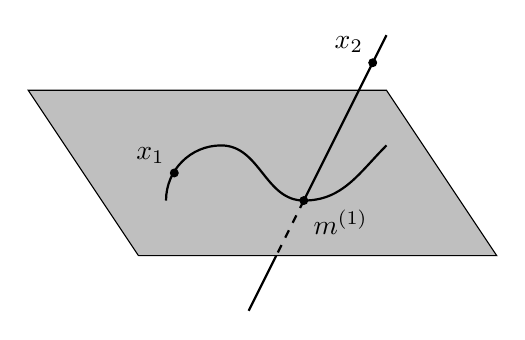
\begin{tikzpicture}[scale=0.7]
  \draw [fill=gray!50] (-.5,-1) -- (6,-1) -- (4,2) -- (-2.5,2) -- (-.5,-1);
  \draw [thick] (0,0) to [out=90,in=180] (1,1) to [out=0,in=180] (2.5,0) to [out=0,in=-135] (4,1);
  \draw [thick] (2.5,0) to (4,3);
  \draw [thick,dashed] (2.5,0) to (2,-1);
  \draw [thick] (2,-1) -- (1.5,-2);
  \draw [fill] (3.75,2.5) circle [radius=2pt] node[above left]{$x_2$};
  \draw [fill] (.15,.5) circle [radius=2pt] node[above left]{$x_1$};
  \draw [fill] (2.5,0.0) circle [radius=2pt] node[below right]{$m^{(1)}$};
 \end{tikzpicture}
\end{center}
and the invariants which contribute take the form
\begin{equation*} \bigg\langle \dfrac{\rho_i}{z-\psi_1},\rho^h\bigg\rangle_{0,2,\beta^{(0)}}^Y \bigg\langle \rho_h, \mathbbm 1_{X}\bigg\rangle_{0,(m^{(1)},0),\beta^{(1)}}^{X|Y} \end{equation*}
for $i = 1, \ldots, k$ and $h = 1, \ldots, l$. By computing dimensions, we find
\begin{align*}
0\leq \codim \rho^h &= \dim Y-\codim \rho_h \\
&= \dim Y-\vdim \Q{0}{(m^{(1)},0)}{X|Y}{\beta^{(1)}} \\
&= \dim Y-(\dim X-3-K_{X}\cdot \beta^{(1)}+2-m^{(1)})\\
&= K_Y \cdot \beta^{(1)} - Y \cdot \beta^{(1)}+m^{(1)} \\
&\leq 0
\end{align*}
where the final equality follows from adjunction and the final inequality holds because $-K_Y$ is nef and $m^{(1)}\leq Y \cdot \beta_1$. This shows that the only non-trivial contributions come from curve classes $\beta^{(1)}$ such that $K_Y \cdot \beta^{(1)}=0$, and that in this case the order of tangency must be maximal, i.e. $m^{(1)}=Y \cdot \beta^{(1)}$. Furthermore we must have $\codim \rho^h = 0$ and so $\rho^h = \rho^1 = \mathbbm{1}_Y$ which implies $\rho_h = \rho_1 = [\pt_Y]$. Finally since $m^{(1)}=Y \cdot \beta^{(1)}$ we have
\begin{equation*} m = Y \cdot \beta^{(0)}+m^{(1)}=Y \cdot (\beta^{(0)} + \beta^{(1)}) = Y \cdot \beta \end{equation*}
and so again this piece only contributes to $T_{0,(Y\cdot\beta)}^{X|Y}(z,\beta)$, and the contribution is:
\begin{equation*} \sum_{i=1}^k \left( \sum_{\substack{0 < \beta^{(1)} < \beta \\ K_Y \cdot \beta^{(1)}=0}} (Y \cdot \beta^{(1)}) \bigg\langle \dfrac{\rho_i}{z-\psi_1}, \mathbbm{1}_Y \bigg\rangle_{0,2,\beta-\beta^{(1)}}^Y \bigg\langle \rho_1, \mathbbm{1}_X \bigg\rangle_{0,(Y \cdot \beta^{(1)},0),\beta^{(1)}}^{X|Y} \right) \eta^i \end{equation*}
where the $Y \cdot \beta^{(1)}$ factor comes from the weighting on the virtual class of the comb locus. Finally, we must examine the terms of $T_{0,(m)}^{X|Y}(z,\beta)$ coming from:
\begin{equation*}\ev_{1*}(m\virt{\Q{0}{(m,0)}{X|Y}{\beta}})\end{equation*} 
Notice that we only have insertions from $i^*\HH^*(X) \subseteq \HH^*(Y)$, since $\ev_1$ is viewed as mapping to $X$. On the other hand
\begin{align*} \vdim \Q{0}{(m,0)}{X|Y}{\beta} & = \dim X-3 -K_X \cdot \beta +2-m & \\
& = \dim X - 1 -K_Y \cdot \beta + Y \cdot \beta - m \ \ & \text{by adjunction} \\
& \geq \dim X - 1 + Y\cdot\beta - m \ \ & \text{since $-K_Y$ is nef} \\
& \geq \dim X - 1 \ \ & \text{since $m \leq Y \cdot \beta$} \end{align*}
where in the second line we have applied the projection formula to $i$, and thus have implicitly used Assumption (2), discussed in \S \ref{Subsection setup}; namely that every curve class on $X$ comes from a class on $Y$.

Consequently the only insertions that can appear are those of dimension $0$ and $1$. However, the restriction of the $0$-dimensional class $\eta_0 = [\pt_X]$ to $Y$ vanishes, as do the restrictions of all $1$-dimensional classes except for $\eta_1$ (by the definition of the dual basis, since $\eta^1 = Y$). Thus the only insertion is $i^*\eta_1=\rho_1=[\pt_Y]$, and since $\eta^1$ has dimension $1$ all the inequalities above must actually be equalities. Thus we only have a contribution if $-K_Y \cdot \beta = 0$ and $m = Y \cdot \beta$. The contribution to $T_{0,(Y\cdot\beta)}^{X|Y}(z,\beta)$ in this case is:
\begin{equation*} (Y \cdot \beta) \langle \rho_1 , \mathbbm{1}_X \rangle_{0,(Y \cdot \beta,0),\beta}^{X|Y} \eta^1 \end{equation*}

Thus we have calculated $T_{0,(m)}^{X|Y}(z,\beta)$ for all $m$; substituting into equation \eqref{eqn:G} we obtain
\begin{align*} \prod_{j=0}^{Y \cdot \beta} (Y + jz) & S_0^X(z,\beta) = T_{0,(Y\cdot\beta)}^{X|Y}(z,\beta) \\
= \ & \sum_{i=1}^k \left\langle \dfrac{\rho_i}{z-\psi_1}, \mathbbm{1}_Y \right\rangle_{0,2,\beta}^Y \eta^i + \\
& \sum_{i=1}^k \left( \sum_{\substack{0 < \beta^{(1)} < \beta \\ K_Y \cdot \beta^{(1)}=0}} (Y \cdot \beta^{(1)}) \bigg\langle \dfrac{\rho_i}{z-\psi_1}, \mathbbm{1}_Y \bigg\rangle_{0,2,\beta-\beta^{(1)}}^Y \bigg\langle \rho_1, \mathbbm{1}_X \bigg\rangle_{0,(Y \cdot \beta^{(1)},0),\beta^{(1)}}^{X|Y} \right) \eta^i + \\
& (Y \cdot \beta) \langle \rho_1 , \mathbbm{1}_X \rangle_{0,(Y \cdot \beta,0),\beta}^{X|Y} \eta^1
\end{align*}
where the third term only appears if $K_Y \cdot \beta=0$. We can rewrite this as:
\begin{align*} \prod_{j=0}^{Y \cdot \beta} (Y + jz) & S_0^X(z,\beta) \\
& = \tilde{S}_0^Y(z,\beta) + \sum_{\substack{0 < \beta^{(1)} \leq \beta \\ K_Y \cdot \beta^{(1)}=0}} \left( (Y \cdot \beta^{(1)}) \bigg\langle \rho_1, \mathbbm{1}_X \bigg\rangle_{0,(Y \cdot \beta^{(1)},0),\beta^{(1)}}^{X|Y} \right) \tilde{S}_0^Y(z,\beta-\beta^{(1)})
\end{align*}
It is now clear from the expression above that equation \eqref{eqn:mirror} in the statement of Theorem \ref{Theorem Quantum Lefschetz} holds, with:
\begin{equation*} P_0^X(q) = 1 + \sum_{\substack{\beta>0 \\ K_Y\cdot\beta=0}} q^\beta (Y\cdot\beta) \langle \rho_1,\mathbbm 1_{X}\rangle_{0,(Y\cdot\beta,0),\beta}^{X|Y} \end{equation*}
To complete the proof it thus remains to show that:
\begin{equation*} P_0^X(q) = 1 + \sum_{\substack{\beta>0 \\ K_Y\cdot\beta=0}} q^\beta(Y\cdot\beta)!\langle\psi_1^{Y\cdot\beta-1} [\pt_X],\mathbbm 1_{X}\rangle_{0,2,\beta}^X \end{equation*}
The aim therefore is to express the relative invariants
\begin{equation*} \langle \rho_1 , \mathbbm{1}_X \rangle_{0,(Y\cdot\beta,0),\beta}^{X|Y} \end{equation*}
in terms of absolute invariants of $X$. Unsurprisingly, we once again do this by applying Theorem \ref{Theorem general recursion}. We have:
\begin{align*} \virt{\Q{0}{(Y \cdot \beta,0)}{X|Y}{\beta}} = \ & ((Y\cdot\beta-1)\psi_1+\ev_1^*Y) \virt{\Q{0}{(Y\cdot\beta-1,0)}{X|Y}{\beta}} \ - \\
& \virt{\mathcal{D}_{(Y\cdot\beta-1,0),1}^{\mathcal Q}(X|Y,\beta)} \end{align*}
We begin by examining the contributions from the comb loci. As before, we have only contributions coming from combs with $0$ teeth and combs with $1$ tooth. The former contributions take the form
\begin{equation*} \langle \rho_1 , \mathbbm{1}_Y \rangle_{0,2,\beta}^Y \end{equation*}
which vanish because $\vdim{\Q{0}{2}{Y}{\beta}} = \dim Y -1 -K_Y\cdot\beta = \dim Y -1$ whereas the insertion has codimension $\dim Y$. The latter contributions take the form
\begin{equation*} \langle \rho_1 ,\rho^h\rangle_{0,2,\beta^{(0)}}^Y \langle \rho_h,\mathbbm 1_{X}\rangle_{0,(Y\cdot(\beta-\beta^{(0)})-1,0),\beta-\beta^{(0)}}^{X|Y}\end{equation*}
and these must also vanish since:
\begin{align*} \codim \rho^h & = \dim Y - \codim \rho_h \\
& = \dim Y - \vdim \Q{0}{(Y\cdot(\beta-\beta^{(0)})-1,0)}{X|Y}{\beta-\beta^{(0)}} \\
& = \dim Y - (\dim X - 3 - K_X \cdot (\beta - \beta^{(0)}) + 2 - Y \cdot (\beta - \beta^{(0)}) + 1) \\
&= -1 + K_X \cdot (\beta-\beta^{(0)}) + Y \cdot (\beta-\beta^{(0)}) \\
& = -1 + K_Y\cdot(\beta-\beta^{(0)}) \\
& \leq -1
\end{align*}
Thus the comb loci do not contribute at all. Applying this recursively (the same argument as above shows that we never get comb loci contributions), we find that
\begin{align*}
(Y\cdot\beta)\langle \rho_1 ,\mathbbm 1_{X}\rangle_{0,(Y\cdot\beta,0),\beta}^{X|Y} & = (Y\cdot\beta) \langle \eta_1 \prod_{j=0}^{Y\cdot\beta-1}(Y+j\psi_1) , \mathbbm{1}_X \rangle_{0,2,\beta}^X \\
& = (Y\cdot\beta)!\langle[ \pt_X]\psi_1^{Y\cdot\beta-1},\mathbbm 1_X\rangle_{0,2,\beta}^X
\end{align*}
where the second equality holds because $Y\cdot\eta_1=\eta^1 \cdot \eta_1 = [\pt_X]$ and $Y^2\cdot\eta_1=0$. This completes the proof of Theorem \ref{Theorem Quantum Lefschetz}. \end{proof}

\begin{cor}
 If $Y$ is Fano then there is no correction term:
\begin{equation*} \sum_{\beta\geq 0} q^\beta\prod_{j=0}^{Y\cdot\beta}(Y+jz)S_0^X(z,\beta) = \tilde{S}_0^Y(z,q) \end{equation*}
\end{cor}

\begin{cor}
Let $Y = Y_5 \subseteq  X = \PP^4$ be the quintic three-fold. Then
\begin{equation*} \tilde{S}_0^{Y_5}(z,q)=\dfrac{I_{\text{sm}}^{Y_5}(z,q)}{P(q)} \end{equation*}
where
\begin{equation*} I_{\text{sm}}^{Y_5}(z,q)=5H+\sum_{d>0}\frac{\prod_{j=0}^{5d}(H+jz)}{\prod_{j=0}^{d}(H+jz)^5} \ q^d \end{equation*}
and:
\begin{equation*} P(q)=1+\sum_{d>0}\frac{(5d)!}{(d!)^5}q^d \end{equation*}
\end{cor}
\begin{proof} Apply Theorem \ref{Theorem Quantum Lefschetz} and use the fact that the quasimap invariants of $\PP^4$ coincide with the Gromov--Witten invariants, which are well-known from mirror symmetry. \end{proof}

\begin{remark}
Theorem \ref{Theorem Quantum Lefschetz} agrees with \cite[Theorem~1]{CZ-mirror} when $X$ is a projective space.
\end{remark}

\subsection{Comparison with the work of Ciocan-Fontanine and Kim} \label{Subsection CFK comparison}
Here we briefly explain how to compare our Theorem \ref{Theorem Quantum Lefschetz} to a formula obtained by Ciocan-Fontanine and Kim. We assume that the reader is familiar with the paper \cite{CF-K-wallcrossing}, in particular \S4 and \S5 thereof. There they introduce (in the more general context of $\epsilon$-stable quasimaps) the following generating functions for quasimap invariants of $Y$:
\begin{enumerate}
\item The \emph{$J^{\epsilon}$-function}
\begin{equation*} J^\epsilon({\bf t}, z)=\sum_{m\geq 0,\beta\geq 0} \dfrac{q^\beta}{m!} (\ev_\bullet)_*\left( \prod_{i=1}^m \ev_i^*({\bf t}) \cap\operatorname{Res}_{F_0} \virt{\QGe{0}{m}{Y}{\beta}} \right) \end{equation*}
for $\mathbf{t} \in \HH^*(X)$. Here $\QGe{0}{m}{Y}{\beta}$ is the moduli space of $\epsilon$-stable  quasimaps with a parametrised component, $F_0$ is a certain fixed locus of the natural $\Gm$-action on this space, and $\ev_\bullet$ is the evaluation at the point $\infty \in \PP^1$ on the parametrised component. $\operatorname{Res}_{F_0}$ is the residue of the virtual class, i.e. the virtual class of the fixed locus divided by the Euler class of the virtual normal bundle (see \cite{GraberPandharipande} for details on virtual localisation). The variable $z$ is the $\Gm$-equivariant parameter.
\item The \emph{$S^\epsilon$-operator}
\begin{equation*}
 S^\epsilon(\mathbf{t},z)(\gamma)=\sum_{m\ge 0,\beta\ge 0}\frac{q^\beta}{m!} 
(\ev_1)_*\left( \dfrac{\ev_2^*(\gamma) \cdot \prod_{j=3}^{2+m} \ev_j^*({\bf t})}{z-\psi_1} \cap\virt{\Qe{0}{2+m}{Y}{\beta}} \right)
\end{equation*}
where $\mathbf{t}, \gamma \in \HH^*(X)$ and $z$ is a formal variable.
\item The \emph{$P^\epsilon$-series}
\begin{equation*}
 P^\epsilon({\bf t}, z)=\sum_{h=1}^k \rho^h \sum_{m\geq 0,\beta\geq 0} \frac{q^\beta }{m!} \left( \ev_1^*(\rho_h \boxtimes p_\infty) \cap \virt{\QGe{0}{1+m}{Y}{\beta}} \right) \end{equation*}
where $\mathbf{t} \in \HH^*(X)$ and $z$ is the $\Gm$-equivariant parameter. Here we view $\ev_1$ as mapping to $Y \times \PP^1$, and $p_\infty\in \HH^*_{\Gm}(\PP^1)$ is the equivariant cohomology class defined by setting $p_{\infty}|_0 =0$ and $p_{\infty}|_{\infty}=-z$.
\end{enumerate}
Given these definitions, Ciocan-Fontanine and Kim use localisation with respect to the $\Gm$-action on the parametrised space to prove the following formula \cite[Theorem 5.4.1]{CF-K-wallcrossing}:
\[
 J^\epsilon(\mathbf{t},z)=S^\epsilon(\mathbf{t},z)(P^\epsilon(\mathbf{t},z))
\]
They observe that if we set ${\bf t}=0$ and restrict to semi-positive targets, then the only class that matches non-trivially with ${P^\epsilon}|_{\mathbf{t}=0}$ is $[\pt_Y]$. Hence the above formula takes the simple form
\begin{equation} \label{Ciocan-Fontanine Theorem t zero}
 \frac{J^\epsilon |_{{\bf t}=0}}{\langle [\pt_Y],  P^\epsilon|_{{\bf t}=0}\rangle}=S^\epsilon(\mathbbm{1}_Y)|_{\mathbf{t}=0} = \mathbbm 1_Y+\sum_{h=1}^k \rho^h \left(\sum_{\beta> 0}q^\beta\left\langle\frac{\rho_h}{z-\psi},\mathbbm 1_Y\right\rangle_{0,2,\beta}^{Y,\epsilon} \right)\end{equation}
see \cite[Corollary 5.5.1]{CF-K-wallcrossing}. In our setting, $\epsilon=0+$ and $Y$ embeds as a very ample hypersurface in a toric Fano variety $X$. Our Theorem \ref{Theorem Quantum Lefschetz} makes explicit a consequence of formula \eqref{Ciocan-Fontanine Theorem t zero}. More precisely:
\begin{lem} We have the following relations between our generating functions and the generating functions of Ciocan-Fontanine and Kim:
\begin{align}
\label{J epsilon equation} i_*J^{0+}|_{\mathbf{t}=0} & = \sum_{\beta \geq 0} q^\beta \prod_{j=0}^{Y \cdot \beta} (Y + jz) S_0^X(z,\beta) \\
\label{P epsilon equation} \langle [\pt_Y], P^{0+}|_{\mathbf{t}=0} \rangle & = P_0^X(q) \\
\label{S epsilon equation} i_*S^{0+}(\mathbbm{1}_Y)|_{\mathbf{t}=0} & = \tilde{S}^Y_0(z,q)
\end{align}
\end{lem}
\begin{proof}
\eqref{S epsilon equation} is clear from the second equality of \eqref{Ciocan-Fontanine Theorem t zero} and the definition of $\tilde{S}^Y_0(z,q)$. To show  \eqref{J epsilon equation}, let us look more closely at the left-hand side:
\begin{equation*} {J^{0+}}|_{{\mathbf{t}=0}} = \sum_{\beta\geq 0}q^\beta(\ev_\bullet)_* \left( \operatorname{Res}_{F_0}\virt{\QG{0}{0}{Y}{\beta}} \right) \end{equation*}
We have a diagram of fixed loci and evaluation maps
\bcd
\QG{0}{0}{Y}{\beta}\ar[d,hook,"i"]\ar[dr,phantom,"\Box"] & F_0^Y\ar[d, hook, "i"]\ar[l,hook']\ar[r,"\ev_{\bullet}"] & Y\ar[d,hook,"i"] \\
\QG{0}{0}{X}{\beta} & F_0^X\ar[l,hook']\ar[r,"\ev_{\bullet}"] & X
\ecd
and by a mild generalisation of \cite[Propositions 6.2.2 and 6.2.3]{CFKM}, we have an equality of $\Gm$-equivariant classes
\begin{equation*} i_*\virt{\QG{0}{0}{Y}{\beta}}=e(\pi_* E^Y_{0,0,\beta})\cap \virt{\QG{0}{0}{X}{\beta}} \end{equation*} 
where $\pi$ is the universal curve on $\QG{0}{0}{X}{\beta}$ and $E^Y_{0,0,\beta}$ is the equivariant line bundle\footnote{This is the parametrised analogue of the bundle $L_Y$ constructed in the definition of relative quasimaps; see \S \ref{Subsection relative stable quasimaps}.} on this curve associated to $\mathcal O_X(Y)$.
 
We would like to pull back this equation to the fixed locus $F_0^X$ in order to obtain an equation involving the residues. Let us first briefly recall the definition of $F_0^X$. Since there are no markings, any quasimap in $\QG{0}{0}{X}{\beta}$ has irreducible source curve. For such a quasimap to be $\Gm$-fixed we need that the induced rational map is constant; this means that the degree of the quasimap is concentrated at the basepoints (i.e. the sum of the lengths of the basepoints should be equal to the degree). Furthermore only the points $0$ and $\infty$ of the parametrised component are allowed to be basepoints. The fixed loci are thus indexed by ordered partitions of the degree which record the length of the basepoints at $0$ and $\infty$. $F_0^X$ is the locus on which all the degree is concentrated at $0$. This means that $\infty$ is not a basepoint and we have an evaluation map $\ev_\infty$ (denoted $\ev_{\bullet}$ earlier). See \cite[\S 4]{CF-K-wallcrossing} for more details: our $F_0^X$ is there denoted $F^{0,0,0}_{0,0,\beta}$.

Since the fibres of $\pi$ are irreducible and rational, the degree of the universal line bundle on the parametrised component is constant; therefore we have for $0 < j \leq Y\cdot\beta + 1$ an exact sequence:
\begin{equation*} 0 \to \pi_* (E^Y_{0,0,\beta}(-j\sigma_\infty)) \to \pi_* E^Y_{0,0,\beta} \to \sigma_\infty^*\mathcal{P}^{j-1}(E^Y_{0,0,\beta}) \to 0 \end{equation*}
where $\mathcal{P}^{j-1}$ denotes the bundle of $(j-1)$-jets, and $\sigma_{\infty}$ is the section given by the point $\infty \in \PP^1$ of the parametrised component. The right-hand map is given by evaluating a section of $E_{0,0,\beta}^Y$ (as well as its derivatives up to order $j-1$) at the point $\infty$. The left-hand term consists of sections of $E_{0,0,\beta}^Y$ which vanish at $\sigma_\infty$ to order $j$. If we set $j=Y\cdot\beta+1$ then this term vanishes and we have:
\begin{equation*} \pi_* E_{0,0,\beta}^Y = \sigma_\infty^* \mathcal{P}^{Y\cdot\beta}(E_{0,0,\beta}^Y) \end{equation*}
On the other hand, we have
\begin{equation*} 0 \to E^Y_{0,0,\beta} \otimes \omega_\pi^{\otimes j} \to \mathcal{P}^{j}(E^Y_{0,0,\beta}) \to \mathcal{P}^{j-1}(E^Y_{0,0,\beta}) \to 0
\end{equation*}
see \cite[\S 2]{Ga}. Pulling back along $\sigma_\infty$ and taking Euler classes, we can compute recursively from $j = Y \cdot \beta$ to $0$ and obtain a splitting
\begin{equation*}
e(\pi_* E^Y_{0,0,\beta})=\prod_{j=0}^{Y\cdot\beta} c_1(\sigma_\infty^* E^Y_{0,0,\beta}\otimes \omega_{\infty}^{\otimes j})
\end{equation*}
where $\omega_\infty=\sigma_\infty^*\omega_\pi$ gives the cotangent space at the point $\infty$. The bundle $\omega_\infty$ is (non-equivariantly) trivial since the source curves in $F_0^X$ are rigid; on the other hand the weight of the $\Gm$-action on the cotangent space at $\infty$ is $z$. We thus obtain:
\begin{equation*} i_*\virt{F_0^Y}=\prod_{j=0}^{Y\cdot\beta}(\ev_\infty^* Y+jz)\cap \virt{F_0^X} \end{equation*}
Furthermore, the Euler classes of the virtual normal bundles match under $i$. Substituting into $i_*J^{0+}|_{\mathbf{t}=0}$ we find that:
\begin{align*} i_* {J^{0+}}|_{{\mathbf{t}=0}} & = \sum_{\beta\geq 0}q^\beta(i\circ\ev_\bullet)_* \left( \operatorname{Res}_{F_0^Y}\virt{\QG{0}{0}{Y}{\beta}} \right) \\
& = \sum_{\beta \geq 0} q^\beta \prod_{j=0}^{Y \cdot \beta} (Y + jz) (\ev_{\bullet})_* \left( \operatorname{Res}_{F_0^X}\virt{\QG{0}{0}{X}{\beta}} \right) \end{align*}
On the other hand, if we apply \eqref{Ciocan-Fontanine Theorem t zero} with $X$ instead of $Y$, then the denominator on the left-hand side vanishes since $X$ is Fano. Comparing coefficients of $q^\beta$ we thus obtain
\begin{equation*} (\ev_{\bullet})_* \operatorname{Res}_{F_0^X}\virt{\QG{0}{0}{X}{\beta}} = S_0^X(z,\beta) \end{equation*}
from which it follows that:
\begin{equation*} i_*J^{0+}|_{\mathbf{t}=0} = \sum_{\beta \geq 0} q^\beta \prod_{j=0}^{Y\cdot\beta}(Y+jz) S_0^X(z,\beta)\end{equation*}
This proves \eqref{J epsilon equation}. It remains to show \eqref{P epsilon equation}. According to Ciocan-Fontanine and Kim, if we write the $1/z$-expansion of ${J^{\epsilon}}|_{\mathbf{t}=0}$ as
\begin{equation*} {J^{\epsilon}}|_{\mathbf{t}=0}=J^{\epsilon}_{0}(q)\mathbbm 1_Y+O(1/z) \end{equation*}
then $\langle [\pt_Y],  P^\epsilon|_{{\bf t}=0}\rangle=J^{\epsilon}_{0}(q)$. It thus remains to prove that $J^{0+}_0(q)=P_0^X(q)$.

Since $X$ is a toric Fano variety, we have the following calculation of residues due to Givental \cite{Givental-mirror} (see also \cite[Definition 7.2.8]{CF-K}):
\begin{align*}
S_0^X(z,\beta) =\prod_{\rho\in\Sigma_X(1)}\dfrac{\prod_{j=-\infty}^0(D_{\rho}+jz)}{\prod_{j=-\infty}^{D_{\rho}\cdot \beta}(D_\rho+jz)}
=\dfrac{\prod_{\substack{\rho \colon D_\rho \cdot \beta\leq 0}} \prod_{j=D_\rho \cdot \beta}^0 (D_{\rho}+jz)}{\prod_{\substack{\rho\colon D_\rho \cdot\beta > 0}} \prod_{j=1}^{D_\rho\cdot\beta} (D_{\rho}+jz)}
\end{align*}
We can then apply equation \eqref{J epsilon equation} to find $i_*J^{0+}|_{\mathbf{t}=0}$, and hence also to find $J^{0+}_0(q)$. In the end we obtain:
\begin{equation*}
 J^{0+}_0(q)=\sum_{\beta\geq 0}q^\beta(Y\cdot\beta)!\frac{\prod_{\rho\colon D_\rho\cdot\beta< 0}(-1)^{-D_{\rho}\cdot\beta}(-D_{\rho}\cdot\beta)!}{\prod_{\rho\colon D_\rho\cdot\beta> 0}(D_{\rho}\cdot\beta)!}
\end{equation*}
On the other hand the coefficient
\begin{equation*} \langle[\pt_X]\psi_1^{Y\cdot\beta-1},\mathbbm 1_X\rangle_{0,2,\beta}^X\end{equation*}
which appears in our $P_0^X(q)$-series also appears in $S_0^X(z,\beta)$. So again we can find it by appealing to Givental's calculation of $S_0^X(z,q)$.
\begin{align*}
 \langle[\pt_X]\psi_1^{Y\cdot\beta-1},\mathbbm 1_X\rangle_{0,2,\beta}^X &=\operatorname{coeff}_{q^\beta z^{-Y\cdot\beta}}\langle [\pt_X],S_0^X(z,q) \rangle\\
& =\frac{\prod_{\rho\colon D_\rho\cdot\beta< 0}(-1)^{-D_{\rho}\cdot\beta}(-D_{\rho}\cdot\beta)!}{\prod_{\rho\colon D_\rho\cdot\beta> 0}(D_{\rho}\cdot\beta)!}
\end{align*}
which proves \eqref{P epsilon equation}. We thus conclude that \eqref{Ciocan-Fontanine Theorem t zero} implies our Theorem~\ref{Theorem Quantum Lefschetz}. \end{proof}

\appendix

\section{The comparison morphism} \label{Section comparison morphism}
In this appendix we recall the construction of the comparison morphism for $\PP^N$ and how it can be used to show that the stable map and the quasimap invariants of projective space coincide. This has been proven in \cite[Theorem 3]{MOP} and \cite[Section 4.3]{Manolache-Push} (but see also \cite[Proposition 4.1]{Bertram} and \cite[Theorem 7.1]{Popa-Roth} for inspiration).

\subsection{Construction of the comparison morphism}
In order to give a morphism $\chi\colon\M{g}{n}{\PP^N}{d}\to\Q{g}{n}{\PP^N}{d}$ we need to be able to associate, to a family of stable maps on a base $B$, a family of quasimaps on the same base.

The pointwise construction is as follows: any stable map defines a quasimap with no basepoints. The only thing that might prevent this quasimap from being stable is the presence of rational tails (of positive degree, by the stability condition for stable maps). Let $C=C^{(0)}\sqcup_{q_i}R_i$ be the source curve; there is a ``permanent'' subcurve $C^{(0)}$ which is joined to a number of rational tails $R_i$ each of which has degree $d_i>0$. We let $q_i$ be the node connecting $C^{(0)}$ and $R_i$; note that it is the only special point of $R_i$, and hence all the marked points belong to $C^{(0)}$. We obtain a stable quasimap by collapsing the rational tails and introducing basepoints of length $d_i$ at each of the (former) nodes $q_i$.

In other words, the comparison map is given by sending the quasimap $((C,x_1,\ldots,x_n),L,u_0,\ldots,u_N))$ to 
\begin{equation*}((C^{(0)},x_1,\ldots,x_n),L|_{C^{(0)}}(\Sigma_i d_i q_i),\hat{u}_0,\ldots,\hat{u}_N) \end{equation*}
where $\hat{u}_i$ is obtained from $u_i|_{C^{(0)}}$ via the natural inclusion:
\begin{equation*} L|_{C^{(0)}}\to L|_{C^{(0)}}(\Sigma_i d_i q_i) \end{equation*}
Locally around $q_j$ this has the effect of multiplying each $u_i$ by the $d_j$th power of the equation defining $q_j$, thus introducing a basepoint of length $d_j$.

The construction in families requires us to find a line bundle on the universal curve that is trivial on the rational tails (which we wish to contract) and relatively ample elsewhere. This can be performed at the level of Picard stacks: let $\mathfrak{Pic}_{g,n}^{d,\text{st}}$ be the open substack of $\mathfrak{Pic}(\pi\colon\mathfrak{C}_{g,n}\to\mathfrak{M}_{g,n})$ obtained by requiring that the total degree of the line bundle is $d$, the degree on each component is nonnegative and $\mathcal L\otimes\omega_{\pi}(\Sigma_i x_i)$ is ample relative to $\pi$, where $\mathcal L$ is the universal line bundle.

Let $T^{\delta}$ be the locus in the universal curve $\mathfrak{C}_{\mathfrak{Pic}}$ over $\mathfrak{Pic}_{g,n}^{d,\text{st}}$ consisting of rational tails on which $\mathcal L$ has degree $\delta$; since the stack $\mathfrak{C}_{\mathfrak{Pic}}$ is smooth, $T^{\delta}$ is a Cartier divisor. Notice that $T^{\delta_0}$ and $T^{\delta_1}$ (say with $\delta_0<\delta_1$) intersect in a stratum of codimension $1$, where the rational tail splits into two rational components, the furthest from $C^{(0)}$ having degree $\delta_0$:

\begin{center}
\begin{tikzpicture}
 \draw[help lines] (-1,-1) grid (1,1);
 \node[below] at (0,-1) {$T^{\delta_0}$};
 \node[right] at (1,0) {$T^{\delta_1}$};
 
 \draw[gray] (0,-.5) -- (-2,0);
 \draw[decorate,decoration={snake,amplitude=2pt}] (-4,0) -- (-2.5,0);
 \draw (-3.8,-.2) -- node[left]{$\delta_0$} (-3.8,1.3);
 
 \draw[gray] (0,0) -- (-.5,1.5);
 \draw[-,decorate,decoration={snake,amplitude=2pt}] (-1,2) -- (.5,2);
 \draw (-.8,1.8) -- node[left]{$\delta_1-\delta_0$} (-.8,3.3);
 \draw (-1,3) -- node[above]{$\delta_0$} (0.5,3.5);
 
 \draw[gray] (.5,0) -- (2,.5);
 \draw[decorate,decoration={snake,amplitude=2pt}] (2.5,.5) -- (4,.5);
 \draw (2.7,.3) -- node[left]{$\delta_1$} (2.7,1.8);
 
\draw[fill=black] (0,0) circle [radius=1.5pt];
 \draw[fill=black] (0,-.5) circle [radius=1.5pt];
 \draw[fill=black] (.5,0) circle [radius=1.5pt];
 \end{tikzpicture}
\end{center}
\medskip

Define the following line bundle on $\mathfrak{C}_{\mathfrak{Pic}}$:
\begin{equation*} \mathcal N=\mathcal L\otimes\omega_{\pi}(\Sigma_i x_i)\otimes\bigotimes_{0<\delta\leq d}\mathcal O_{\mathfrak{C}_{\mathfrak{Pic}}}((\delta-1) T^\delta) \end{equation*}
We claim that $\mathcal{N}$ is trivial on every component of every rational tail, and $\pi$-relatively ample elsewhere. Consider a curve $C^{(0)}\sqcup_q R$ with a rational tail of degree $e$. We first consider the simple case where $R$ is isomorphic to a chain of $\PP^1$s. We label the components $R^{(1)},\ldots,R^{(n)}$, numbered from the closest to the farthest from $C^{(0)}$. We let $e_i$ denote the degree of $R^{(i)}$. We set $T_i=\bigcup_{j=i}^n R_j$ and $\epsilon_i=\deg \mathcal{L}|_{T_i} - 1 = e-1-\sum_{j=1}^{i-1} e_j$. The picture is as follows:

\begin{center}
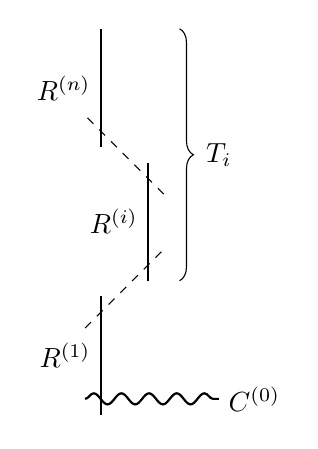
\begin{tikzpicture}
  \draw[thick,decorate,decoration={snake,amplitude=2pt}] (-.2,.2) -- (1.5,.2);
  \node[right] at (1.5,.2) {$C^{(0)}$};
  \draw[thick] (0,0) -- node[left]{$R^{(1)}$} (0,1.5);
  \draw[dashed] (-.2,1.1) -- (.8,2.1);
  \draw[thick] (.6,1.7) -- node[left]{$R^{(i)}$} (.6,3.2);
  \draw[dashed] (.8,2.8) -- (-.2,3.8);
  \draw[thick] (0,3.4) -- node[left]{$R^{(n)}$} (0,4.9);
  \draw [decorate,decoration={brace,amplitude=5pt,mirror}] (1,1.7) -- (1,4.9) node [midway,xshift=.5cm]{$T_i$};
 \end{tikzpicture}
\end{center}

The local structure of $\mathfrak{Pic}_{g,n}^{d,\text{st}}$ means that a general one-parameter family inside this stack will give us a smoothing of our curve. The total space of such a family is a normal surface $S$; thus we can compute the degree of the restriction of $\mathcal{N}$ to the irreducible components of the central fiber of this family by first restricting $\mathcal{N}$ to $S$, and then using intersection theory on the normal surface $S$.

Notice first that $T^\delta|_S = T_{i_\delta}$ where $i_\delta$ is the unique value of $i$ such that
\begin{equation*} \delta = \sum_{j=i_{\delta}}^n e_i \end{equation*}
and if no such $i_\delta$ exists then $T^\delta|_S = 0$. Thus we obtain:
\begin{equation*} \bigotimes_{0<\delta\leq d}\mathcal{O}_{\mathfrak{C}_{\mathfrak{Pic}}}((\delta-1) T^\delta)|_S = \mathcal{O}_S(\Sigma_{j=1}^n \epsilon_j T_j) \end{equation*}
Now, $R^{(i)}$ has self-intersection $-2$ for $i=1,\ldots,n-1$, and so we have
\begin{equation*}
R^{(i)}\cdot T_j =
  \begin{cases}
    0 & \text{for } j<i \\
    -1 & \text{for } j=i \\
    1 & \text{for } j=i+1 \\
    0 & \text{for } j>i+1
  \end{cases}
\end{equation*}
from which it follows that:
\begin{equation*} \deg \mathcal{N}|_{R^{(i)}} = \deg \mathcal{L}|_{R^{(i)}} - \epsilon_i + \epsilon_{i+1} = e_i - e_i = 0 \end{equation*}
On the other hand $R^{(n)}$ has self-intersection $-1$ and so we have
\begin{equation*}
R^{(n)} \cdot T_j =
\begin{cases}
0 & \text{for } j < n \\
-1 & \text{for } j = n
\end{cases}
\end{equation*}
which implies:
\begin{equation*} \deg \mathcal{N}|_{R^{(n)}} = \deg \mathcal{L}|_{R^{(n)}} - 1 - \epsilon_n = e_n - 1 - (e_n-1) = 0\end{equation*}
Here we have used the fact that $\omega_\pi(\Sigma_i x_i)$ has degree $0$ on $R^{(i)}$ for $i=1,\ldots,n-1$ and has degree $-1$ on $R^{(n)}$. Thus $\mathcal{N}$ is trivial on every component on every rational tail, as claimed. The fact that it is $\pi$-relatively ample on the rest of the curve follows from the stability condition and the fact that $\OO_{\mathfrak{C}_{\mathfrak{Pic}}}(T^\delta)$ is effective when restricted to $C^{(0)}$.

In the above discussion we restricted ourselves to the simple case where $R$ is a chain of $\PP^1$s. In general, however, $R$ can be an arbitrary tree of $\PP^1$s. The argument in this case is similar, though combinatorially more complex. For brevity we will discuss one example:

\begin{center}
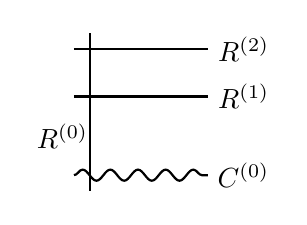
\begin{tikzpicture}
  \draw[thick,decorate,decoration={snake,amplitude=2pt}] (-.2,.2) -- (1.5,.2);
  \node[right] at (1.5,.2) {$C^{(0)}$};
  \draw[thick] (0,0) -- (0,2);
  \node[left] at (0.1,.7) {$R^{(0)}$};
  \draw[thick] (-.2,1.2) -- (1.5,1.2) node[right]{$R^{(1)}$};
  \draw[thick] (-.2,1.8) -- (1.5,1.8) node[right]{$R^{(2)}$};
\end{tikzpicture}
\end{center}

Here $R$ has $3$ irreducible components $R^{(0)},R^{(1)},R^{(2)}$ with degrees $e_0,e_1,e_2$ respectively. Let $e = e_0+e_1+e_2$ be the total degree of the rational tail.

Of the divisors $T^{\delta}$ for $0<\delta\leq d$, the total space $S$ only intersects\footnote{Notice in particular that $S$ does not intersect $T^{e_0}$ or $T^{e_0+e_1}$ (unless $e_0=0$).} $T^{e_1}, T^{e_2}$ and $T^e$. We have:
\begin{align*}
T^{e_1}|_S & = R^{(1)} \\
T^{e_2}|_S & = R^{(2)} \\
T^e|_S & = R = R^{(0)} + R^{(1)} + R^{(2)}
\end{align*}
Let us first look at $R^{(1)}$. This has self-intersection $-1$ and so:
\begin{equation*} R^{(1)} \cdot T^{e_1}|_S = -1 \qquad R^{(1)} \cdot T^{e_2}|_S = 0 \qquad R^{(1)} \cdot T^e|_S = 1-1 = 0 \end{equation*}
Thus we obtain
\begin{equation*} \deg \mathcal{N}|_{R^{(1)}} = \deg \mathcal{L}|_{R^{(1)}} - 1 - (e_1 - 1) = 0 \end{equation*}
and same argument applies to $R^{(2)}$. On the other hand, $R^{(0)}$ has self-intersection $-3$ (in general, a component that appears with $n$ adjacent components will have self-intersection $-n$). We have
\begin{equation*} R^{(0)} \cdot T^{e_1}|_S = 1 \qquad R^{(0)} \cdot T^{e_2}|_S = 1 \qquad R^{(0)} \cdot T^e|_S = -3 + 1 + 1 = -1 \end{equation*}
and thus we obtain
\begin{align*} \deg \mathcal{N}|_{R^{(0)}} & = \deg \mathcal{L}|_{R^{(0)}} + 1 + (e_1 - 1) + (e_2 - 1) - (e-1) \\
& = e_0 + e_1 + e_2 - e = 0 \end{align*}
as required.

To summarise, then: we have constructed a line bundle $\mathcal{N}$ on $\mathfrak{C}_{\mathfrak{Pic}}$ which is trivial on the components that we wish to contract and $\pi$-relatively ample elsewhere. By taking the relative Proj construction we therefore obtain another curve
\begin{equation*} \hat{\mathfrak{C}}_{\mathfrak{Pic}}:=\underline{\operatorname{Proj}}_{\mathfrak{Pic}_{g,n}^{d,\operatorname{st}}} \left(\bigoplus_{k\geq 0}\pi_*\mathcal{N}^{\otimes k}\right) \end{equation*}
over $\mathfrak{Pic}_{g,n}^{d,\text{st}}$, and a map $\sst$ which contracts the rational tails
\bcd
\mathfrak C_{\mathfrak{Pic}}\ar[r,"\sst"]\ar[dr,"\pi" left=3pt] & \hat{\mathfrak{C}}_{\mathfrak{Pic}} \ar[d,"\hat{\pi}"]\\
 & \mathfrak{Pic}_{g,n}^{d,\text{st}}
\ecd
The map $\hat{\pi}$ is flat since it is a family of genus $g$ curves over a reduced base. Furthermore, it can be checked using cohomology and base-change \cite[Theorem 12.11]{HAR} \cite[Corollary 1.5]{Knudsen} (notice that the fibers of $\sst$ are either points or rational curves) that
\begin{equation*}\hat{\mathcal L}:=\sst_*\left(\mathcal L\otimes \bigotimes_{0<\delta\leq d}\mathcal{O}_{\hat{\mathfrak{C}}_{\mathfrak{Pic}}}(\delta T^\delta)\right) \end{equation*}
is a line bundle on $\hat{\mathfrak{C}}_{\mathfrak{Pic}}$ of degree $d$ relative to $\hat{\pi}$. By the Yoneda lemma we thus obtain a comparison morphism $\tilde{\comp}$ fitting into a commutative diagram:
\bcd
\mathfrak C_{\mathfrak{Pic}}\ar[r,"\sst"]\ar[dr,"\pi" left=3pt] & \hat{\mathfrak{C}}_{\mathfrak{Pic}} \ar[d,"\hat{\pi}"]\ar[dr,phantom,"\square" right=-0.5pt]\ar[r] & \mathfrak C_{\mathfrak{Pic}}\ar[d,"\pi"] \\
 & \mathfrak{Pic}_{g,n}^{d,\text{st}}\ar[r,"\tilde{\comp}"] & \mathfrak{Pic}_{g,n}^{d,\text{st}}
\ecd
This discussion all took place at the level of Picard stacks. If we work instead at the level of stable maps and quasimaps the same arguments apply to construct the contracted curve $\hat{\mathcal{C}}_{\mathcal{M}}$ and line bundle $\hat{\mathcal{L}}$. Furthermore we can push down the sections $u_i$ from $\mathcal{C}_{\mathcal{M}}$ to $\hat{\mathcal{C}}_{\mathcal{M}}$ because they are constant on the contracted rational tails (notice that they automatically acquire basepoints). This gives rise to a comparison morphism:
\begin{equation*} \comp\colon \M{g}{n}{\PP^N}{d}\to\Q{g}{n}{\PP^N}{d} \end{equation*}
We have a commutative diagram
\bcd
\M{g}{n}{\PP^N}{d} \ar[d,"\nu_{\mathcal{N}}"]\ar[r,"\comp"] & \Q{g}{n}{\PP^N}{d}\ar[d,"\nu_{\mathcal Q}"] \\
\mathfrak{Pic}_{g,n}^{d,\text{st}}\ar[r,"\tilde{\comp}"] & \mathfrak{Pic}_{g,n}^{d,\text{st}}
\ecd
and, as before, a diagram of universal curves:
\bcd
\mathcal C_{\mathcal{M}}\ar[r,"\sst"] \ar[rd,"\pi_{\mathcal{N}}" left=3pt] & \hat{\mathcal{C}}_{\mathcal{M}}=\comp^*\mathcal C_{\mathcal Q} \ar[d,"\hat{\pi}_{\mathcal{N}}"]\ar[dr,phantom,"\square"]\ar[r] & \mathcal C_{\mathcal Q}\ar[d,"\pi_{\mathcal Q}"] \\
 & \M{g}{n}{\PP^N}{d}\ar[r,"\comp"] & \Q{g}{n}{\PP^N}{d}
\ecd

\subsection{The comparison morphism preserves the virtual classes}
For $\PP^N$ the stable map and quasimap invariants coincide; we have:
\begin{equation*} \comp_* \virt{\M{g}{n}{\PP^N}{d}} = \virt{\Q{g}{n}{\PP^N}{d}} \end{equation*}
The proof of this fact, following \cite{Manolache-Push}, rests on the construction of a relative perfect obstruction theory
\begin{equation*} \mathbf{E}_{\comp} \to \mathbf{L}_{\comp} \end{equation*}
for the morphism $\comp$. The construction is best outlined in the arXiv version of \cite[Remark 5.20]{Manolache-Push}. Let $\tilde{\nu}_{\mathcal{N}}$ denote the composition:
\bcd
\M{g}{n}{\PP^N}{d} \ar[r,"\nu_{\mathcal{N}}"] \ar[rr,"{\tilde{\nu}}_{\mathcal{N}}", bend right=25pt] & \mathfrak{Pic}_{g,n}^{d,\operatorname{st}} \ar[r,"\tilde{\comp}"] & \mathfrak{Pic}_{g,n}^{d,\operatorname{st}}
\ecd
We may endow this morphism with a relative perfect obstruction theory via the following morphism of exact triangles:
\bcd
\nu_\mathcal{N}^*\mathbf L_{\tilde{\comp}}\ar[d]\ar[r] & \mathbf E_{\tilde{\nu}_{\mathcal{N}}} \ar[d]\ar[r] & \mathbf E_{\nu_\mathcal{N}} \ar[d]\ar[r,"{[1]}"] & {}\\
\nu_\mathcal{N}^*\mathbf L_{\tilde{\comp}}\ar[r] & \mathbf L_{\tilde{\nu}_{\mathcal{N}}} \ar[r] & \mathbf L_{\nu_\mathcal{N}} \ar[r,"{[1]}"] & {}
\ecd
Notice that $\tilde{\comp}$ is a morphism between smooth Artin stacks. As such we can examine the exact triangle of cotangent complexes induced by $\tilde{\comp}$ and conclude that $\mathbf{L}_{\tilde{\comp}}$ is supported in $[-1,1]$. It then follows easily  that $\mathbf E_{\tilde{\nu}_{\mathcal{N}}}$ is also supported in $[-1,1]$; in order to show that it is perfect, we consider the long exact cohomology sequence near $\h^1(\mathbf E_{\tilde{\nu}_{\mathcal{N}}})$:
\begin{equation*} \h^{0}(\mathbf E_{\nu_\mathcal{N}}) \to \h^{1}(\nu_\mathcal{N}^*\mathbf L_{\tilde{\comp}}) \to \h^{1} (\mathbf E_{\tilde{\nu}_{\mathcal{N}}}) \to 0 \end{equation*}
We must show that the morphism $\h^0 (\mathbf{E}_{\nu_{\mathcal{N}}}) \to \h^1(\nu_{\mathcal{N}}^* \mathbf{L}_{\tilde{\comp}})$ is surjective. Looking at the dual picture, we see that the map
\begin{equation*} \h^{1}(\nu_\mathcal{N}^*\mathbf{L}_{\tilde{\comp}})^\vee \to \h^{0}(\mathbf E_{\nu_\mathcal{N}})^\vee \cong \h^{0}(\mathbf{L}_{\nu_\mathcal{N}})^\vee \end{equation*}
is injective, because every infinitesimal automorphism of the rational tail induces a nontrivial deformation of the stable map, since the degree of the stable map is positive on every component of the rational tail. We conclude that $\h^{1}\mathbf E_{\tilde{\nu}_{\mathcal{N}}}=0$ and so indeed $\mathbf{E}_{\tilde{\nu}_{\mathcal{N}}}$ is a perfect obstruction theory for $\tilde{\nu}_{\mathcal{N}}$. It induces the usual virtual fundamental class on the moduli space of stable maps.

Now, we can construct a morphism of obstruction theories (see 
\cite[Lemma 4.19]{Manolache-Push})
\begin{equation*} \comp^*\mathbf E_{\nu_\mathcal Q}\to\mathbf E_{\nu_\mathcal{N}} \end{equation*}
as follows. We have
\begin{align*} \mathbf E^\vee_{\nu_\mathcal{N}}& =\R\pi_{\mathcal{N}*}\mathcal L^{\oplus N+1}=\R\hat\pi_* \sst_*\mathcal L^{\oplus N+1} \\
\comp^*\mathbf E^\vee_{\nu_\mathcal Q} & = \chi^* \R \pi_{\mathcal{Q}} \hat{\mathcal{L}}^{\oplus{N+1}} = \R {\hat{\pi}}_{\mathcal{N}*}\hat{\mathcal L}^{\oplus N+1}\end{align*}
where $\hat{\mathcal L}=\sst_*\left(\mathcal L\otimes \bigotimes_{0<\delta\leq d}\mathcal O_{\mathfrak C}(\delta T^\delta)\right)$. Thus $\mathbf E^\vee_{\nu_\mathcal{N}}\to\comp^*\mathbf E^\vee_{\nu_\mathcal Q}$ comes from the following inclusion of line bundles on $\mathcal C_\mathcal{N}$:
\[
\mathcal L\hookrightarrow \mathcal L\otimes \bigotimes_{0<\delta\leq d}\mathcal O_{\mathfrak C}(\delta T^\delta).
\]
We now claim that this morphism factors through $\mathbf E_{\tilde{\nu}_{\mathcal{N}}}$. Examining the diagram:
\bcd
& \comp^*\mathbf E_{\nu_\mathcal Q}\ar[dl,dashed,"\exists ?"]\ar[d]\ar[dr,"\phi"] & \\
\mathbf E_{\tilde{\nu}_{\mathcal{N}}} \ar[r] & \mathbf E_{\nu_\mathcal{N}}\ar[r] & \nu_\mathcal{N}^*\mathbf L_{\tilde{\comp}}[1] \ar[r,"{[1]}"] & \,
\ecd
we see that it is equivalent to show that $\phi$ is the zero map. This follows formally from the factorisation:
\bcd
 & & \mathbf L_\comp \ar[ld,"{[1]}" swap] & & \\
\comp^* \mathbf E_{\nu_\mathcal Q}\ar[dd]\ar[r] & \comp^*\mathbf L_{\nu_\mathcal Q}\ar[rr] &  & \mathbf L_{\tilde{\nu}_{\mathcal{N}}}\ar[ul]\ar[dd] & \\
 & & & & \nu_{\mathcal{N}}^*\mathbf L_{\tilde{\comp}}[1]\ar[ul,"{[1]}" swap] \\
\mathbf E_{\nu_\mathcal{N}} \ar[rrr] & & & \mathbf L_{\nu_\mathcal{N}}\ar[ur] & {}
\ecd
We thus obtain a morphism
\begin{equation*} \psi \colon \comp^* \mathbf{E}_{\nu_{\mathcal{Q}}} \to \mathbf{E}_{\tilde{\nu}_{\mathcal{N}}} \end{equation*}
and the cone $C(\psi)$ gives a relative obstruction theory for the comparison morphism $\chi$. A priori, it is supported in $[-2,0]$. By the octahedral axiom we have:
%-------------
\begin{comment}
\begin{center}
\begin{tikzcd}[execute at end picture={
    \begin{scope}[on background layer]
    \fill[pattern=north east lines, pattern color=gray!20] (a.north west) -- (b.north east) -- (b.south east) -- (a.south west) -- cycle;
    \fill[pattern=north west lines, pattern color=gray!20] (c.north west) -- (c.north east) -- (d.south east) -- (d.south west) -- cycle;
    \end{scope}
  }]
\comp^* \mathbb E_{\nu_\mathcal Q}\ar[d]\ar[r] & |[alias=a]| \comp^*\mathbb L_{\nu_\mathcal Q}\ar[r] & |[alias=c]|\mathbb L_{\tilde{\nu}_{\mathcal{N}}}\ar[r]\ar[d] & |[alias=b]| \mathbb L_\comp \\
\mathbb E_{\nu_\mathcal{N}} \ar[rr] & & \mathbb L_{\nu_\mathcal{N}}\ar[d] & \\
 & & |[alias=d]| \nu_{\mathcal{N}}^*\mathbb L_{\comp '}[1]
\end{tikzcd}
\end{center} 
\end{comment}
\begin{comment}
Dually, we look at $\nu_\mathcal{N}^*\mathbb T_{\tilde{\comp}}[-1]\xrightarrow{\phi^\vee} \R\hat\pi_*(\hat{\mathcal L}^{\oplus r+1})$. Notation: call $R$ the rational tail, joined at the rest of the curve (which we denote by $(C^{(0)},\mathbf p)$ as a marked curve), at the node $q$, which we may occasionally think of as a (smooth) point on $C^{(0)}$. We claim that:
\begin{itemize}
 \item $h^0(\phi^\vee)$ is zero because: the LHS involves automorphisms of the rational tail that leave $C^{(0)}$ fixed, while the RHS involves deformations of $C^{(0)}$, so there is no possible interference.
 \item $h^1(\phi^\vee)$ is zero because: \textcolor{red}{this is slightly awkward.} There are two types of possible contributions to the LHS. They correspond to either moving the node $q$ along $C^{(0)}$, or smoothing it. The former appears in the relative tangent of $\chi'$ only if the marked curve $(C^{(0)},\mathbf p)$ has no automorphisms that may ``move $q$ back'', i.e. $(C^{(0)},\mathbf p)$ is a stable pointed curve. The latter matters only if $(C^{(0)},q,\mathbf p)$ has no moduli, i.e. $(C^{(0)},\mathbf p)$ is a rational tail with less than 3 markings. \textcolor{red}{I will try to justify why the first type vanishes under $h^1(\phi^\vee)$, and leave the second type because I do not understand it as yet.} Look at the long exact sequence
\begin{align*}
  0 &\to \Hom(\Omega_{C^{(0)}},\mathcal O_{C^{(0)}}(-q-\sum p_i)) &\to \Hom(\Omega_{C^{(0)}},\mathcal O_{C^{(0)}}(-\sum p_i)) &\to \\
  T_{C^{(0)},q} &\to \Ext^1(\Omega_{C^{(0)}},\mathcal O_{C^{(0)}}(-q-\sum p_i)) &\to \Ext^1(\Omega_{C^{(0)}},\mathcal O_{C^{(0)}}(-\sum p_i)) &\to 0
 \end{align*}
We are interested in what happens to
\[
 \frac{T_{C^{(0)},q}}{\operatorname{Im}\left( \Hom(\Omega_{C^{(0)}},\mathcal O_{C^{(0)}}(-\sum p_i)) \right)}
\]
under $h^1(\phi^\vee)$. If we can show that $h^1(\phi^\vee)$ factors through $\Ext^1(\Omega_{C^{(0)}},\mathcal O_{C^{(0)}}(-\sum p_i))$ we are in business. Indeed the natural maps
\bcd
\Def_L\ar[d]\ar[r] & \Def_{(C,L)}\ar[d]\ar[r] & \Def_C\ar[d] \\
H^1(\mathcal O_C)\ar[r] & H^1(L^{\oplus r+1})\ar[r] & H^1(f^*T_{\PP^N})
\ecd
show that $h^1(\phi^\vee)$ factors through
\[
\Ext^1(\Omega_{C^{(0)}},\mathcal O_{C^{(0)}}(-q-\sum p_i))\to \Ext^1(\Omega_{C^{(0)}},\mathcal O_{C^{(0)}})\to \Ext^1(f^*\Omega_{\PP^N},\mathcal O_{C^{(0)}})\simeq H^1(f^*T_{\PP^N}).
\]
 \item $h^2(\phi^\vee)$ is zero because: $\mathbb E^\vee_{\tilde{\nu}_{\mathcal{N}}}$ is supported in $[0,1]$.
\end{itemize}
\end{comment}
%----------------------
\begin{center}
 \begin{tikzcd}[cramped]
  \comp^*\mathbf E_{\nu_\mathcal{Q}} \ar[dd,"\psi"]\ar[rrdd,"\tilde{\psi}"] & & & & & & \\
& & & & & & \\
\mathbf E_{\tilde{\nu}_\mathcal{N}}\ar[dd]\ar[rr] & & \mathbf E_{\nu_\mathcal{N}} \ar[rrrr]\ar[dr] & & & & \nu_{\mathcal{N}}^*\mathbf L_{\tilde{\comp}}{[1]} \\
& & & C(\tilde{\psi})\ar[urrr] & & & \\
C(\psi) \ar[urrr] & & & & & & 
 \end{tikzcd}
\end{center}
Now $C(\psi)$ is supported in $[-1,0]$ \cite[Lemma 4.20]{Manolache-Push} and $\nu_{\mathcal{N}}^*\mathbf L_{\tilde{\comp}}{[1]}$ is supported in degrees $[-2,0]$, from which it follows that $C(\psi)=\mathbf E_{\comp}$ is a perfect obstruction theory. The conclusion, that
\begin{equation*} \comp_*\virt{\M{g}{n}{\PP^N}{d}}=\virt{\Q{g}{n}{\PP^N}{d}} \end{equation*}
follows from the connectedness of $\M{g}{n}{\PP^N}{d}$ \cite{KP}, hence of $\Q{g}{n}{\PP^N}{d}$, and an application of the virtual push-forward theorem \cite[Proposition 4.21]{Manolache-Push}.

\subsection{An example where the comparison morphism fails to exist}
We will now explain with an example the reason why a naive attempt to extend the comparison morphism to a general toric variety fails. The problem boils down to the fact that not all toric divisors are nef: a rational tail contained in a such divisor may have a corresponding line bundle with negative degree $-d$; when contracting such a rational tail, we take the line bundle $L|_{C^{(0)}}(-dq)$, but it is not clear what to do with the sections. We would like to divide them by $z^d$, where $z$ is a local coordinate around $q$, but we are by no means guaranteed that this is possible. Put differently, we now have an inclusion $L|_{C^{(0)}}(-dq)\hookrightarrow L|_{C^{(0)}}$, but the given sections of $L$ do not necessarily live in the image of $H^0(C^{(0)},L|_{C^{(0)}}(-dq))\to H^0(C^{(0)},L|_{C^{(0)}})$.

A concrete example can be found by looking at the Hirzebruch surface $\mathbb F_1=\operatorname{Bl}_{p}\PP^2$. Since we may choose the point $p$ to be a torus-fixed point of $\PP^2$, $\mathbb{F}_1$ is a toric variety; see Figures \ref{Figure toric fan}, \ref{Figure nef cone} and \ref{Figure Mori cone}.
\begin{figure}[h]
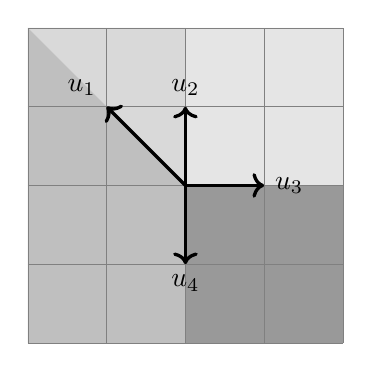
\begin{tikzpicture}
\path [fill=black!10!white] (0,0) -- (2,0) -- (2,2) -- (0,2) -- (0,0);
\path [fill=black!15!white] (0,0) -- (-2,2) -- (0,2) -- (0,0);
\path [fill=black!25!white] (0,0) -- (-2,2) -- (-2,-2) -- (0,-2) -- (0,0);
\path [fill=black!40!white] (0,0) -- (0,-2) -- (2,-2) -- (2,0) -- (0,0);
\draw [help lines] (-2,-2) grid (2,2);
\draw [->,very thick] (0,0) -- (-1,1) node[above left]{$u_1$};
\draw [->,very thick] (0,0) -- (0,1) node[above]{$u_2$};
\draw [->,very thick] (0,0) -- (1,0) node[right]{$u_3$};
\draw [->,very thick] (0,0) -- (0,-1) node[below]{$u_4$};
\end{tikzpicture}
\caption{Toric fan for $\mathbb F_1$.}
\label{Figure toric fan}
\end{figure}
\begin{figure}
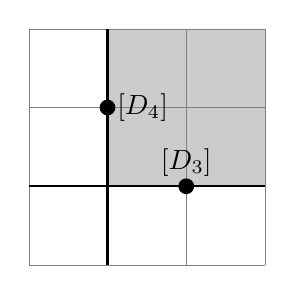
\begin{tikzpicture}
\path [fill=black!20!white] (0,0) -- (2,0) -- (2,2) -- (0,2) -- (0,0);
\draw [help lines] (-1,-1) grid (2,2);
\fill [black] (0,1) circle[radius=.1] node[right]{${[D_4]}$};
\fill [black] (1,0) circle[radius=.1] node[above]{${[D_3]}$};
\draw [thick] (-1,0) -- (2,0);
\draw [thick] (0,-1) -- (0,2);
\end{tikzpicture}
\caption{Nef cone $\operatorname{Nef}(\mathbb F_1)$.}
\label{Figure nef cone}
\end{figure}
\begin{figure}
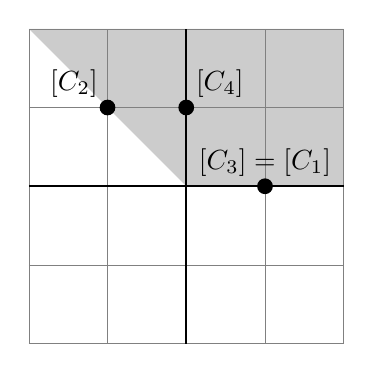
\begin{tikzpicture}
\path [fill=black!20!white] (0,0) -- (2,0) -- (2,2) -- (-2,2) -- (0,0);
\draw [help lines] (-2,-2) grid (2,2);
\fill [black] (0,1) circle[radius=.1] node[above right]{${[C_4]}$};
\fill [black] (1,0) circle[radius=.1] node[above]{${[C_3]}={[C_1]}$};
\fill [black] (-1,1) circle[radius=.1] node[above left]{${[C_2]}$};
\draw [thick] (-2,0) -- (2,0);
\draw [thick] (0,-2) -- (0,2);
\end{tikzpicture}
\caption{Mori cone $\overline{\operatorname{NE}}(\mathbb F_1)$.}
\label{Figure Mori cone}
\end{figure}

The group $\Pic(\mathbb F_1)$ is generated by $[D_3]$ and $[D_4]$, with relations $[D_1]=[D_3]$ and $[D_2]=[D_4]-[D_3]$; the intersection form is given by:
\[
{}
\begin{cases}
 [D_3]^2=0 \\
 [D_3]\cdot [D_4]=1 \\
 [D_4]^2=1
\end{cases} 
\]
When we are thinking of the $D_i$ as curves instead of as divisors, we will denote them by $C_i$. The space $\mathbb F_1$ can be viewed as a $\PP^1$-bundle over $\PP^1$, in which case $C_1$ and $C_3$ represent the fibers of the bundle (over the torus-fixed points of $\PP^1$), while $C_4$ and $C_2$ are the zero and infinity sections, respectively. When thinking of $\mathbb F_1$ as $\operatorname{Bl}_{p}\PP^2$, $C_2$ is the exceptional divisor, $C_4$ is the toric line not passing through $p$, and $C_1,C_3$ are the strict transforms of the toric lines through $p$.

Let us examine the moduli space $\M{0}{2}{\mathbb F_1}{[C_2]+[C_4]}$. Since $[C_4] = [C_2]+[C_3]$ we have $[C_2]+[C_4] = 2[C_2] + [C_3]$. We can thus consider the locus of stable maps inside this moduli space such that:
\begin{enumerate}
\item the source curve splits up as $C=R_1 \sqcup_q R_2$, with all of the marked points belonging to $R_1$;
\item $R_1$ is mapped isomorphically to a fibre (hence $f_*[R_1] = [C_3]$);
\item $R_2$ is a degree-$2$ covering of $C_2 \cong \PP^1$ (hence $f_*[R_2]=2[C_2]$).
\end{enumerate}
The component $R_2$ is a rational tail and so should be contracted by the comparison morphism. However, the line bundle $L_2$ on $C$ corresponding to the divisor $D_2$ has degree $-2$ when restricted to $R_2$ (the degree is equal to $[D_2] \cdot f_*[R_2]=2[D_2]^2 = -2$). Thus when we contract $R_2$ we should replace $L_2|_{R_1}$ by $L_2|_{R_1}(-2q)$. However, the section $u_2|_{R_1}$ only comes from a section of $L_2|_{R_1}(-2q)$ if it vanishes to order $2$ at $q$, that is, $q$ is a ramification point for the degree $2$ cover. This is certainly not the case in general. Thus we see that in this example the comparison morphism does not exist.

\begin{comment}

\textcolor{blue}{Something is going on here: in this case there is a boundary component where the map is of the type that we have just described, and the requirement that $u_{2|R_1}$ vanishes of order $2$ at the node defines precisely the intersection with the main component. Check this. Could we possibly exploit this phenomenon to define a smaller compactification, possibly even smaller than quasimaps?} 

\end{comment}

\section{Notes on quasimaps}\label{Section quasimap theory}
In this appendix we collect several foundational results in quasimap theory, including:
\begin{enumerate}
\item \ilemph{Functoriality} (\S \ref{Functoriality of Quasimap Spaces Section}): given a morphism $f\colon Y\to X$ we describe the induced map:
\begin{equation*} \om{Q}(f)\colon\Q{g}{n}{Y}{\beta}\to\Q{g}{n}{X}{f_*\beta} \end{equation*}
We also discuss (\S \ref{section:rel_pot_for_qm_functoriality}) when $\om{Q}(f)$ admits a compatible perfect obstruction theory.
\item \ilemph{Splitting axiom} (\S \ref{Subsection splitting}): this gives an equality between two natural virtual classes on boundary strata (i.e. loci where the underlying curve is reducible of a prescribed type).
\item \ilemph{Comparison with the GIT construction} (\S \ref{Section comparison with GIT construction}): we show that for a (not necessarily toric) hypersurface $Y \hookrightarrow X$, our definition of $\om{Q}(Y)$ as a substack of $\om{Q}(X)$ coincides with the definition of $\om{Q}(Y)$ given by the description of $Y$ as a GIT quotient (see \cite{CFKM}).
\end{enumerate}

\subsection{Functoriality} \label{Functoriality of Quasimap Spaces Section}

In the case of stable maps, a morphism $f : Y \to X$ induces a morphism between the corresponding moduli spaces
\begin{equation*}\om{M}(f) : \M{g}{n}{Y}{\beta} \rightarrow \M{g}{n}{X}{f_* \beta} \end{equation*}
given by post-composition with $f$ and (if necessary) stabilisation of the source curve. Because of this, we may say that the construction of the moduli space of stable maps is \ilemph{functorial}.

It is natural to ask whether the same holds for the moduli space of quasimaps, i.e. whether we have a morphism:
\begin{equation*} \om{Q}(f) : \Q{g}{n}{Y}{\beta} \to \Q{g}{n}{X}{f_* \beta} \end{equation*}
Since here the objects of the moduli space are not maps, we cannot simply compose with $f$. Nevertheless, our definition should be equivalent to composing with $f$ when applied to a quasimap without any basepoints. In \cite[Section 3.1]{CF-K-wallcrossing} a definition (in the GIT context) is given when $f$ is an embedding into a projective space; we shall discuss the general situation of a morphism between toric varieties $f\colon Y\to X$.

Our approach uses the language of $\Sigma$--collections introduced by D. A. Cox. This approach is natural insofar as a quasimap is a generalisation of a $\Sigma$--collection. We will refer extensively to \cite{CoxRing} and \cite{CoxFunctor}.

Let $X$ and $Y$ be smooth and proper toric varieties with fans $\Sigma_X \subseteq N_X$ and $\Sigma_Y \subseteq N_Y$. Suppose we are given $f : Y \to X$, which we do not assume to be a toric morphism. By \cite[Theorem 1.1]{CoxFunctor} the data of such a map is equivalent to a $\Sigma_X$--collection on $Y$:
\begin{equation*} ( (L_\rho, u_\rho)_{\rho \in \Sigma_X(1)}, (\varphi_{m_x})_{m_x \in M_X} ) \end{equation*}
In addition, \cite{CoxRing} allows us to describe line bundles on $Y$ and their global sections in terms of the homogeneous coordinates $(z_\tau)_{\tau \in \Sigma_Y(1)}$. All of these observations are combined into the following theorem, which is so useful that we will state it here in its entirety:

\begin{thm} \cite[Theorem 3.2]{CoxFunctor} \label{CoxTheorem} The data of a morphism $f:Y \to X$ is the same as the data of homogeneous polynomials
\begin{equation*} P_\rho \in S^Y_{\beta_\rho} \end{equation*}
for $\rho = f^* \OO_X(D_\rho) \in \Sigma_X(1)$, where $\beta_\rho \in \Pic Y$ and $S^Y_{\beta_\rho}$ is the corresponding graded piece of the Cox ring:
\begin{equation*}S^Y = \CC[z_\tau : \tau \in \Sigma_Y(1)]\end{equation*}
These data are required to satisfy the following two conditions:
\begin{enumerate}
\item $\sum_{\rho \in \Sigma_X(1)} \beta_\rho \otimes n_\rho = 0$ in $\Pic Y \otimes N_X$, where $n_\rho$ is the principal generator of the ray $\rho$.
\item $(P_\rho(z_\tau)) \notin Z(\Sigma_X) \subseteq \Aaff^{\Sigma_X(1)}$ whenever $(z_\tau) \notin Z(\Sigma_Y) \subseteq \Aaff^{\Sigma_Y(1)}$.
\end{enumerate}
Furthermore, two such sets of data $(P_\rho)$ and $(P^\prime_\rho)$ correspond to the same morphism if and only if there exists a $\lambda \in \Hom_\Z(\Pic X, \Gm)$ such that
\begin{equation*} \lambda(D_\rho) \cdot P_\rho = P^\prime_\rho \end{equation*}
for all $\rho \in \Sigma_X(1)$. Finally, if we define $\tilde{f}(z_\tau) = (P_\rho(z_\tau))$ then this defines a lift of $f$ to the prequotients:
\bcd
\Aaff^{\Sigma_Y(1)} \setminus Z(\Sigma_Y) \ar[r, "\tilde{f}"] \ar[d, "q_Y"] & \Aaff^{\Sigma_X(1)} \setminus Z(\Sigma_X) \ar[d,"q_X"] \\
Y \ar[r, "f"] & X
\ecd
\end{thm}
\begin{aside} Throughout this section we will stick to the notation established above; in particular we will use $\rho$ to denote a ray in $\Sigma_X(1)$ and $\tau$ to denote a ray in $\Sigma_Y(1)$. \end{aside}

Recall our goal: given a map $f \colon Y \to X$ we wish to define a ``push-forward'' map:
\begin{equation*} \om{Q}(f) : \Q{g}{n}{Y}{\beta} \to \Q{g}{n}{X}{f_*\beta} \end{equation*}
Consider therefore a quasimap
\begin{equation*} ((C,x_1,\ldots,x_n), (L_\tau, u_\tau)_{\tau \in \Sigma_Y(1)}, (\varphi_{m_Y})_{m_Y \in M_Y}) \in \Q{g}{n}{Y}{\beta} \end{equation*}
over an arbitrary base. Pick data $(P_\rho)_{\rho \in \Sigma_X(1)}$ corresponding to the map $f$, as in the theorem above; we will later see that our construction does not depend on this choice.

The idea of the construction is as follows. Locally around a point $x~\in~U_x \subseteq C$ we can trivialise the $L_\tau$ to obtain a morphism to the prequotient
\begin{equation*} (u_\tau)_\tau \colon U_x \to \Aaff^{\Sigma_Y(1)} \end{equation*}
which lifts the induced rational map to $Y$. On the other hand the data of $(P_\rho)_\rho$ gives a lifting of $f\colon Y\to X$ to a morphism between the prequotients
\begin{equation*}(P_\rho)_\rho \colon \Aaff^{\Sigma_Y(1)} \to \Aaff^{\Sigma_X(1)}\end{equation*}
and so the composed map to the prequotient of $X$ is given by:
\begin{equation*} (P_\rho((u_\tau)_\tau))_\rho : U_x \to \Aaff^{\Sigma_X(1)} \end{equation*}
In order to define the pushed-forward quasimap, we thus need to make sense of $P_\rho((u_\tau)_\tau)$ as a section of a certain line bundle $\tilde{L}_\rho$ on the curve.

We now make this precise. The first issue to address is the stabilisation of the source curve. The procedure is the same as in the case of stable maps: if $C_0 \subseteq C$ is a rational component with $2$ special points (hence with curve class $\beta_0 > 0$) and such that $f_* \beta_0 = 0$, then $C_0$ should be contracted when we pass to $X$. The possibilities are:

\begin{center}
\begin{tikzpicture}[scale=0.5]
\draw (0,0) -- (1,3) node[above]{$\beta_1$} (0,1) -- (1,-2) node[below]{$\beta_0$};
\draw[fill=black] (0.66,-1) circle[radius=2pt];
\draw[->,decorate,decoration=snake] (2,0.5) -- (4,0.5);
\draw (5,0) -- (6,3) node[above]{$f_*\beta_1$};
\draw[fill=black] (5.16,.5) circle[radius=2pt];

\draw (10.33,-1.5) -- node[right]{$\beta_0$} (10.33,2.5) (10,1) -- (11,4) node[above]{$\beta_1$} (10,0) -- (11,-3) node[below]{$\beta_2$};
\draw[->,decorate,decoration=snake] (12,0.5) -- (14,0.5);
\draw (15,0) -- (16,3) node[above]{$f_*\beta_1$} (15,1) -- (16,-2) node[below]{$f_*\beta_2$};
\end{tikzpicture}
\end{center}
To perform the contraction we need to construct a line bundle on $C$ that is trivial on the components which we wish to contract and ample (relative to the base) on all the other components.

Fix a polarisation $\OO_X(1)$ on $X$ and express $f^*\OO_X(1)$ in terms of the toric divisors of $Y$:
\begin{equation*} f^*\OO_X(1) = \bigotimes_\tau \OO_Y(D_\tau)^{\otimes c_\tau} \end{equation*}
Then the line bundle
\begin{equation*} \omega_{\pi}(x_1+\ldots+x_n)\otimes \bigotimes_\tau L_\tau^{\otimes a_\tau} \end{equation*}
gives the required contraction by taking relative Proj. We thus obtain a curve $\tilde{C}$ and a morphism $\phi : C \to \tilde{C}$ which contracts the unstable components.

Recall that for $\rho \in \Sigma_X(1)$, $P_\rho$ is a polynomial in the $z_\tau$. We can thus write it as
\begin{equation} \label{Prho} P_\rho(z_\tau) = \sum_{\underline{a}} P_\rho^{\underline{a}}(z_\tau) = \sum_{\underline{a}} \mu_{\underline{a}} \prod_{\tau} z_{\tau}^{a_{\tau}} \end{equation}
where the sum is over a finite number of multindices $\underline{a} = (a_\tau) \in \N^{\Sigma_Y(1)}$ and the $\mu_{\underline{a}}$ are nonzero scalars. Observe that, for each $\underline{a}$, the line bundle $\otimes_\tau  L_\tau^{\otimes a_\tau}$ on $C$ is trivial on the components contracted by $\phi$ (which are always rational). Hence, by cohomology and base-change, it descends to a line bundle on $\tilde{C}$:
\begin{equation*} \tilde{L}_\rho^{\underline{a}} :=\phi_* \bigotimes_\tau L_\tau^{\otimes a_\tau} \end{equation*}
We may then take the following section of $\tilde{L}_\rho^{\underline{a}}$:
\begin{equation*} \tilde{u}_\rho^{\underline{a}} = P_\rho^{\underline{a}}(u_\tau) := \mu_{\underline{a}} \prod_\tau u_\tau^{a_\tau}; \end{equation*}
A priori this is really a section of $\otimes_\tau L_\tau^{\otimes a_\tau}$ on $C$; but since it is constant on the components contracted by $\phi$, it descends to a section of $\tilde{L}_\rho^{\underline{a}}$ on $\tilde{C}$.

Thus, each of the terms $P_\rho^{\underline{a}}$ of $P_\rho$ defines a section $\tilde{u}_\rho^{\underline{a}}$ of a line bundle $\tilde{L}_\rho^{\underline{a}}$ on $\tilde{C}$. What we want, however is a single section $\tilde{u}_\rho$ of a single line bundle $\tilde{L}_\rho$. This is where the isomorphisms $\varphi_{m_Y}$ come in.

Recall that we have a short exact sequence:
\begin{equation} \label{Pic short exact sequence for Y} 0 \longrightarrow M_Y \overset{\theta}{\longrightarrow} \Z^{\Sigma_Y(1)} \longrightarrow \Pic Y \longrightarrow 0 \end{equation}
Let $\underline{a}$ and $\underline{b}$ be multindices appearing in the sum \eqref{Prho} above. By the homogeneity of $P_\rho$ we have
\begin{equation*} \sum_\tau a_\tau [D_\tau] = \beta_\rho = \sum_\tau b_\tau [D_\tau] \end{equation*}
which is precisely the statement that in the above sequence $\underline{a}$ and $\underline{b}$ map to the same element of $\Pic Y$ (namely $\beta_\rho$). Hence there exists a unique $m_Y \in M_Y$ such that:
\begin{equation*} \theta(m_Y) = \underline{a} - \underline{b} \end{equation*}
Now, the isomorphism $\varphi_{m_Y}$ (contained in the data of our original quasimap) is a map:
\begin{equation*} \varphi_{m_Y} : \bigotimes_\tau L_\tau^{\otimes \langle m_Y, n_\tau \rangle} \cong \OO_{C} \end{equation*}
By definition, $\theta(m_Y) = (\langle m_Y,n_\tau \rangle)_{\tau \in \Sigma_Y(1)}$. But also $\theta(m_Y) = (a_\tau - b_\tau)_{\tau \in \Sigma_Y(1)}$. Hence we have:
\begin{equation*} \varphi_{m_Y} : \bigotimes_\tau L_\tau^{\otimes a_\tau} \cong \bigotimes_\tau L_\tau^{\otimes b_\tau} \end{equation*}
This descends to give canonical isomorphisms
\begin{equation*} \tilde{L}_\rho^{\underline{a}} \cong \tilde{L}_\rho^{\underline{b}} \end{equation*}
for all $\underline{a}$ and $\underline{b}$. Let us choose one such $\underline{a}$ (it doesn't matter which); call it $\underline{a}^\rho$. We define:
\begin{equation*} \tilde{L}_\rho := \tilde{L}_\rho^{\underline{a}^\rho} \end{equation*}
Then for all $\underline{b}$ we can use the above isomorphisms to view $\tilde{u}_\rho^{\underline{b}}$ as a section of $\tilde{L}_\rho$. Summing all of these together we thus obtain a section $\tilde{u}_\rho$ of $\tilde{L}_\rho$, which we can write (with abuse of notation) as:
\begin{equation*} \tilde{u}_\rho = \sum_{\underline{a}} \mu_{\underline{a}} \prod_\tau u_\tau^{a_\tau} \end{equation*}
Note that if we had made a different choice of $\underline{a}^\rho$ above the result would have been isomorphic.

Thus far we have constructed line bundles and sections $(\tilde{L}_\rho, \tilde{u}_\rho)_{\rho \in \Sigma_X(1)}$ on $\overline{\mathcal C}$. It remains to define the isomorphisms
\begin{equation*} \tilde{\varphi}_{m_X} : \otimes_\rho \tilde{L}_\rho^{\otimes \langle m_X, n_\rho \rangle} \cong \OO_{\tilde{C}} \end{equation*}
for all $m_X \in M_X$. The left hand side is:
\begin{align*} \otimes_\rho \tilde{L}_\rho^{\otimes \langle m_X, n_\rho \rangle} & = \otimes_\rho \left( \phi_* \otimes_\tau L_\tau^{\otimes a_\tau^\rho} \right)^{\otimes \langle m_X, n_\rho \rangle} = \phi_* \otimes_\tau L_\tau^{\otimes \left( \sum_{\rho} a_\tau^\rho  \langle m_X, n_\rho \rangle \right)} \end{align*}
Now, for $m_Y \in M_Y$ we have isomorphisms $\varphi_{m_Y} : \otimes_\tau L_\tau^{\otimes \langle m_Y, n_\tau \rangle} \cong \OO_{C}$. In order to construct $\tilde{\varphi}_{m_X}$ it is therefore tempting to look for an $m_Y$ such that
\begin{equation*} \langle m_Y, n_\tau \rangle = \sum_\rho a_\tau^\rho \langle m_X, n_\rho \rangle \end{equation*}
for all $\tau \in \Sigma_Y(1)$ (we will then set $\tilde{\varphi}_{m_X} = \varphi_{m_Y}$). Consider therefore the short exact sequence \eqref{Pic short exact sequence for Y}. Recall that $\theta(m_Y) = (\langle m_Y, n_\tau \rangle)_{\tau \in \Sigma_Y(1)}$. Hence we need to show that
\begin{equation*} \left( \sum_\rho a_\tau^\rho \langle m_X, n_\rho \rangle \right)_{\tau \in \Sigma_Y(1)} \end{equation*}
belongs to the image of $\theta$, i.e. that it belongs to the kernel of the second map (notice that $m_Y$ is then unique because $\theta$ is injective). This is equivalent to saying that
\begin{equation*} \sum_\tau \sum_\rho a_\tau^\rho \langle m_X, n_\rho \rangle [D_\tau] = 0 \in \Pic Y \end{equation*}
Now, we have
\begin{equation*} \sum_\tau a_\tau^\rho [D_\tau] = \beta_\rho \end{equation*}
so that the above sum becomes
\begin{equation*} \sum_\rho \langle m_X, n_\rho \rangle \beta_\rho = \left\langle m_X, \sum_\rho \beta_\rho \otimes n_\rho \right \rangle = \langle m_X, 0 \rangle = 0 \end{equation*}
where $\sum_\rho \beta_\rho \otimes n_\rho = 0$ by Condition (1) in Theorem \ref{CoxTheorem}. So there does indeed exist a (unique) $m_Y \in M_Y$ such that $\langle m_Y, n_\tau \rangle = \sum_\rho a_\tau^\rho \langle m_X, n_\rho \rangle$, and we can set:
\begin{equation*} \tilde{\varphi}_{m_X} = \varphi_{m_Y} : \bigotimes_\rho \tilde{L}_\rho^{\otimes \langle m_X, n_\rho \rangle} \cong \OO_{\overline{\mathcal C}} \end{equation*}
Thus we have produced a quasimap with target $X$ and class $f_*\beta$ on the base $\Q{g}{n}{Y}{\beta}$:
\begin{equation*} ((\tilde{C},\tilde{x_1},\ldots,\tilde{x_n}), (\tilde{L}_\rho, \tilde{u}_\rho)_{\rho \in \Sigma_X(1)}, (\tilde{\varphi}_{m_X})_{m_X \in M_X}) \end{equation*}
The proof that this construction does not depend on the choice of $(P_\rho)$ is straightforward and is left to the reader.

It remains to demonstrate that the quasimap thus constructed is nondegenerate and stable. Nondegeneracy follows immediately from Condition (2) in Theorem \ref{CoxTheorem}. Put differently: the original quasimap defined a rational map $C \dashrightarrow Y$, whereas the new quasimap defines a rational map which is simply the composition $C \dashrightarrow Y \to X$ (up to contracting unstable components). Therefore the set of basepoints is exactly the same.

Stability follows precisely from the construction of $\phi$: if we write the polarisation of $X$ as $\OO_X(1) = \bigotimes_\rho \OO(D_\rho)^{\otimes b_\rho}$ then 
\begin{equation*} \omega_{\tilde{\pi}}(\bar x_1+\ldots \bar x_n)\otimes\bigotimes_\rho \tilde{L}_\rho^{\otimes b_\rho} \end{equation*}
will be $\tilde\pi$-ample on $\tilde{C}$, since we have contracted all the components on which $f^*\OO_X(1)$ was trivial without introducing any rational tail.

To summarise, we have explained how to canonically associate, to any family of quasimaps with target $Y$, a family of quasimaps with target $X$. This completes the proof of the following:

\begin{thm} \label{functoriality proposition} Let $X$ and $Y$ be smooth proper toric varieties and $f : Y \to X$ a morphism. Then there exists a natural push-forward map:
\begin{equation*} \om{Q}(f) \colon \Q{g}{n}{Y}{\beta} \to \Q{g}{n}{X}{f_* \beta} \end{equation*}\end{thm}
 	
\begin{remark}
 Theorem \ref{CoxTheorem} tells us that we can lift any morphism between toric varieties to an equivariant morphism between the prequotients
\bcd
 \Aaff^{\Sigma_Y(1)} \setminus Z(\Sigma_Y) \ar[r, "\tilde{f}"] \ar[d, "q_Y"] & \Aaff^{\Sigma_X(1)} \setminus Z(\Sigma_X) \ar[d,"q_X"] \\
 Y \ar[r, "f"] & X
\ecd
where the torus homomorphism
\begin{equation*} G_Y=\Hom_{\mathbb Z}(\Pic(Y), \Gm)\to G_X=\Hom_{\mathbb Z}(\Pic(Y),\Gm) \end{equation*}
is induced in the obvious way by $f\colon Y\to X$. Now, thinking of quasimaps as maps to the quotient stack, functoriality is again clear by postcomposition with $\tilde{f}$ (notice that the preimage of the unstable locus of $X$ is the unstable locus of $Y$).
\end{remark}

Finally, let us describe how this push-forward morphism behaves when $f$ is a nonconstant map $\PP^r \to \PP^N$. Write $f$ in homogeneous coordinates as:
\begin{equation*} f[z_0, \ldots, z_r] = [f_0(z_0, \ldots, z_r), \ldots, f_N(z_0, \ldots, z_r)] \end{equation*}
where the $f_i$ are all homogeneous of degree $a>0$. Then given a quasimap with target $\PP^r$
\begin{equation*} (C, L, u_o, \ldots, u_r) \end{equation*}
the pushed-forward quasimap with target $\PP^N$ is:
\begin{equation*} (C, L^{\otimes a}, f_0(u_0, \ldots, u_r) , \ldots, f_N(u_0, \ldots, u_r)) \end{equation*}

\subsection{Relative obstruction theories for $\om{Q}(Y)\to\om{Q}(X)$}\label{section:rel_pot_for_qm_functoriality}
Assume now that $f\colon Y\to X$ is a morphism (between projective varieties) satisfying any of the following three equivalent conditions:
\begin{enumerate}
 \item $f$ is finite;
 \item for any ample line bundle $\OO_X(1)$ on $X$, $f^*\OO_X(1)$ is ample on $Y$;
 \item for every effective curve class $\beta\in \HH_2^+(Y)$, $f_*\beta\neq 0$.
\end{enumerate}
These conditions are in particular satisfied when $f$ is a closed embedding, which is the case of most interest to us.

Observe then that the induced morphism $$k=\om{Q}(f) \colon \Q{g}{n}{Y}{\beta} \to \Q{g}{n}{X}{f_* \beta}$$ commutes with the projections to $\mathfrak M_{g,n}$, i.e. there is no need to stabilise the underlying curve. We would like to have a pull-back morphism $k^!$ between Chow groups. However, even in the easiest possible case when $f \colon Y \hookrightarrow X$ is a regular embedding, $k$ itself is not necessarily a regular embedding, and so the Gysin map in the sense of \cite{FUL} is not guaranteed to exist.

However, when $\Q{g}{n}{X}{f_* \beta}$ is unobstructed (for instance when $X=\PP^N$ and $g=0$ or $(g,n)=(1,0)$) there is a way around this. In \cite{Manolache-Pull} a generalisation of the Gysin map called the \ilemph{virtual pull-back} is defined for morphisms endowed with a relative perfect obstruction theory. Moreover, a sufficient condition is given \cite[Corollary 4.9]{Manolache-Pull} for this map to respect the virtual classes.

\begin{lem} \label{Exists relative POT} For a \emph{finite} morphism of smooth toric varieties $f\colon Y\to X$, there exists a relative obstruction theory $\EE_k$ for the morphism
\begin{equation*} k : \Q{g}{n}{Y}{\beta} \to \Q{g}{n}{X}{f_*\beta} \end{equation*}
which fits into a compatible triple with the standard obstruction theories for the quasimap spaces over $\MM_{g,n}$. Furthermore, $\EE_k$ is perfect \emph{if $\Q{g}{n}{X}{f_*\beta}$ is unobstructed}, so that:
\begin{equation*} k^!_{\operatorname{v}} [ \Q{g}{n}{X}{f_*\beta} ] = \virt{\Q{g}{n}{Y}{\beta}} \end{equation*} \end{lem}

\begin{proof} Note first that, since $k$ does not change the source curve of a quasimap, we indeed have a commuting triangle:
\bcd
\Q{g}{n}{Y}{\beta} \ar[rr,"k"] \ar[rd] & & \Q{g}{n}{X}{f_*\beta} \ar[ld] \\
& \MM_{g,n} & 
\ecd
We have perfect obstruction theories $\EE_{\om{Q}(Y)/\MM}$ and $\EE_{\om{Q}(X)/\MM}$ and we want to find a perfect obstruction theory $\EE_k$. Consider the diagram of universal curves
\bcd
\mathcal{C}_Y \ar[r,"\alpha"] \ar[d,"\pi"] \ar[rd,phantom,"\square" right] & \mathcal{C}_{X} \ar[d,"\rho"] \\
\Q{g}{n}{Y}{\beta} \ar[r,"k"] & \Q{g}{n}{X}{f_*\beta}
\ecd
which is cartesian because $k$ does not alter the source curve of any quasimap. We have sheaves $\mathcal{F}_Y$ and $\mathcal{F}_{X}$ on $\mathcal{C}_Y$ and $\mathcal{C}_{X}$ respectively such that:
\begin{align*} \EE_{\om{Q}(Y)/\MM}^\vee & = \R \pi_* \mathcal{F}_Y \\
\EE_{\om{Q}(X)/\MM}^\vee & = \R \rho_* \mathcal{F}_{X} \end{align*}
It follows (by flatness of $\rho$) that when we pull back the latter obstruction theory to $\om{Q}(Y)$ we obtain:
\begin{equation*} k^* \EE_{\om{Q}(X)/\MM}^\vee = \R \pi_* \alpha^* \mathcal{F}_{X} \end{equation*}
To construct a compatible triple, we require a morphism $k^* \EE_{\om{Q}(X)/\MM} \to \EE_{\om{Q}(Y)/\MM}$. Dually, it is therefore enough to construct a morphism of sheaves on $\mathcal{C}_Y$
\begin{equation*} \mathcal{F}_Y \to \alpha^* \mathcal{F}_{X} \end{equation*}
and then apply $\R \pi_*$. This is analogous to the morphism $f^* T_Y \to f^* T_{X}|_Y$ which is used in the stable maps setting. However the construction for quasimaps requires a little more ingenuity, because we do not have access to a universal map $f$.

The sheaf $\mathcal{F}_Y$ is defined on $\mathcal{C}_Y$ by the short exact sequence
\begin{equation*} 0 \to \OO_{\mathcal{C}_Y}^{\oplus r_Y} \to \oplus_{\tau} \mathcal{L}_\tau \to \mathcal{F}_Y \to 0 \end{equation*}
where $r_Y = \operatorname{rk} \Pic Y$ (implicitly we have chosen a basis for $\Pic Y$). Similarly $\mathcal{F}_{X}$ is defined on $\mathcal{C}_{X}$ by:
\begin{equation*} 0 \to \OO_{\mathcal{C}_{X}}^{\oplus r_X} \to \oplus_{\rho} \mathcal{L}_\rho \to \mathcal{F}_{X} \to 0 \end{equation*}
We will construct the map $\mathcal{F}_Y \to \alpha^* \mathcal{F}_{X}$ by first constructing a morphism:
\begin{equation*} \oplus_{\tau} \mathcal{L}_\tau \to \alpha^* (\oplus_{\rho} \mathcal{L}_\rho) \end{equation*}
Recall that $f\colon Y\to X$ is given by homogeneous polynomials
\begin{equation*} P_\rho \in S^Y_{\beta_\rho} \subset S^Y = k[z_\tau : \tau \in \Sigma_Y(1)] \end{equation*}
in the Cox ring of $Y$, where $\beta_{\rho}=f^*[D_\rho] \in \Pic Y$. For all monomials appearing in $P_\rho$, if we look at their exponents $(a_{\tau})_{\tau\in\Sigma_Y(1)}$, we have $\sum_{\tau\in\Sigma_Y(1)}a_\tau[D_\tau]=\beta_\rho$ by homogeneity; hence we can use the isomorphisms parametrised by $M_Y$ as in the proof of Proposition \ref{functoriality proposition} above in order to interpret the $(P_\rho)$ as a morphism
\begin{equation*} (P_\rho)_{\rho\in\Sigma_X(1)}\colon \bigoplus_{\tau} \mathcal{L}_{\tau} \to \bigoplus_{\rho} \bigotimes_{\tau} \mathcal{L}_\tau^{\otimes a_\tau^\rho} = \bigoplus_{\rho} \tilde{\mathcal{L}}_\rho = \alpha^* \left( \bigoplus_{\rho} \mathcal{L}_\rho \right) 
\end{equation*}
where the notation is as in the proof of functoriality in \S \ref{Functoriality of Quasimap Spaces Section}. Thus we have constructed a morphism $\oplus_{\tau} \mathcal{L}_\tau \to \alpha^* (\oplus_{\rho} \mathcal{L}_\rho)$.

On the other hand, $f\colon Y\to X$ induces a pullback map on line bundles $\Pic(X)\to\Pic(Y)$. Since we have implicitly chosen bases for these $\Z$-modules, this gives rise to a matrix, whose transpose we denote by:
\begin{equation*} Q\in \operatorname{Mat}_{r_X\times r_Y}(\Z) \end{equation*}
It is now clear by the functoriality construction that the left-hand square in the following diagram is commutative; hence it induces the (dashed) map of sheaves that we were after:
\begin{equation}\label{diagram:functoriality}
\begin{tikzcd}
0 \ar[r] & \OO_{C_Y}^{\oplus r_Y} \ar[r] \ar[d,"Q"] & \oplus_{\tau} \mathcal{L}_\tau \ar[r] \ar[d,"{(P_\rho)}"] & \mathcal{F}_Y \ar[d,dashed]\ar[r] & 0 \\
0 \ar[r] & \OO_{\mathcal{C}_{Y}}^{\oplus r_X} \ar[r] & \alpha^* \left(\oplus_{\rho} \mathcal{L}_\rho\right) \ar[r] & \alpha^* \mathcal{F}_{X} \ar[r] & 0
\end{tikzcd}
\end{equation}
Applying $\R \pi_*$ and dualising we obtain a morphism between the obstruction theories for the quasimap spaces, and we can complete this to obtain an exact triangle
\begin{equation*} k^* \EE_{\om{Q}(X)/\MM} \to \EE_{\om{Q}(Y)/\MM} \to \EE_k \xrightarrow{[1]}\end{equation*}
on $\om{Q}(Y)$. The axioms of a triangulated category then give a morphism of exact triangles:
\bcd
k^* \EE_{\om{Q}(X)/\MM} \ar[r] \ar[d] & \EE_{\om{Q}(Y)/\MM} \ar[r] \ar[d] & \EE_k  \ar[r,"{[1]}"] \ar[d] & \, \\
k^*\LL_{\om{Q}(X)/\MM} \ar[r] & \LL_{\om{Q}(Y)/\MM} \ar[r] & \LL_k \ar[r,"{[1]}"] & \,
\ecd
It follows from a simple diagram chase that $\EE_k \to \LL_k$ is a relative obstruction theory supported in $[-2,0]$. On the other hand, assuming that $\Q{g}{n}{X}{f_*\beta}$ is unobstructed, we may look at the long exact sequence in cohomology and find:
\begin{equation*} 0 \to \h^{-2}(\EE_k) \to \h^{-1}(k^* \EE_{\om{Q}(X)/\MM}) = 0\end{equation*}
Hence $\h^{-2}(\EE_k) = 0$ and so $\EE_k$ is perfect. \end{proof}

\begin{remark} The short exact sequence defining $\mathcal{F}_X$ should be thought of as the pull-back of the Euler sequence
\begin{equation*} 0 \to \OO_X^{\oplus r_X} \to \bigoplus_{\rho \in \Sigma_X(1)} \OO_X(D_\rho) \to \TT_X \to 0 \end{equation*}
along the map $C \to X$, if such a map existed. In particular, if we work away from the locus of basepoints then $\mathcal{F}_X = u^* \TT_X$.\end{remark}

In particular, for every smooth projective variety $i\colon X\hookrightarrow\PP^N$, we have a virtual pull-back morphism
\begin{equation*} k^!_{\text{v}} : \Achow_*(\Q{0}{n}{\PP^N}{d}) \to \Achow_*(\Q{0}{n}{X}{\beta}) \end{equation*}
where $d=i_*\beta$, and more generally for any cartesian diagram
\bcd
F \ar[r] \ar[d] \ar[rd,phantom,"\square" right] & G \ar[d] \\
\Q{0}{n}{X}{\beta} \ar[r,"k"] & \Q{0}{n}{\PP^N}{d}
\ecd
we get an associated virtual pull-back morphism:
\begin{equation*} k^!_{\text{v}} : \Achow_*(G) \to \Achow_*(F) \end{equation*}
This is used in \S \ref{Section recursion formula in general case} to pull-back the recursion formula for the pair $(\PP^N,H)$ and obtain a recursion formula in the general case.
\subsection{Splitting axiom} \label{Subsection splitting}

In this section we consider certain boundary strata of the moduli space of quasimaps, called \ilemph{centipede loci}. These are the analogues in the absolute setting of the comb loci which appear in the relative setting (\S \ref{Subsection recursion formula for PN}). The general element of such a locus has a source curve with $r+1$ irreducible components, one ``trunk'' of the centipede and $r$ ``legs.'' Each of these components has a prescribed genus, curve class and set of marked points.

Given such a locus, there are two natural virtual classes with which it can be equipped. One is the product virtual class induced by the absolute product of the $r+1$ quasimap spaces, and the other is the class pulled back from the ambient moduli space. In this section we show that these classes coincide. This is the quasimap version of the \emph{splitting axiom} from Gromov--Witten theory, called the \emph{cutting edges axiom} in \cite{Behrend}. The fact that this extends to the quasimap setting has been discussed in \cite[\S 2.3.3]{CF-K-higher-genus}; here we spell out the details.

We first establish notation. Fix a smooth projective toric variety $X$ and numerical invariants $g,n,\beta$ such that the corresponding quasimap space is defined. Now fix partitions $G=(g_0,\ldots,g_r)$ of the genus, $A=(A_0,\ldots,A_r)$ of the marked points and $B=(\beta_0, \ldots, \beta_r)$ of the curve class and consider the following space (which we call the \ildef{centipede locus}):
\begin{equation*} \D{X}{G,A}{B} := \Q{g_0}{A_0 \cup \{ q_1^0, \ldots, q_r^0 \}}{X}{\beta_0} \times_{X^r} \prod_{i=1}^r \Q{g_i}{A_i\cup\{q_i^1 \}}{X}{\beta_i} \end{equation*}
Of course we assume that every element of the partition is in the stable range, so that every factor in the above product makes sense. See Remark \ref{Remark on definition of comb locus} for a justification of why these are the correct boundary strata to consider. We can equip the centipede locus with the product virtual class in the following way. Set
\begin{equation*} \E{X}{G,A}{B} :=  \Q{g_0}{A_0 \cup \{ q_1^0, \ldots, q_r^0 \}}{X}{\beta_0} \times \prod_{i=1}^r \Q{g_i}{A_i\cup\{q_i^1\}}{X}{\beta_i} \end{equation*}
which we endow with the product class:
\begin{equation*} \virt{\E{X}{G,A}{B}} := \virt{\Q{g_0}{A_0 \cup \{ q_1^0, \ldots, q_r^0 \}}{X}{\beta_0}} \times \prod_{i=1}^r \virt{\Q{g_i}{A_i\cup\{q_i^1\}}{X}{\beta_i}} \end{equation*}
We then consider the cartesian diagram:
\begin{equation} \label{Product diagram}
\begin{tikzcd}
\D{X}{G,A}{B} \ar[r,"h"] \ar[d,"\ev_q"] \ar[rd,phantom,"\square"] & \E{X}{G,A}{B} \ar[d,"\ev_q"] \\
X^r \ar[r,"\Delta_{X^r}"] & X^r \times X^r
\end{tikzcd}
\end{equation}
Since $X$ is smooth $\Delta_{X^r}$ is a regular embedding, so we have a Gysin map which we use to define:
\begin{equation*} \virt{\D{X}{G,A}{B}} := \Delta_{X^r}^! \virt{\E{X}{G,A}{B}} \end{equation*}
Notice that if we set
\begin{equation*} \MM_{G,A,B}^{\operatorname{wt}} := \MM_{g_0,A_0\cup\{q_1^0,\ldots,q_r^0\},\beta_0}^{\operatorname{wt}} \times \prod_{i=1}^r \MM_{g_i,A_i\cup\{q_i^1\},\beta_i}^{\operatorname{wt}} \end{equation*}
then there is a morphism given by forgetting everything except the source curves and their classes
\begin{equation*} \rho_E : \E{X}{G,A}{B} \to \MM_{G,A,B}^{\operatorname{wt}} \end{equation*}
and the virtual class on $\E{X}{G,A}{B}$ is induced by a perfect obstruction theory $\EE_{\rho_E} \to \LL_{\rho_E}$ given by the product of the standard obstruction theories for each factor:
\begin{equation*} \Q{g_i}{A_i\cup\{q_i\}}{X}{\beta_i}\to \MM_{g_i,A_i,\beta_i}^{\operatorname{wt}} \end{equation*}
On the other hand, we have the following cartesian diagram
\begin{equation} \label{Full quasimap diagram}
\begin{tikzcd}
\D{X}{G,A}{B} \ar[r,"\varphi"] \ar[d,"\rho_D"] \ar[rd,phantom,"\square"] & \Q{g}{n}{X}{\beta} \ar[d,"\rho_Q"] \\
\MM_{G,A,B}^{\operatorname{wt}} \ar[r,"\psi"] & \MM_{g,n,\beta}^{\operatorname{wt}}
\end{tikzcd}
\end{equation}

The bottom horizontal map is not a closed immersion: due to the existence of degree--$0$ rational components, there may be many possible equally valid ways of breaking up a nodal curve. For instance, consider the following example of two elements which map to the same curve under $\psi$.

\begin{center}
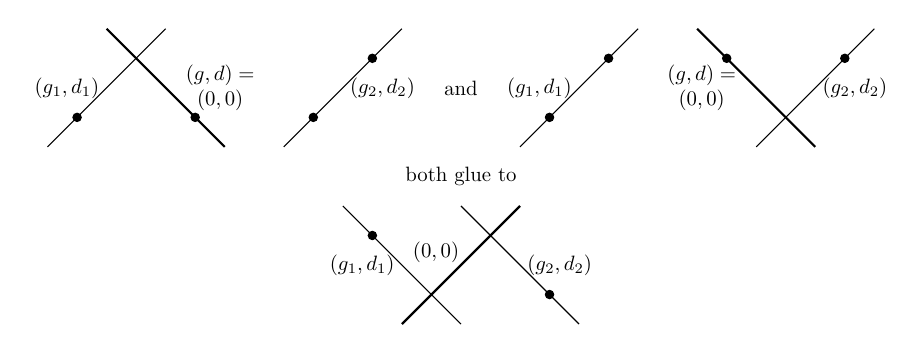
\begin{tikzpicture}[scale=.75,every node/.style={transform shape}]
  \draw (0,0) -- node[left]{$(g_1,d_1)$} (2,2);
  \draw[thick] (1,2) -- node[right]{\begin{tabular}{c} $(g,d)=$ \\ $(0,0)$ \end{tabular}} (3,0);
  \draw[fill=black] (.5,.5) circle[radius=2pt] (2.5,.5) circle[radius=2pt];
  \draw (4,0) -- node[right]{$(g_2,d_2)$}(6,2);
  \draw[fill=black] (4.5,.5) circle[radius=2pt] (5.5,1.5) circle[radius=2pt];
  
  \draw (7,1) node{and};
  
  \draw (8,0) -- node[left]{$(g_1,d_1)$} (10,2);
  \draw[fill=black] (8.5,.5) circle[radius=2pt] (9.5,1.5) circle[radius=2pt];
  \draw[thick] (11,2) -- node[left]{\begin{tabular}{c} $(g,d)=$ \\ $(0,0)$ \end{tabular}} (13,0);
  \draw (12,0) -- node[right]{$(g_2,d_2)$} (14,2);
  \draw[fill=black] (11.5,1.5) circle[radius=2pt] (13.5,1.5) circle[radius=2pt];

  \draw (7,-.5) node{both glue to};
  
  \draw (5,-1) -- node[left]{$(g_1,d_1)$}(7,-3) (7,-1) -- node[right]{$(g_2,d_2)$} (9,-3);
  \draw[thick] (6,-3) -- node[above left=-.1cm]{$(0,0)$} (8,-1);
  \draw[fill=black] (5.5,-1.5) circle[radius=2pt] (8.5,-2.5) circle[radius=2pt];
\end{tikzpicture}
\end{center}
Nevertheless $\psi$ has a natural perfect obstruction theory, given by $\LL_{\psi}$: we only need to show that it is supported in $[-1,0]$. Consider the exact triangle:
\begin{equation*} \psi^* \LL_{\MM_{g,n,\beta}^{\operatorname{wt}}} \to \LL_{\MM_{G,A,B}^{\operatorname{wt}}} \to \LL_\psi \xrightarrow{[1]} \end{equation*}
The first two terms are concentrated in degrees $[0,1]$, because they are the cotangent complexes of smooth Artin stacks. Therefore $\LL_\psi$ is concentrated in degrees $[-1,1]$. Furthermore, if we examine the long exact cohomology sequence near $\h^1(\LL_\psi)$ we find
\begin{equation*} \h^1(\psi^* \LL_{\MM_{g,n,\beta}^{\operatorname{wt}}}) \to \h^1(\LL_{\MM_{G,A,B}^{\operatorname{wt}}}) \to \h^1(\LL_\psi) \to 0 \end{equation*}
and hence we must show that the first map is surjective. But this is dual to the map which takes an infinitesimal automorphism of the disconnected curve to an infinitesimal automorphism of the corresponding connected curve (obtained by glueing together the ``nodal'' marked points). The space of infinitesimal automorphisms of a nodal curve splits into a direct sum of infinitesimal automorphisms of each component; since the glueing does not affect the components, we see that this map is an isomorphism. Hence $\h^1(\LL_\psi) = 0$ as claimed; morally this follows from the fact that the fibres of $\psi$ are Deligne--Mumford.

Hence there is a virtual pull-back map $\psi^!$ which defines a class
\begin{equation*}\psi^! \virt{\Q{g}{n}{X}{\beta}} \end{equation*}
on $\mathcal{D}^{\mathcal{Q}}(X,G,A,B)$. This is the same class as the one induced by the following perfect obstruction theory
\begin{equation*} \varphi^* \EE_{\rho_Q} \to \LL_{\rho_D} \end{equation*}
by functoriality of virtual pull-backs.

Finally if we look at \eqref{Product diagram} we see that $\ev_q^* \LL_{\Delta_{X^r}} \to \LL_h$ is a perfect obstruction theory for the map $h$. To summarise, we have a triangle
\begin{equation}\label{D-E-triangle}
 \begin{tikzcd}
  \D{X}{G,A}{B} \ar[dr,"\rho_D" below=0.1cm] \ar[rr,"h"] & & \E{X}{G,A}{B}\ar[dl,"\rho_E"] \\
& \MM_{G,A,B}^{\operatorname{wt}} &
 \end{tikzcd}
\end{equation}
where all three morphisms are equipped with perfect obstruction theories. We simply need to check that these fit together in a compatible triple.

\begin{lemma} \label{Lemma product class equals pullback class} There is a compatible triple
\begin{equation*}(h^* \EE_{\rho_E}, \varphi^*\EE_{\rho_Q}, \ev_q^*\LL_{\Delta_{X^r}}) \end{equation*}
for the triangle \eqref{D-E-triangle}. Hence by functoriality of virtual pull-backs we have:
\[
 \psi^!\virt{\Q{g}{n}{X}{\beta}}=\Delta_{X^r}^!\virt{\E{X}{G,A}{B}} = \virt{\D{X}{G,A}{B}}
\]
\end{lemma}
\begin{proof}
 We need to construct a morphism of triangles
 \bcd
 h^*\EE_{\rho_E}\ar[r]\ar[d] & \varphi^*\EE_{\rho_Q}\ar[r]\ar[d] & \ev_q^*\LL_{\Delta_{X^r}}\ar[r,"{[1]}"]\ar[d] & {} \\
 h^* \LL_{\rho_E}\ar[r] & \LL_{\rho_D}\ar[r] & \LL_h\ar[r,"{[1]}"] & {}
 \ecd
 
 Consider the following diagram:
\bcd
h^* \tilde{\mathcal{C}} \ar[r,"\nu"] \ar[rd,"\eta" below] & \varphi^* \mathcal{C} \ar[r] \ar[d] \ar[rd,phantom,"\square" right] & \mathcal{C} \ar[d,"\pi"] \\
& \D{X}{G,A}{B} \ar[r,"\varphi"] & \Q{g}{n}{X}{\beta}
\ecd
Here $\tilde{C}$ is the universal (disconnected) curve over $\E{X}{G,A}{B}$, which we have pulled back to $\D{X}{G,A}{B}$, while $\varphi^* \mathcal{C}$ is the universal curve over $\D{X}{G,A}{B}$. Therefore the map $\nu : h^* \tilde{\mathcal{C}} \to \varphi^* \mathcal{C}$ is (fiberwise) a partial normalisation map given by normalising the nodes which connect the ``trunk'' of the centipede to the ``legs.''

There are natural sheaves $\mathcal{F}$ and $\tilde{\mathcal{F}}$ on $\mathcal{C}$ and $h^* \tilde{\mathcal{C}}$ respectively, such that
\begin{align*} \varphi^*\EE_{\rho_Q}^\vee & = \R \pi_* \mathcal{F} \\
h^* \EE_{\rho_E}^\vee & = \R \eta_* \tilde{\mathcal{F}} \end{align*}
Furthermore $\nu^*\mathcal{F}\simeq\tilde{\mathcal{F}}$, hence by tensoring the partial normalisation short exact sequence
\begin{equation*} 0 \to \OO_{\varphi^*{\mathcal{C}}} \to \nu_* \OO_{h^* \tilde{\mathcal{C}}} \to \OO_q \to 0 \end{equation*}
with $\mathcal{F}$ and applying the projection formula, we obtain
\begin{equation*} 0 \to \mathcal{F} \to \nu_* \tilde{\mathcal{F}} \to \mathcal{F}_q \to 0 \end{equation*}
on $\varphi^*\mathcal{C}$, where $q$ is the locus of nodes connecting the trunk to the spine. (The fact that the morphism on the left is injective follows by applying the Snake Lemma to the short exact sequence defining $\mathcal{F}$.) To this we can apply $\R \pi_*$ to obtain an exact triangle
\begin{equation} \label{Normalisation exact triangle} \R \pi_* \mathcal{F} \to \R \eta_* \tilde{\mathcal{F}} \to \R \pi_* \mathcal{F}_q \xrightarrow{[1]} \end{equation}
Finally, notice that, since quasimaps are required not to have base-points at the nodes, the fibre of the sheaf $\mathcal F$ at each of the nodes $q$ can actually be identified with the tangent to the toric variety $X$ at the image of the node itself, i.e. $\R \pi_* \mathcal{F}_q \cong \ev_q^* \TT_{X^r}= \ev_q^* \mathbf{\operatorname{T}}_{\Delta_{X^r}}[-1]$. Dualising sequence \eqref{Normalisation exact triangle} we obtain
\begin{equation*} h^* \EE_{\rho_E} \to \varphi^* \EE_{\rho_Q} \to \ev_q^* \EE_{\Delta_{X^r}} \xrightarrow{[1]} \end{equation*}
as required. \end{proof}
\subsection{Comparison with the GIT construction} \label{Section comparison with GIT construction}

Let $X$ be a smooth projective toric variety and $Y \hookrightarrow X$ a smooth very ample hypersurface. The complete linear system $|\OO_X(Y)|$ gives an embedding $i : X \hookrightarrow \PP^N$ which expresses $Y$ as the intersection inside $\PP^N$ of $X$ and a certain hyperplane $H$: $Y=X\cap H = i^{-1}(H)$. We can \ilemph{define} the moduli space of quasimaps to $Y$ via the following cartesian diagram:
\bcd
\Q{g}{n}{Y}{\beta}\ar[d, hook] \ar[r]\ar[rd,phantom,"\square"] & \Q{g}{n}{H}{d} \ar[d, hook] \\
\Q{g}{n}{X}{\beta}\ar[r, "k"] & \Q{g}{n}{\PP^N}{d}
\ecd
where $d=i_*\beta$. This moduli space is easy to describe: let $s_Y$ denote the section of $\OO_X(Y)$ cutting out $Y$ inside $X$. Recall from \S \ref{Subsection relative stable quasimaps} that for any quasimap
\begin{equation*} ((C,x_1,\ldots,x_n),(L_\rho,u_\rho)_{\rho \in \Sigma_X(1)}, (\varphi_m)_{m \in M_X}) \in \Q{g}{n}{X}{\beta} \end{equation*}
we can construct a section $u_Y$ of a line bundle $L_Y$ on $C$, which plays the role of the pull-back of $s_Y$ to $C$. Then
\begin{equation*} \Q{g}{n}{Y}{\beta} \subseteq \Q{g}{n}{X}{\beta} \end{equation*}
consists of those quasimaps such that $u_Y \equiv 0$.

The cartesian diagram above can also be used to endow $\Q{g}{n}{Y}{\beta}$ with a virtual class via virtual (or diagonal) pull-back along $k$. Thus we can define quasimap invariants for $Y$.

On the other hand, $Y$ has the natural structure of a GIT quotient
\begin{equation*} Y = C(Y) \sslash G \end{equation*}
where $C(Y)\subseteq \mathbb A^{\Sigma_X(1)}$ is the affine cone over $Y$ and $G=\Hom_{\mathbb Z}(\Pic(X),\Gm)\cong\Gm^{r_X}$ acts on $C(Y)$ via the natural inclusion
\begin{equation*} \Gm^{r_X}\hookrightarrow \Gm^{\Sigma_X(1)} \end{equation*}
(here $C(Y)\subseteq \mathbb{A}^{\Sigma_X(1)}$ is preserved by $G$ because it is cut out by a homogeneous equation). In \cite{CFKM} moduli spaces of quasimaps are constructed for GIT quotient targets (satisfying a number of conditions, all of which hold for $Y$). There is thus a moduli space
\begin{equation*} \om{Q}^{\operatorname{GIT}}_{g,n}(Y,\beta) \end{equation*}
which admits a virtual class. Hence we have two moduli spaces of quasimaps to $Y$, each equipped with a virtual class, and we want to check that these definitions agree.

Objects of $\om{Q}^{\operatorname{GIT}}_{g,n}(Y,\beta)$ are diagrams of the form
\bcd
P \ar[d,"G"] \ar[r] & C(Y) \\ 
C & \,
\ecd
where $C$ is a prestable curve, $P$ is a principal $G$-bundle and the map $P \to C(Y)$ is $G$-equivariant. Equivalently, an object consists of a prestable curve $C$, a principal $G$-bundle $P$ and a section $u$ of the associated $C(Y)$-bundle:
\bcd
P\times_{G} C(Y) \ar[d,"p" left] \\
C \ar[u,bend right,"u"right]
\ecd
The obstruction theory on this space is defined relative to the stack $\mathfrak{Bun}_{G}$ parametrising principal $G$-bundles on the universal curve:
\begin{equation*} \mathcal{C}_{\MM_{g,n}} \to \MM_{g,n} \end{equation*}
It is given by
\begin{equation*} \EE_{\om{Q}/\mathfrak{Bun}_G}^\vee = \R \pi_* (u^*\TT_p) \end{equation*}
where $\pi$ is the universal curve over $\om{Q} = \om{Q}^{\operatorname{GIT}}_{g,n}(Y,\beta)$ and $\TT_p$ is the relative tangent complex. There is a natural isomorphism
\begin{equation*} \mathfrak{Bun}_{G}^{g,n} \cong \times^{r_X}_{\MM_{g,n}} \mathfrak{Pic_{g,n}} \end{equation*}
given by sending $P$ to the $r_X$ individual factors of the affine bundle $P\times_{G}\mathbb A^{r_X}$. Furthermore there is a $G$-equivariant embedding
\bcd
P\times_{G} C(Y) \ar[r,hook, "j"]\ar[d,"p" left] & P\times_{G}\mathbb A^{\Sigma_X(1)}\cong \bigoplus_{\rho\in\Sigma_X(1)} L_{\rho}\ar[dl]\\
C \ar[u,bend right,"u"right] &
\ecd
which expresses $P \times_G C(Y)$ as the vanishing locus of $u_Y$ in $\oplus_{\rho \in \Sigma_X(1)} L_\rho$. This shows that the two definitions of the moduli space agree.

Finally we must compare the virtual classes. Using the normal sheaf sequence for the inclusion $j$ (relative to the base $C$) we obtain a short exact sequence on $C$:
\begin{equation*} 0 \to u^* \TT_p \to \bigoplus_{\rho \in \Sigma_X(1)} L_\rho \to u^* \NN_{P \times_G C(Y)/\oplus_{\rho \in \Sigma_X(1)} L_\rho} \to 0 \end{equation*}
Since $P \times_G C(Y)$ is defined by the vanishing of $u_Y$, we see that the final term is isomorphic to the line bundle $L_Y$ discussed above. Thus as elements of the derived category
\begin{equation*} u^* \TT_p = \left[ \bigoplus_{\rho \in \Sigma_X(1)} L_\rho \to L_Y \right] \end{equation*}
Applying $\R \pi_*$ we obtain on the left hand side the obstruction theory for the GIT moduli space relative $\mathfrak{Bun}_G^{g,n}$. On the other hand, the first term on the right hand side is the obstruction theory for $\om{Q}(X)$ relative the product of the Picard stacks (isomorphic to $\mathfrak{Bun}_G^{g,n}$ via the discussion above) whereas the second term is the relative obstruction theory for $\om{Q}(Y)$ inside $\om{Q}(X)$. Thus the virtual classes agree, as claimed.

\section{Intersection-theoretic lemmas}\label{appendix:intersection}

In this appendix we explicitly define the \emph{diagonal pull-back} along a morphism whose target is unobstructed (used in \cite{Ga}) and verify that this agrees with the virtual pull-back of \cite{Manolache-Pull} when both are defined. We also check that it satisfies some expected compatibility properties.

Consider a morphism of DM stacks $f\colon Y\to X$ over a smooth base $\mathfrak M$, such that $X$ is smooth over $\mathfrak M$ and $Y$ carries a virtual class given by a perfect obstruction theory $\EE_{Y/\mathfrak M}$. Then, for every Cartesian diagram
 \bcd
 G\ar[r,"g"]\ar[d,"q"]\ar[rd,phantom,"\Box"] & F\ar[d,"p"] \\
 Y\ar[r,"f"] & X 
 \ecd
and every class $\alpha\in \Achow_*(F)$, we may define
\[
 f^!_{\Delta}(\alpha)=\Delta_X^!([Y]^\text{vir}\times\alpha)\in \Achow_*(G)
\]
which we call the \emph{diagonal pull-back}. We first show that it coincides with the usual virtual pull-back along $f$ in the presence of a compatible perfect obstruction theory for $f$.

\begin{lemma}\label{lem:diagonal_virtual_coincide}
Assume that there exists a relative obstruction theory $\EE_f$ compatible with $\EE_{Y/\mathfrak M}$ and the standard (unobstructed) obstruction theory for $X$, i.e:
 \bcd
 f^* \LL_{X/\mathfrak M} \ar[r] \ar[d,"\operatorname{Id}"] & \EE_{Y/\mathfrak M} \ar[r] \ar[d] & \EE_f \ar[r,"{[1]}"] \ar[d] & \, \\
 f^* \LL_{X/\mathfrak M} \ar[r] & \LL_{Y/\mathfrak M} \ar[r] & \LL_f \ar[r,"{[1]}"] & \,
 \ecd
 Then for every Cartesian diagram and every class $\alpha\in \Achow_*(F)$ as above,
 \[
  f^!_{\operatorname{v}}(\alpha)=f^!_\Delta(\alpha).
 \]
\end{lemma}
\begin{proof}

Consider the following cartesian diagram:
\bcd
G \ar[r,"q \times g"] \ar[d,"g"] \ar[rd,phantom,"\square"] & Y\times_{\mathfrak M}F \ar[r,"\pr_1"] \ar[d,"f \times \Id"] \ar[rd,phantom,"\square"] & Y \ar[d,"f"] \\
F \ar[r,"p \times \Id"] \ar[d,"p"] \ar[rd,phantom,"\square"] & X\times_{\mathfrak M} F \ar[r,"\pr_1"] \ar[d,"\Id \times p"] & X \\
X \ar[r,"\Delta_X"] & X\times_{\mathfrak M}X &
\ecd
Then, by commutativity of (virtual) pull-backs, we have
\begin{align*} \Delta_X^!([Y]^\text{vir}\times\alpha) & = \Delta^!((f^!_{\operatorname{v}}[X])\times\alpha) \\
& = \Delta_X^!(f^!_{\operatorname{v}}([X]\times\alpha)) \\
& = f^!_{\operatorname{v}}(\Delta_X^!([X]\times\alpha)) \\
& = f^!_{\operatorname{v}}(\alpha)
\end{align*}
as required.
\end{proof}

Secondly, we show that the diagonal pull-back behaves similarly to an ordinary virtual pull-back (e.g. commutes with other virtual pull-backs) even in the absence of a compatible perfect obstruction theory.

\begin{lemma} The diagonal pull-back morphism as defined above commutes with ordinary Gysin maps and with virtual pull-backs. \end{lemma}
\begin{proof} First consider the case of ordinary Gysin maps. We must consider a cartesian diagram:
\bcd
Y^{\prime \prime} \ar[r] \ar[d] \ar[rd,phantom,"\square"] & X^{\prime \prime} \ar[r] \ar[d] \ar[rd,phantom,"\square"] & S \ar[d,"k"] \\
Y^\prime \ar[r] \ar[d] \ar[rd,phantom,"\square"] & X^\prime \ar[r] \ar[d] & T \\
Y \ar[r,"f"] & X
\ecd
with $k$ a regular embedding and $f\colon Y\to X$ as before. We need to show that for all $\alpha \in A_*(X^\prime)$:
\begin{equation*} k^! f_{\Delta}^!(\alpha) = f^!_{\Delta} k^!(\alpha) \end{equation*}
We form the cartesian diagram
\bcd
Y^{\prime \prime} \ar[r] \ar[d] \ar[rd,phantom,"\square"] & Y\times X^{\prime \prime} \ar[r] \ar[d] \ar[rd,phantom,"\square"] & S \ar[d,"k"] \\
Y^\prime \ar[r] \ar[d] \ar[rd,phantom,"\square"] & Y\times X^\prime \ar[r] \ar[d] & T \\
X \ar[r,"\Delta_X"] & X\times X &
\ecd
and apply commutativity of usual Gysin morphisms. In the case where $k$ is not a regular embedding but rather is equipped with a relative perfect obstruction theory, the same argument works with $k^!$ replaced by $k_{\text{v}}^!$.
\end{proof}

\bibliographystyle{alpha}
\bibliography{relqm}

\bigskip\bigskip

\noindent Luca Battistella\\
Department of Mathematics, Imperial College London \\
\texttt{l.battistella14@imperial.ac.uk}\\

\noindent Navid Nabijou \\
Department of Mathematics, Imperial College London \\
\texttt{navid.nabijou09@imperial.ac.uk}



\end{document}